%!TEX root = ../thesis.tex
% chktex-file 1
% chktex-file 24
%*******************************************************************************
%****************************** Fifth Chapter **********************************
%*******************************************************************************
% Temperature Resilient Analog/Digital Converter ==> TRAD Converter
\chapter{A new mixed ADC topology}
\label{sec:adc-implementation}

% **************************** Define Graphics Path **************************
\ifpdf 
    \graphicspath{{Chapter4/Figs/Raster/}{Chapter4/Figs/PDF/}{Chapter4/Figs/}}
\else
    \graphicspath{{Chapter4/Figs/Vector/}{Chapter4/Figs/}}
\fi

\section{Architectural Study}
The goal of this research project is to define and to implement a low-OSR ADC for high-speed conversion at 20 MSamples/s with a high-resolution within the smallest silicon area possible. Based on 40 years literature in the ADC domain, only one kind of ADC is not sufficient to match the different desires within 5-clock cycles. A cascade of sub-ADCs seems more promising. Within 5 clock cycles per sample, sub-ADC do not give enough bits as well as the SAR, the algorithmic, the folding, or the counting. And a full-flash converter would exceed the 15 mW budget we fixed for the ADC\@.

Aware of the large resolution drop at high temperature, and with a high-sensitivity to process variations, a true pipelined ADC cannot be used as is considering the area, and the power consumption. Over an extended temperature range from -40\(\degree \)C to +175\(\degree \)C, an ADC having each stage of a different kind would allow us to mix strength and weakness of each one, to reduce the area overhead and the power consumption.

We propose in this section some candidate topologies for the realization of a high performance ADC\@. The main functional characteristics of these stages are gathered at the Table~\ref{tbl:stage-charac}.

\begin{table}[htp]
	\centering
	\caption{Functional characteristics of mainstream architecture presented in Section~\ref{sec:soa}}
	\label{tbl:stage-charac}
	\begin{tabular}{lccccc}
		\toprule
				& Oversampled & \begin{tabular}[c]{@{}l@{}}Precision/stage\\ 1-bit converter\end{tabular} & \begin{tabular}[c]{@{}l@{}}Sample \& Hold\\ required\end{tabular} & \begin{tabular}[c]{@{}l@{}}Has a\\ residue\end{tabular} & \begin{tabular}[c]{@{}l@{}}multibit convertion\\ possible\end{tabular} \\ \midrule
					Pipelined   & No          & 1                                                                         & NA                                                                & Yes           & Yes                                                                      \\
					Counting    & Yes         & $log_2(OSR)$                                                               & Yes                                                               & Yes           & Yes                                                                      \\
					Algorithmic & Yes         & $OSR$                                                                       & No                                                                & Yes           & Yes                                                                      \\
					Flash       & No          & 1                                                                         & NA                                                                & No            & Yes                                                                      \\
					SAR         & Yes         & $OSR-1$                                                                     & No                                                                & No\footnotemark           & No \\  \bottomrule                                                                     
	\end{tabular}
	\end{table}

\footnotetext{at the price of extra area and power consumption to sample and hold or to buffer}

All kinds of stages cannot be connected together due to topological constraints. To list some of them, Flash and SAR stages should always be the last stage as they produce no residue. If the SAR is not the last-stage, an extra amplification with high gain is required at the output of the SAR\@. When counting stages are cascaded, a sample and hold stage is required between them. And considering the sensitivity to non-idealities and noise filtering, counting stages should be used before algorithmic ones.

As a rule of thumb, to reduce the area, the topology of the ADC should minimize the total amount of components. In consequence, the resources required for each kind of stage are gathered at the next table where N is the number of digital levels produced by the stage.

\begin{table}[htp]
	\centering
	\caption{Mandatory resources to estimate the area required and the potential intrinsic noise contributor}
	\label{tbl:stages-ressources}
	\begin{tabular}{@{}lcccc@{}}
	\toprule
	(For Single-Ended implementation)  & Comparators & OTA & Capacitors& Switches       \\ \midrule
	Pipelined                                                      & $N-1$         & 1   & 2                                                                   & $5+N$            \\
\begin{tabular}[c]{@{}l@{}}First Order\\ Counting\end{tabular} & $N-1$         & 1   & 2                                                                   & $4+N$            \\
	Algorithmic                                                    & $N-1$         & 1   & 2 / 3                                                               & $5+N$ / $4+2(N-1)$ \\
	Flash                                                          & $N-1$         & 0   & 0                                                                   & 0              \\
	SAR                                                            & 1           & 0   & $2^{OSR-1}$                                        & $3(OSR-1)$       \\ \bottomrule
	\end{tabular}
\end{table}

From all these constraints, we deduce some possible candidates to achieve the resolution of 12-bits with a limited oversampling ratio.
A MASH or an Extended-Range followed by a last sub-ADC of any kind benefit from the noise shaping of the $\Delta\Sigma$ modulation with a limited sensitivity to analog defects with few components.

\subsection{Pipelined of Counting ADCs}
The converter is composed with several counting stages, each of them being composed with first-order or second-order sigma delta. The clock frequency of the
counting stages is the Nyquist frequency multiplied by the OSR of the converter. In the case of first order counters, The resolution is the ADC resolution multiplied by \(log_2(OSR)\). For example, with a 3-level ADC and OSR=5, the resolution of each counting stage is approximately 3.5 bits.

Among the three configurations of the \figurename~\ref{fig:counting-candidates}, the first one is made of 4 first order Incremental-\(\Delta \Sigma\) modulator. The maximum reachable resolution is therefore a 14 bits one. At a clock frequency of 100 MHz, the power hungry element is arguably the OTA\@. Built around 4 of these this configuration is not the most efficient one and the total area becomes large.

The last stage could also be a Flash or a SAR\@. Only using 3 OTAs, the power consumption is more reasonable. The second configuration, with a flash at the end, is able to achieve a 13.5-bits resolution with the employ of 13 comparators. The power and area of 1 OTA are now allocated to 5 extra comparators. Willing a fully differential implementation of the design, the choice in favor of this configuration is not justified.

As soon as the OSR is high-enough, the SAR technology will be more efficient that the FLASH in terms of area and consumption. And this last configuration is the most promising out of those three. The power budget of 15 mW at 20 Msamples/s sounds reachable based on an architecture quite similar: in~\cite{Liu2017} a 1-1-1 MASH CT-\(\Delta\Sigma\) consumes 19.7 mW at 50 Msamples/s in a 40 nm technology supplied at only 1.2 V for a resolution of 11-bits.

\begin{figure}[htp]
	\centering
	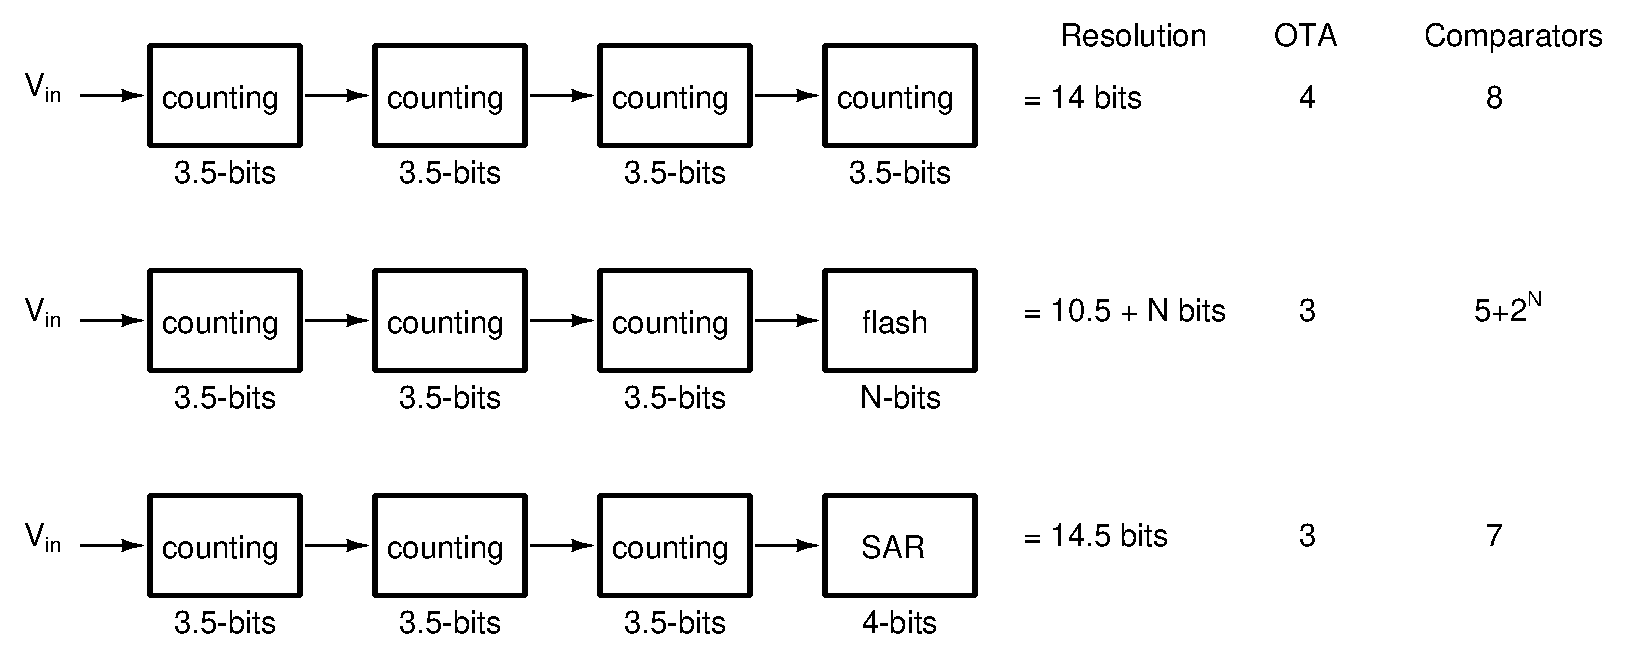
\includegraphics[width=.9\textwidth]{Chapter4/Figs/study/counting-conversion.ps}
	\caption{Possible candidates leveraging the strength of the \(\Delta \Sigma\) modulation to achieve the expected resolution with the resources needed}
	\label{fig:counting-candidates}
\end{figure}

\subsection{Extended-Range with extra stage}
The topologies in this section are composed with two kinds of stages: counting and algorithmic. A final stage of a third kind such as a SAR is proposed. Algorithmic stages are the most sensitive to non-idealities. This is why they always follow and not precede the counting stages.

The forth configuration of these last three is similar to previous ones. The 1-1 MASH at the input is the least sensitive to non-idealities while the noise shaping is still effective at low-OSR\@. Despite this, the algorithmic copes clumsily with transistor non-linearity. And a 2-bit flash is sufficient to make a 13.5-bit ADC with in total 9 comparators. Therefore, this solution is expected a larger silicon footprint than the third possible configuration.

\begin{figure}[htp]
	\centering
	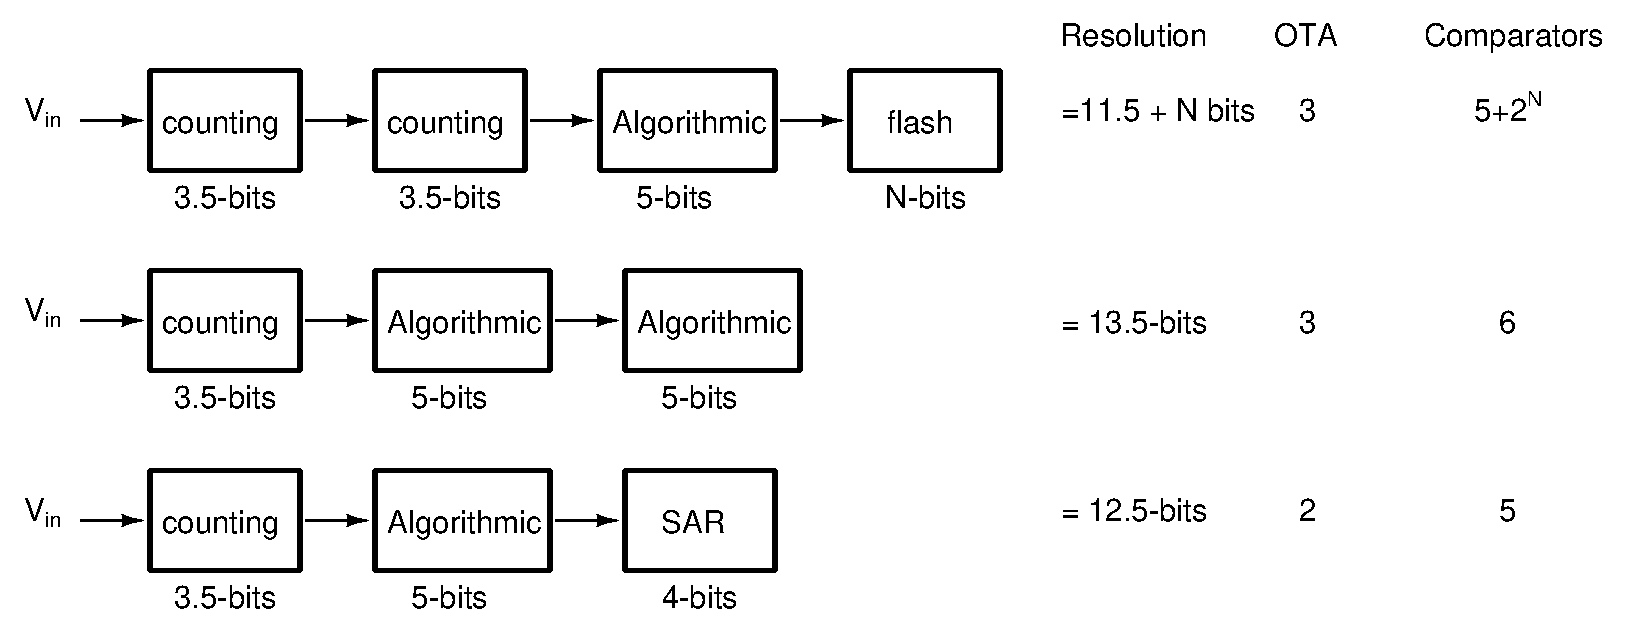
\includegraphics[width=.9\textwidth]{Chapter4/Figs/study/counting-algo-conversion.ps}
	\caption{Possible candidates leveraging the strength of the \(\Delta \Sigma\) modulation and the fast signal information extraction of the algorithmic with the resources required }
	\label{fig:counting-algo-candidates}
\end{figure}

The fifth proposal gets rid of a stage and 3 comparators to achieve the same resolution. Unfortunately, the analog defects have a deeper impact due to the presence of two consecutive algorithmic stages. The last proposal replaces the final stage for a SAR having only one comparator. The advantages are three fold: first, the SAR scales well with the technology while it consumes very few. Second, the number of OTA is reduced to only two for the sake of power consumption saving. And third, this architecture is less sensitive to analog non-linearity.

Among the six different configurations which have been proposed, the last configuration uses three different architectures to reduce the footprint, the power consumption while preserving a reachable resolution greater than 12-bits. In consequence, the latter is selected for the design of the new harsh environment ADC\@.

\subsection{The selected topology}
\label{sec:selected-topology}
Previous sections briefly presents the possible candidates and the reasons of the proposed architecture. The current design of the proposal is based for an oversampling ratio of 5, but allows us to perform conversions with an oversampling ratio of 6. In consequence, the SAR is designed in this way while the two first stage design is OSR independent. The selected architecture is represented in \figurename~\ref{fig:early-prop-adc-architecture} with more details about the operation and resources involved. While a severe drop of 2 bits can be experienced over 150\(\degree \)C as in~\cite{Ericson2004}, Reaching a maximum of 12.5-bits is not sufficient.

\begin{figure}[htp]
	\centering
	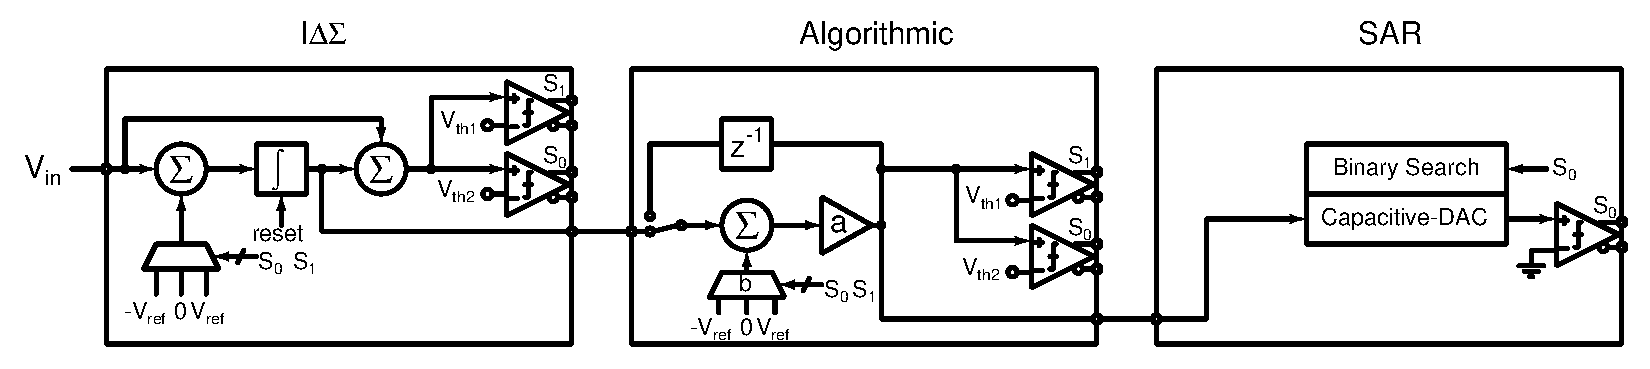
\includegraphics[width=\textwidth]{Chapter4/Figs/architecture-full-principle.ps}
	\caption{Early proposition of the ADC architecture}
	\label{fig:early-prop-adc-architecture}
\end{figure}

To provide extra margin, the modification highlighted in \figurename~\ref{fig:final-prop-adc-architecture} consists in adding an extra comparator \(S_2\) of the second stage to extract the polarity of the second stage residue. The comparison results corresponds to the first decision made by a binary search algorithm such as the one used in the last stage. By an appropriate threshold voltage for comparators of the 3-levels quantizer previously used (\(S_0, S_1 \)), leads to the third stage second decision.

\begin{figure}[htp]
	\centering
	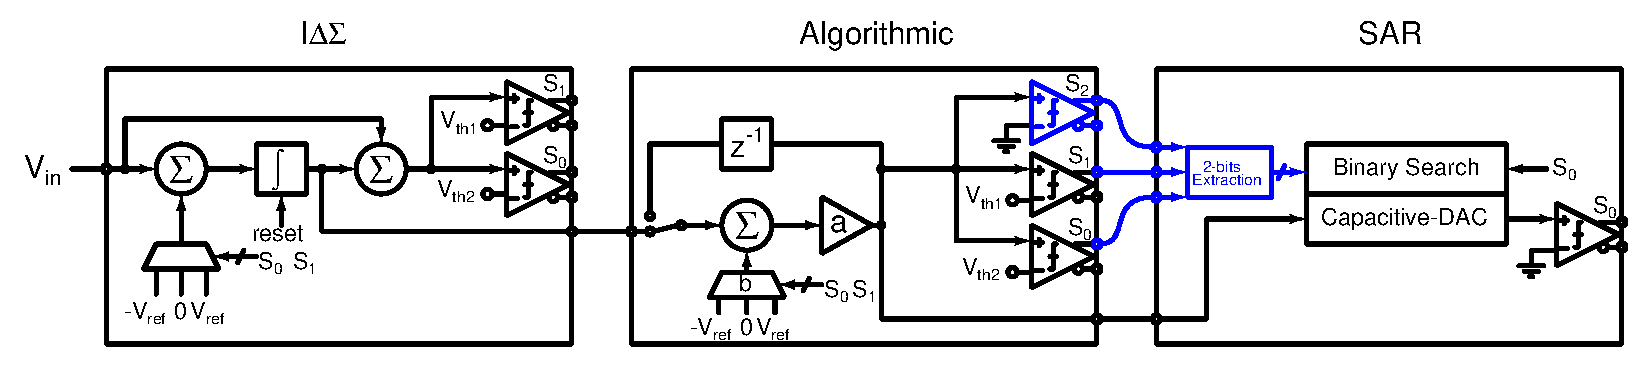
\includegraphics[width=\textwidth]{Chapter4/Figs/architecture-full-principle-final.ps}
	\caption{Final proposition of the ADC architecture}
	\label{fig:final-prop-adc-architecture}
\end{figure}

The change of the bits distribution into 4-bits from the second stage, and 6-bits for the last stage allows us to extract 1 extra bit. The next section discusses in detail the implementation of the selected architecture depicted in \figurename~\ref{fig:final-prop-adc-architecture}.

\section{Sub-ADC Analysis}
\subsection{Incremental-\(\Delta\Sigma \)} % section 5.1

\textbf{\textcolor{black}{principle and the basic choice:}}
The first stage is a fully-differential Incremental-\(\Delta\Sigma \) modulator based on the principle given in section~\ref{sec:soa-isd}.
Compared to a conventional $\Delta\Sigma$ modulator, the integrator is reset at each new sample to mimic a nyquist rate ADC\@. Therefore, the design of an \(I\Delta\Sigma \) requires OSR+1 clock cycles to achieve an oversampling ratio of OSR\@. The version presented in the State of the Art was a multi-bit quantizer to be generic. However, the 1-bit quantizer is the simplest and is inherently linear. In consequence, a first-order Incremental-$\Delta\Sigma$ with 1-bit quantizer is the most robust solution.

\textbf{\textcolor{black}{limitations:}}
Kept as a basis for the first stage of our ADC, the 1-bit quantizer in this topology does not limit the excursion of the integrator output. Without this limitation of the output swing, a large constraint is placed on the amplifier inside the integrator, and results in an integrator output deformed and outside of the allowed input swing of the following stage. In order to suppress this eventuality, two key actions have been implemented.

\textbf{\textcolor{black}{solutions:}}
First, the two comparators instead of one detects when the output of integrator, also called the residue, is outside the desired excursion range. Second, the input voltage is summed with the integrator output before the comparison to the excursion range limits. The input has a feed-forward path not to saturate the integrator by summing the residue with the input signal.

\textbf{\textcolor{black}{solution 1 (3-levels quantizer):}}
Let us assume the output of comparators is either zero or one, and we call the quantification error $e(z)$, the error between the input voltage of the quantizer $x(z)$, and the estimation coming from the comparators' outputs. The estimation performed by the 3-levels quantizer is thus \((S_1(z)+S_0(z)-1)V_{\rm ref} \), if we consider $S_1(z)$ and $S_0(z)$ the comparators' outputs in the z-domain. The value of the estimation is one among those in the following set \(\{-1,0,1\}\). The quantification error is thus given to be
\begin{equation} 
	e(z) = x(z) - (S_1(z)+S_0(z)-1)V_{\rm ref}
\end{equation}

To estimate the repercussion on the output of the integrator called Residue, we describe the modulator using the z-transform in the equation~(\ref{eqn:modulator-z-transform}).
\begin{eqnarray}
	\label{eqn:modulator-z-transform}
\frac{V_{\rm in}(z)z^{-1}-(S_1(z)+S_0(z)-1)V_{\rm ref}z^{-1}}{1-z^{-1}} + V_{\rm in}(z) + e(z) = (S_1(z)+S_0(z)-1)V_{\rm ref}  \\
e(z) = \frac{(V_{\rm ref}(S_1(z)+S_0(z)-1)-V_{\rm in}(z))}{1-z^{-1}}
\end{eqnarray}
Based on the latter, the output of the integrator is thus defined by 
\begin{equation}
	{\rm Residue}(z) = -\frac{e(z)z^{-1}}{1+z^{-1}}
\end{equation}
To minimize the Residue, \(e(z) \) shall be minimized too. 

\textbf{\textcolor{black}{error minimization:}}
From the definition of quantification error, at the $n^{\text{th}}$-clock cycle, \(e[n]\) can be expressed as a function of the threshold voltages and the input swing of the quantizer delimited in the range $[x_{\min}, x_{\max}]$. This is given in equation~(\ref{eqn:quantizer-error-function}).
\begin{equation}
	\label{eqn:quantizer-error-function}
	e[n](x) = 
\begin{cases}
	\frac{2}{x_{\max}-x_{\min}}(x-x_{\max}),& \text{if } x > V_{\rm th2} \\
	\frac{2}{x_{\max}-x_{\min}}x  ,& \text{if } x \in [V_{\rm th1}, V_{\rm th2}] \\
	\frac{2}{x_{\max}-x_{\min}}(x-x_{\min}),& \text{otherwise}
\end{cases}
\end{equation}

Graphically, the error function is depicted in \figurename~\ref{fig:3-levels-error-pattern} with the extrema values.
\begin{figure}[htp]
	\centering
	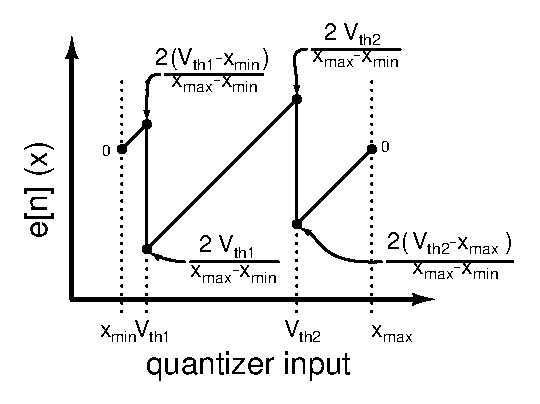
\includegraphics[width=0.5\textwidth]{Chapter4/Figs/3-levels-pattern.ps}
	\caption{3-levels error pattern}
	\label{fig:3-levels-error-pattern}
\end{figure}

\textbf{\textcolor{black}{error minimization (threshold voltages tuning):}}
As the structure is fully differential a constraint of symmetry on the threshold voltage is equivalent to impose the same output swing for both the positive and negative signal of the integrator around the common-mode voltage. This assumption being reasonable, the error \(e[n](x) \) is minimal when \(V_{\rm th2}=-V_{\rm th1}=\frac{x_{\max}-x_{\min}}{2} \).

\textbf{\textcolor{black}{solution 2 (input feed-forward):}}
The second solution to control the excursion of the integrator output consists in the addition of a feed-forward input path. For the sake of clarity the modulator is represented as a single-ended topology in \figurename~\ref{fig:isd-alone-clk-cycle}. This figure represents the normal behaviour of the modulator. Being incremental, the integrator is reset at the beginning of each new sample: during the first clock cycle. Without the feed-forward path, the decision of the 3-levels quantizer in this clock cycle is irrelevant. And the integrator will increment by the value of the input at the second clock cycle. With this input path, the input voltage is estimated from the first clock cycle. And a feedback is applied then. The integrator does not have the possibility to exceed the limit fixed as the increment is the error between the input and its pre-estimation.

Besides that, the input feed-forward is beneficial for the modulator in the configuration depicted in \figurename~\ref{fig:isd-alone-std-clk-cycle}. Without the input feed-forward, the integrator has to process the quantization noise in addition to the input signal for the regulation of the output. On the other hand, the integrator has to process only the quantization noise. And the removal of the input signal component reduces the swing at the internal nodes of the modulator which relaxes the headroom requirements, and allows for more efficient amplifier architectures to be used. However, the input-feed-forward path presents complications, a timing constraint overhead and the analog adder at the quantizer input.

This given, the adder can be implemented as an active analog bloc or as a passive one. For power saving reason, a bunch of capacitors forms the passive adder.

\begin{figure}[htp]
	\centering
	\begin{subfigure}[b]{0.48\textwidth}
		\centering
		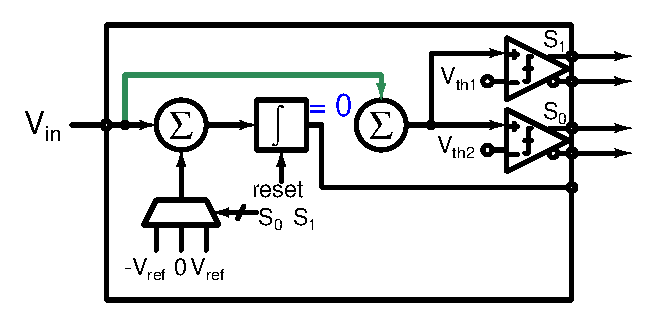
\includegraphics[width=\textwidth]{Chapter4/Figs/isd-principle-reset.ps}
		\subcaption{first clock cycle}
		\label{fig:isd-alone-reset-clk-cycle}
	\end{subfigure}
	\begin{subfigure}[b]{0.48\textwidth}
		\centering
		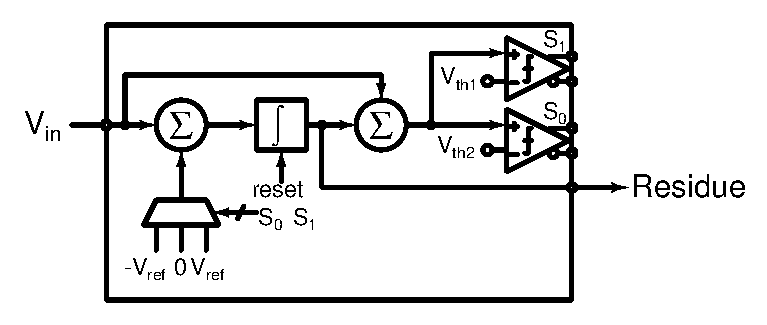
\includegraphics[width=\textwidth]{Chapter4/Figs/isd-principle.ps}
		\subcaption{following clock cycle}
		\label{fig:isd-alone-std-clk-cycle}
	\end{subfigure}
	\caption{3-level \(\Delta\Sigma \) modulator architecture in the ADC and the initialization of a new sample while delivering the
	residue to the next stage}
	\label{fig:isd-alone-clk-cycle}
\end{figure}

\textbf{\textcolor{black}{resolution and strategy:}}
Due to the minimization of the quantification error by selecting the threshold voltages of the quantizer, the residue is bounded to $\pm V_{\rm ref}/2$. The resolution of the ADC can be enhanced by an inter-stage gain of two between this stage, and the one following. This transfer analog constraint on the offset to the second stage with a possible input overflow. With an ability to withstand greater offsets, errors from non-perfectly set threshold voltages, and prevents extra noise source decreasing the SNR of internal nodes, no inter-stage gain is introduced within this stage. With 8-steps in the transfer function of this stage, the maximum resolution is 3-bits.

	\subsubsection{Integrator}              % section 5.1.2
% discuss delta charge redistribution or standard sc integrator
\textbf{\textcolor{black}{principle:}}
The switched capacitor integrator is continuous-time integrator whose resistor is emulated by a switching capacitor. Here in the \figurename~\ref{fig:sigma-delta-integration}, $C_S$ first samples the input voltage during $\Phi_1$ and then delivers its charge to $C_I$ through the virtual ground of the amplifier during $\Phi_2$. Not being reset, at each clock cycle, $C_I$ integrate charges sampled. At the output, the voltage change after each clock period is equal to $-(C_S/C_I)(V_{\rm in} - V_{\rm FB})$.

\begin{figure}[htp]
	\centering
	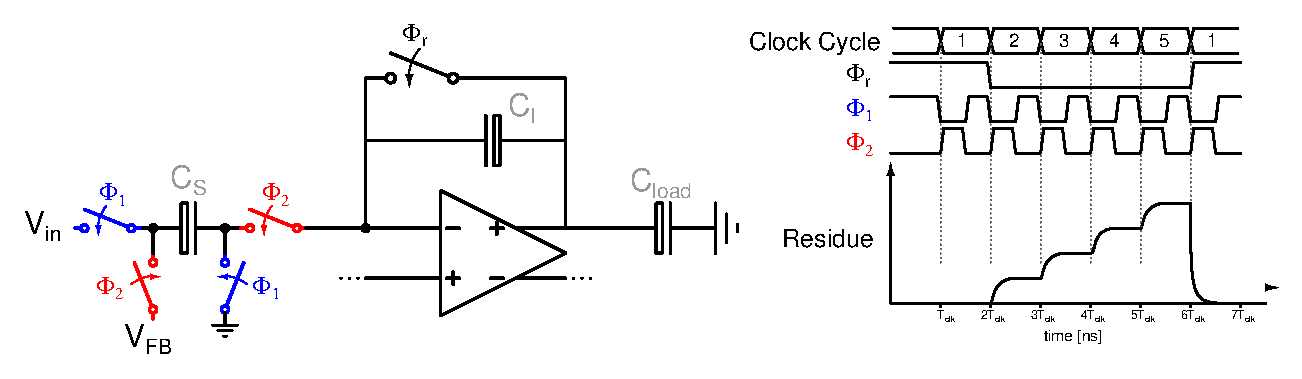
\includegraphics[width=\textwidth]{Chapter4/Figs/sigma-delta-integration.ps}
	\begin{subfigure}[b]{0.48\textwidth}
		\centering
		\subcaption{schematic}
	\end{subfigure}
	\begin{subfigure}[b]{0.48\textwidth}
		\centering
		\subcaption{transient signal}
	\end{subfigure}
	\caption{Principle of switched capacitor integrator}
	\label{fig:sigma-delta-integration}
\end{figure}

\textbf{\textcolor{black}{parasitic insensitive:}}
Suppose $C_S$ has a parasitic capacitance from each plate to ground. While the left plate charge to $V_{\rm in}$ then $V_{\rm FB}$, the parasitic capacitor of this plate has no contribution in the charge transfer during $\Phi_2$. Unfortunately, the right plate parasitic will be charged a little due to the finite gain of the amplifier and appears in the charge transfer as a small voltage drop. This point also applies to the nonlinearities arising from these parasitics.

In addition to this, the implementation using parasitic insensitive switched capacitor integrator requires the use of non-overlapping phases. This is necessary for avoiding the simultaneous activation of switches connecting to the $V_{\rm cm}$ or $V_{\rm refp}$/$V_{\rm refm}$, which would corrupt the value stored on $C_S$, and switches connecting the input voltage and the virtual ground, which would allow Vin to momentarily charge $C_I$ through $C_S$, reducing the integrator gain. 

\textbf{\textcolor{black}{integrator existing modes:}}
In a conventional mode a clock cycle is lost for the reset of the integrator. In the case of a reset done at the first clock cycle of a new conversion, the output bits of the last clock cycle are not related to the residue transfer at this clock cycle. With two bits at each clock cycle, only 8-bits are necessary out of the ten provided. With a low-OSR conversion, each clock cycle is important. One can enhance by adding a switch in the charge transfer path as depicted in \figurename~\ref{fig:sigma-delta-modes-integration}. This switch opens the signal path to shunt the amplifier at each clock cycle without resetting the charge stored in $C_I$. As a result, the residue is falling down to zero at each clock cycle. The amplifier has thus an increased speed and slew-rate constraint. For the implementation, \(\Phi_{1mode} \) is a signal always on to operate in a conventional mode.

\begin{figure}[htp]
	\centering
	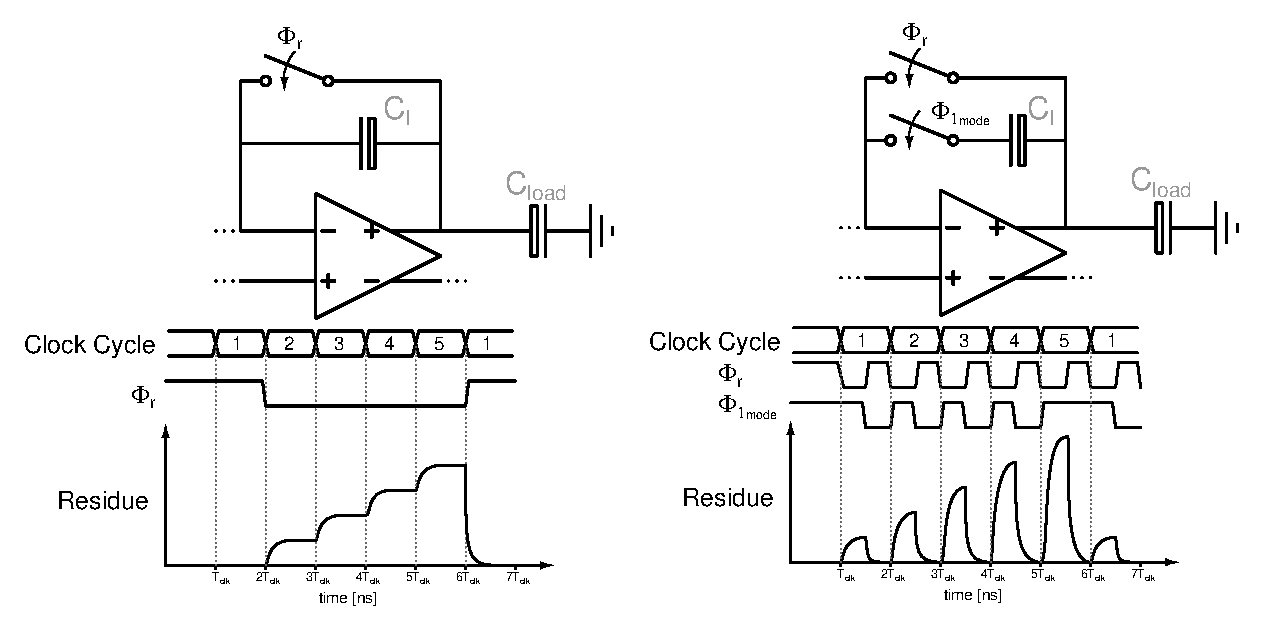
\includegraphics[width=\textwidth]{Chapter4/Figs/sigma-delta-modes-integration.ps}
	\begin{subfigure}[b]{0.48\textwidth}
		\centering
		\subcaption{conventional mode}
	\end{subfigure}
	\begin{subfigure}[b]{0.48\textwidth}
		\centering
		\subcaption{enhanced mode}
	\end{subfigure}
	\caption{Integration without clock cycle loss to enhance performance by amplifier shunt}
	\label{fig:sigma-delta-modes-integration}
\end{figure}

The final representation of the integrator is represented by the \figurename~\ref{fig:isd-sc-integrator} where \(\Phi_1 \) and \(\Phi_2 \) are non-overlapping phase while \(\Phi_{1d} \) and \(\Phi_{2d} \) are respectively their delayed version. \(\Phi_{2d} \) does not overlap with \(\Phi_1 \) too.

\begin{figure}[htp]
	\centering
	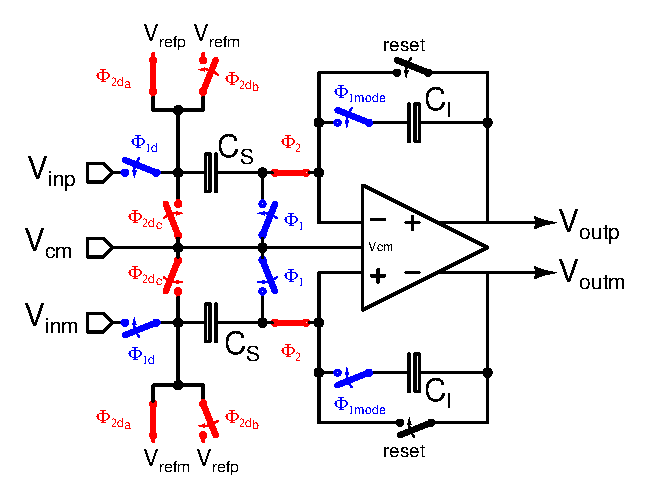
\includegraphics[width=0.6\textwidth]{Chapter4/Figs/sc-integrator-isd.ps}
	\caption{Switched-capacitor integrator implementation}
	\label{fig:isd-sc-integrator}
\end{figure}

\textbf{\textcolor{black}{Reduction of the INL without calibration by the ratio $\mathbf{C_S/C_I}$:}}
In such circumstances the SC-Integrator respects the equation~(\ref{eqn:sc-integrator}) where A is the OTA DC Gain, \(C_S \) the sampling capacitor, \(C_I \) the integration capacitor, and \(V_{\rm in} \), \(V_{\rm ref} \), \(V_{\rm out} \) respectively the differential voltage \(V_{\rm inp}-V_{\rm inm} \), \(V_{\rm refp}-V_{\rm refm} \), and \(V_{\rm outp}-V_{\rm outm} \).
\begin{equation}
    \label{eqn:sc-integrator}
    V_{\rm out}[n] = V_{\rm out}[n-1] \left(\frac{1+\frac{1}{A}}{1+\frac{1+C_S/C_I}{A}}\right) + (V_{\rm in}-b[n-1]V_{\rm ref})\frac{C_S}{C_I}\left(\frac{1}{1+\frac{1+C_S/C_I}{A}}\right)
\end{equation}

As demonstrated in Appendix~\ref{app:integrator-inl}, the INL is tightly linked with the settling error of the integrator after n-steps. Even if this highly depends on the OTA DC Gain, the ratio \(C_S/C_I \) deeply impact it. The settling error is smaller for small \(C_S/C_I \) and the output swing of the integrator is limited by the threshold voltages of the 3-levels quantizer. Unfortunately, for \(C_S/C_I < 1\) ratio and constant noise power from the OTA, it gives more weight to the intrinsic noise of the OTA as each integration step is small. Accordingly a ratio of 1 is preferred leading to a feedback factor \(\beta = C_I/(C_S+C_I) = 1/2 \) for the design of the OTA\@.

%In order to fully use each of them, another integrating capacitor could be added. This capacitor noted \(C_{I2} \) is only used while the first integrator's capacitor \(C_{I1} \) is reset. The extra capacitor in the integrator to deliver the residue processed to the next stage. Meanwhile, the 1.5-bit quantizer is still providing firsts bits of new samples. Despite this solution prevents a clock cycle loss, the mismatch between integration capacitor affects the weight inside the digital counter and a digital calibration is required. Moreover, non-idealities of the OTA introduce a memory effect between each sample due to extra parasitics of switches worsen with the temperature. Therefore, we allow the possibility of a clock cycle loss. The resolution of this stage is thus enhanced by the introduction of an inter-stage gain of 2 between this stage and the following.

\textbf{\textcolor{black}{switches noise:}}
Considering error sources, switches on the signal path is of much importance as they source the signal and induce noise by their finite channel resistance. 
Therefore, the voltage standard deviation of the thermal noise injected by a switch on a capacitance is given to be \(\sqrt{k_BT/C} \) where \(k_B\) is the Boltzmann constant, T the temperature, and C the load capacitance of a switch. On the sampling capacitor, the number of switches connected is $N_{\rm switches} = 6$. To bound the noise variation within an LSB of a given resolution, the following criterion shall be respected: $\sqrt{N_{\rm switches} k_BT/C} < \frac{V_{\rm in_{\max}}-V_{\rm in_{\min}}}{2^{\rm resolution}}$. So, the minimum capacitance to for a desired resolution is $C_{\min} > N_{\rm switches} k_BT \left(\frac{2^{\rm resolution}}{V_{\rm in_{\max}}-V_{\rm in_{\min}}} \right)^2$. As the $\Delta\Sigma$ is oversampling at least over 5 clock cycles, the noise power is divided by OSR\@. For a maximum temperature of 175\(\degree \)C, the sampling capacitor should at least be to 110 fF in order to bound the thermal noise within a 11.7-bits LSB\@.

\textbf{\textcolor{black}{channel resistance and settling time:}}
The second source of error concerning them is the settling error. This error comes from a first order system settling error whose time constant is defined by the product of the finite channel resistance and the sampling capacitance as \(\tau = R_{\rm switches}C_S \). In this regard, two switches in series samples the input voltage with a settling time of 9 ns and an accuracy of 14-bits. The maximum switch resistance follows as 
\begin{equation}
2 R_{\rm switches} = -\frac{T_{\max}}{C_S \times \ln(V_{\rm error})} = - \frac{9 ns}{110 fF \times \ln (1/2^{14})} \approx 8400 \Omega
\end{equation}
This does not consider the voltage dependence of \(\tau \) coming from the non-linear junction capacitance of switches parasitics and the bulk effect of transistors as depicted by the \figurename~\ref{fig:cmos-ron-vin-temp}. In either case, the designed switches on resistance is far below the limit to not be the bottleneck in the settling speed.
\begin{figure}[htp]
	\centering
	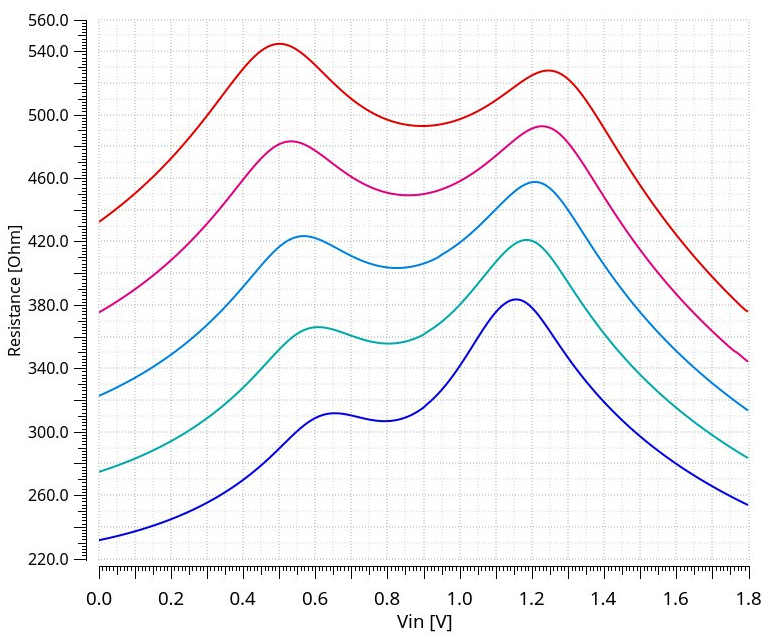
\includegraphics[width=0.5\textwidth]{Chapter4/Figs/xt018_2u_180nm_3-5_resistance.jpg}
	\caption{CMOS switches for a ratio PMOS/NMOS of 3.5 from -40$\degree$C to 175$\degree$C as a function of the input voltage}
	\label{fig:cmos-ron-vin-temp}
\end{figure}

\textbf{\textcolor{black}{charge injection:}}
By the way, charge injection in analog switches and multiplexers is a level change caused by stray capacitance associated with the NMOS and PMOS transistors that make up the analog switch. In a fully differential architecture this phenomenon is fairly reduced, but not annihilated. Indeed, the voltage commuted in the positive side is the opposite of the one in the negative side: at least a voltage dependant error is introduced. In the case of switches connecting the input voltages, the error on the transfer function of the ADC is dependant of the input voltage.

As signal switches shall be complementary ones with at least PMOS 3.5 times larger than NMOS to prevent non-linearity dependant on the input voltage. The charge injected by PMOS stray capacitance are thus not fully absorbed by the NMOS stray capacitance as depicted by \figurename~\ref{fig:charge-injection-switches}. As we assume that the input voltage of the switch is approximately equal to the one sampled on the capacitor \(C_S\), the charge deposited by the NMOS transistor is \(\Delta q = W_nL_nC_{\rm ox}(V_{\rm DD}-V_{\rm in}-V_{\rm thn}) \) while the charge from the PMOS transistor is \(\Delta q = W_pL_pC_{ox}(V_{\rm in}-V_{\rm thp}) \). Hence, size of switches shall be minimal to reduce the charge injection while the increased channel resistance induce distortions.

Finally, the bottom switch connecting the bottom plate of the capacitor to the common mode voltage should turns on/off before the signal switches connect to top plate capacitance. Indeed, in the case of a bottom sampling, switches on the bottom plate inject charge while opening. Injected charge is constant since its gate-source voltage is constant and eliminated when used differentially. Then the bottom plate of \(C_S\) is already floating when its top-plate switch is opened, no signal dependant charge is injected on \(C_S\).

\begin{figure}[htp]
	\centering
	\begin{subfigure}[b]{0.52\textwidth}
		\centering
		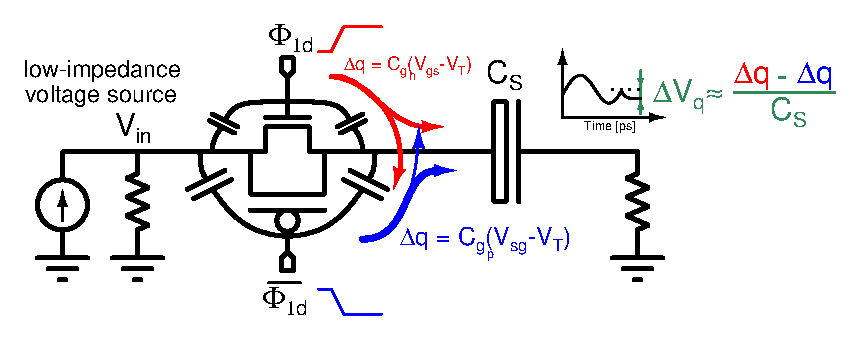
\includegraphics[width=\textwidth]{Chapter4/Figs/charge-injection.ps}
		\subcaption{charge injection}
		\label{fig:charge-injection-switches}
	\end{subfigure}
	\begin{subfigure}[b]{0.46\textwidth}
		\centering
		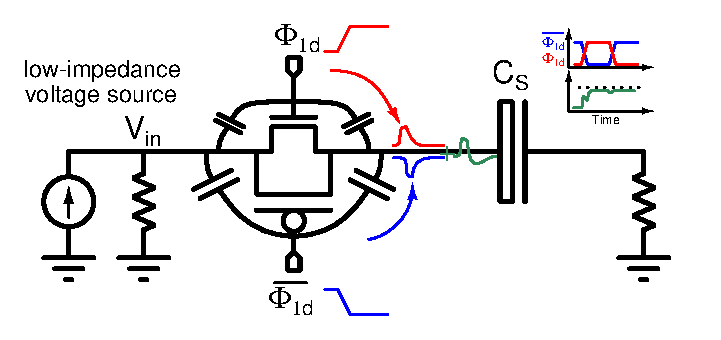
\includegraphics[width=\textwidth]{Chapter4/Figs/clock-feedthrough.ps}
		\subcaption{clock-feedthrough}
		\label{fig:clock-feedthrough-switches}
	\end{subfigure}
	\caption{Phenomenon of charge injection and clock-feed-through on the sampling switches}
	\label{fig:sample-switches-error-source}
\end{figure}

\textbf{\textcolor{black}{clock feedthough:}}
In addition to the charge injection coming from these signal switches, the clock feed-through is an error that is constant with the input voltage level \(\Delta V = V_{\rm gate} \frac{W C_{\rm ov}}{W C_{\rm ov}+C_S}\). For high-speed input signals, it is critical that the NMOS and PMOS switches in \figurename~\ref{fig:clock-feedthrough-switches} turn off simultaneously. If, for example, the NMOS device turns off \(\Delta t\) seconds earlier than the PMOS device, then the output voltage tends to track the input for the remaining \(\Delta t\) seconds, but with a large, input-dependent time constant. This effect gives rise to distortion in the sampled value.

To reduce the amount of charges, the switches size is determined by \(L=L_{\min}\) to minimize the area, and an optimization of their width to reduce the input voltage dependency of this sub-ADC residue in the range from 1\(\mu \)m to 4\(\mu \)m. A good balance is found for \(W/L = \) 2 \(\mu \)m/180 nm with a ratio PMOS over NMOS of 3.5.

% simulation of switches non linearity due to charge injection and then with switches non linearity between NMOS/PMOS.

	\subsubsection{1.5-bit Quantizer}             % section 5.1.3
	\label{sec:isd-3-levels-quantizer}
This given, The passive adder circuit is represented in \figurename~\ref{fig:sc-pacth}. The first clock phase is used to reset the passive adder while the subtractor-integrator is sampling. The second clock phase activates the summation by charging capacitors.

\begin{figure}[htp]
	\centering
	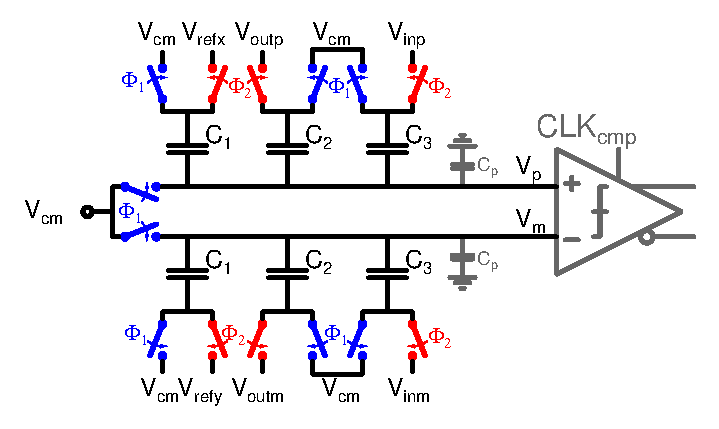
\includegraphics[width=0.75\textwidth]{Chapter4/Figs/isd-passive-adder-comp.ps}
	\caption{Switched capacitor passive adder and comparison to a threshold voltage}
	\label{fig:sc-pacth}
\end{figure}

The choice of appropriate capacitor ratio results from following equations of the differential voltage seen at the input of comparators.

\begin{align}
	V_p &= \frac{C_1V_{\rm refx}+C_2V_{\rm outp}+C_3V_{\rm inp}+0\times C_p}{C_1+C_2+C_3+C_p} \\
	V_m &= \frac{C_1V_{\rm refy}+C_2V_{\rm outm}+C_3V_{\rm inm}+0\times C_p}{C_1+C_2+C_3+C_p}
\end{align}

The differential voltage seen by the comparator is proportional to the first differential input plus a weighted second differential voltage. We can notice that when comparing the input voltage to a weighted reference voltage, the gain is not a concern since only the sign of the differential voltage is important. And determining the sign is equivalent to get the result of the following inequalities (\ref{eqn:passive-adder-ineq}).

\begin{align}
	\label{eqn:passive-adder-ineq}
	V_p > V_m &\equiv C_1V_{\rm refx}+C_2V_{\rm outp}+C_3V_{\rm inp}+0\times C_p > C_1V_{\rm refy}+C_2V_{\rm outm}+C_3V_{\rm inm}+0\times C_p \\
	&\equiv C_2V_{\rm outd}+C_3V_{\rm ind} > C_1(V_{\rm refy}-V_{\rm refx})
\end{align}
where  \(V_{\rm outd}\) is the differential output of the integrator, \(V_{\rm ind}\) the differential input sampled, and \(V_{\rm refy}\) and \(V_{\rm refx}\) are alternatively \(V_{\rm refp}\) or \(V_{\rm refm}\). This solution demonstrates an ability of lessening sensitivity to parasitic. So, a comparison to half the reference voltage is performed for the capacitances \(C_2 = C_3\) are twice \(C_1\). The ratio between the input voltage and the remainder is set to unity to not saturate the integrator.

Due to process mismatch, a difference within the negative side and positive side capacitance induce an offset in the comparison. Indeed, let us suppose that for each positive side capacitance a mismatch is added \(\Delta C_i\) for each capacitance \(C_i\) while on the negative side there is \(-\Delta C_i\) for each capacitance \(C_i\). 

The inequality (\ref{eqn:passive-adder-ineq}) mutates into (\ref{eqn:passive-adder-ineq-mismatch}).

\begin{equation}
	\label{eqn:passive-adder-ineq-mismatch}
	\frac{C_1V_{1}+C_2V_{2}+C_3V_{3}+\sum_{i=1}^{3}{\Delta C_i V_i}}{C_1+C_2+C_3+C_p+\sum_{i=1}^{3}{\Delta C_i}} - \frac{C_1V_{4}+C_2V_{5}+C_3V_{6}+\sum_{i=1}^{3}{\Delta C_i V_{i+3}}}{C_1+C_2+C_3+C_p-\sum_{i=1}^{3}{\Delta C_i}} > 0
\end{equation}

By changing for a common denominator and by setting \(X = C_1 + C_2 + C3 + C_p\), this is equivalent to compare 

\begin{align}
	\left(C_1V_1+C_2V_2+C_3V_3+\sum_{i=1}^{3}{\Delta C_i V_i}\right)\left(X-\sum_{i=1}^{3}{\Delta C_i V_i}\right) &> \left(C_1V_4+C_2V_5+C_3V_6-\sum_{i=1}^{3}{\Delta C_i V_{i+3}}\right)\left(X+\sum_{i=1}^{3}{\Delta C_i V_i}\right) \\
	C_1(V_1-V_4)+C_2(V_2-V_5)+C_3(V_3-V_6) &> \left(\sum_{i=1}^{6}{C_i V_i}\right)\frac{\sum_{i=1}^{3}{\Delta C_i}}{X} - \left(\sum_{i=1}^{3}{C_i V_i}\right)\frac{X-\sum_{i=1}^{3}{\Delta C_i}}{X} \\
	&- \left(\sum_{i=1}^{3}{C_i V_{i+3}}\right)\frac{X+\sum_{i=1}^{3}{\Delta C_i}}{X} \nonumber \\
	C_1(V_1-V_4)+C_2(V_2-V_5)+C_3(V_3-V_6) &> \frac{\sum_{i=1}^{3}{\Delta C_i}}{C_1+C_2+C_3+C_p}\left(\sum_{i=1}^{3}{\Delta C_i (V_i-V_{i+3})}\right) \\ 
	&- \left(\frac{\sum_{i=1}^{3}{\Delta C_i}}{C_1+C_2+C_3+C_p}-1\right)\left(\sum_{i=1}^{3}{\Delta C_i (V_i+V_{i+3})}\right) \nonumber \\ 
	C_1(V_1-V_4)+C_2(V_2-V_5)+C_3(V_3-V_6) &> \frac{\sum_{i=1}^{3}{\Delta C_i}}{C_1+C_2+C_3+C_p}\left(\sum_{i=1}^{3}{\Delta C_i V_{d_i}}\right) \\
	&- 2\left(1-\frac{\sum_{i=1}^{3}{\Delta C_i}}{C_1+C_2+C_3+C_p}\right)\left(\sum_{i=1}^{3}{\Delta C_i V_{cm_i}}\right) \nonumber
\end{align}

The latter precise the nature of the offset for arbitrary differential voltage on capacitor of such structure: a term which depends on the common mode voltage, and one dependant on the differential voltage applied. Therefore, the comparison offset is voltage dependant. As differential voltages are bounded by \(V_{\rm ref} = 1\), the common mode is assumed to be \(V_{\rm DD}/2\), and capacitance \(C_i\) a multiple integer of unit capacitance \(C_0\) as \(k_iC_0\), the maximum offset is given by

\begin{equation}
 V_{\rm DD}\left(\frac{C_0 \Delta C_0\sum_{i=1}^{3}{\sqrt{k_i}}}{C_0\left(\sum_{i=1}^{3}{k_i}\right)}\right)+(1-V_{\rm DD})\left(\frac{{\left(C_0 \Delta C_0\right)}^2{\left(\sum_{i=1}^{3}{\sqrt{k_i}}\right)}^2}{\left(C_p+C_0\left(\sum_{i=1}^{3}{k_i}\right)\right)\left(C_0\left(\sum_{i=1}^{3}{k_i}\right)\right)} \right)
\end{equation}

Henceforth, from the allowed tolerance on the mismatch from the ideal values, the area of the unit capacitance can be found according to the Pelgrom modelling of capacitance variation in the design kit: \(\Delta C_0 \propto A_{c_{\rm MIM}}/\sqrt{WL} \) with \(C_0 \propto WL\times C_{\rm MIM}(fF/\mu m^2)\). We consider a large tolerance of 1\% mismatch on the unit capacitance for an offset generated to be under 20 mV. For an OSR=6, the reconstruct transfer function is a staircase with 200 mV steps. This value of the offset is a less than a tenth of this sub-ADC transfer function step. In consequence, the unit capacitance is chosen to be 50 fF with a size of 3.2 $\mu$m $\times$ 3.2 $\mu$m.

One should consider the influence of a fast latching output of the comparator. By capacitive coupling to its inputs, a fast transient variation of the outputs kickback on the signal \(V_p\)/\(V_m\) used for the comparison. In this case, only the differential kickback is of interest. As the kickback propagates to the residue via \(C_2\) and introduce and extra error on the final value, this could be reduced by cutting the path for the kickback before the comparator makes a decision.

From this structure, \(V_{\rm refy} = V_{\rm refp}\) and \(V_{\rm refx} = V_{\rm refm}\) in order to compare \(V_{\rm outd}+V_{\rm ind} > - V_{\rm ref}/2\) while a replicate structure is connected as \(V_{\rm refy} = V_{\rm refm}\) and \(V_{\rm refx} = V_{\rm refp}\) to compare \(V_{\rm outd}+V_{\rm ind} > V_{\rm ref}/2\). The combination of the two is the 3-levels quantizer needed to bind the residue.

	\subsubsection{Digital Circuit}         % section 5.1.4
\paragraph{Clock Phase Generator}   % section 5.3 

% no good reference for the high speed only application of such non overlapping clock generator (https://ieeexplore-ieee-org.ezproxy.universite-paris-saclay.fr/document/7019180) despite a degradation of jitter and duty cycle. Improved version exists with an equalization delay between CLK and CLKn at the input by the introduction of transmission gate (https://ieeexplore-ieee-org.ezproxy.universite-paris-saclay.fr/document/5410771). 
For the ease of design as well as being silicon proven in very high speed two clock phases generation, the clock generator is presented in \figurename~\ref{fig:non-ov}. The cross-coupled NOR gates version is preferred over the cross-coupled version since \(\Phi_2 \) cannot rise until \(\Phi_{1d} \) has fallen below
the switching point for the NOR gate. Such that even for very fast buffers at very low-temperature in the fastest corner we are confident the non-overlapping time exists. 
	
\begin{figure}[htp]
	\centering
	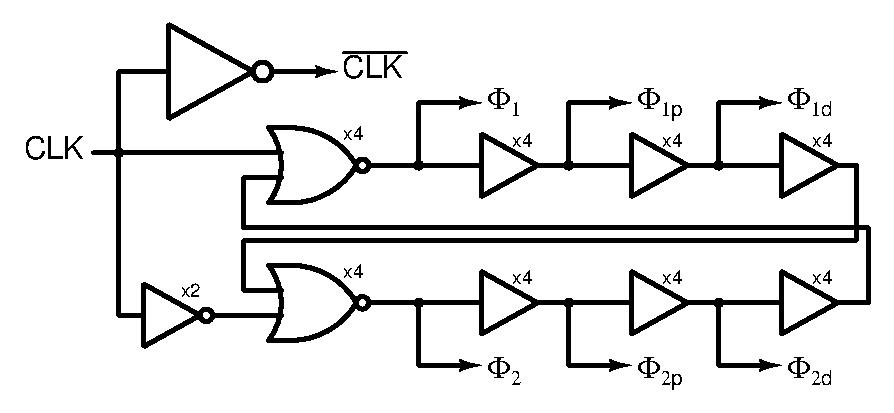
\includegraphics[width=0.75\textwidth]{Chapter4/Figs/non-overlapp.ps}
	\caption{Two-phase non overlapping generator circuit}
	\label{fig:non-ov}
\end{figure}

In such topology, buffers define the driving capability of phase generator. In many applications in order to maximize the available settling time for the circuit, the phase's widths are widened by minimizing non-overlapping duration. Hence, the number of logic gates used in the clock generator is normally minimized, also reducing the accumulated jitter. 

For the bottom sampling, both \(\Phi_1\) and \(\Phi_{1d}\) drive sampling switches. In this regard, the delay between those two shall be minimal to allow the maximum sampling time with a delay bigger than the commutation time of the bottom switch. By using buffers for medium strength (x4), the delay introduced admits a maximum of 400 ps and a minimum of 200 ps.
\paragraph{Switches command signal driver}
\label{sec:dig-driver}

As discussed earlier, the simultaneity of turning off switches prevents ambiguity in the sampled value when the settling time is limited and the non-overlapping time is short. In order to make transition crossing the most possible around half the power supply for complementary switches, the driver of the \figurename~\ref{fig:dig-driver-ideal} is ideally used. As the inverter and the transmission gate exhibits both a small propagation delay, they almost compensate for each other. In fact, process variation generates different trip point for inverters while the equivalent resistance of transmission barely changes in comparison. The mismatch between the RC settling of the transmission gate and the pseudo-RC settling of inverters becomes ever more prominent. 

\begin{figure}[htp]
	\centering
	\begin{subfigure}[b]{0.48\textwidth}
		\centering
		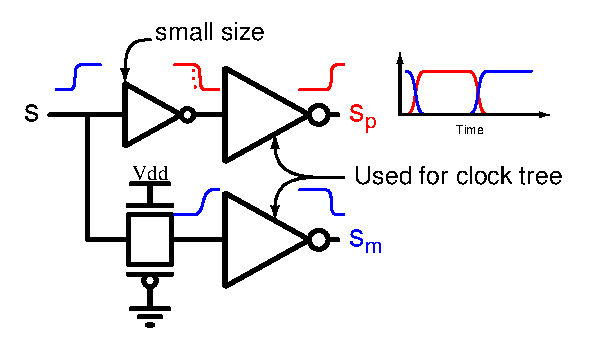
\includegraphics[width=\textwidth]{Chapter4/Figs/digital-driver.ps}
		\subcaption{ideal driver}
		\label{fig:dig-driver-ideal}
	\end{subfigure}
	\begin{subfigure}[b]{0.48\textwidth}
		\centering
		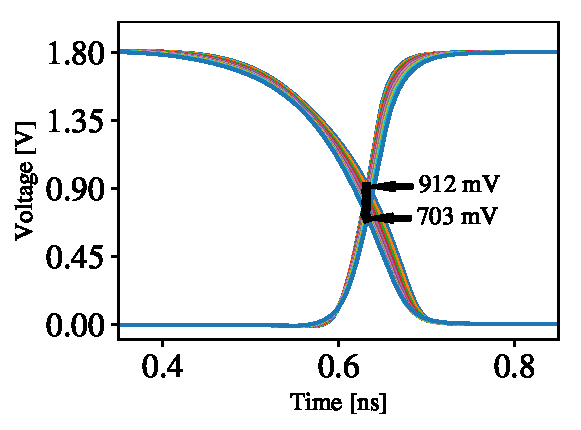
\includegraphics[width=\textwidth]{Chapter4/Figs/crossing-driver-with-tgate.pdf}
		\subcaption{crossing over temperature}
		\label{fig:dig-driver-crossing}
	\end{subfigure}
	\caption{Digital driver to ensure PMOS and NMOS command signal $S_p/S_m$ transition crossing around half the power supply voltage}
	\label{fig:dig-driver}
\end{figure}

For a minimal size inverter, good results are given without the transmission gate as depicted by \figurename~\ref{fig:dig-driver-crossing}. In a typical corner over temperature, the variation of the crossing point is 300 ps for a capacitive load that analog switches represent. Crossings between the PMOS and the NMOS command signals are in the 600-725 mV range over the temperature range. Taking into account the process variation, this range enlarges to 490-850 mV. With the transmission gate, the delay for low-to high variation is compensated. Taking into account the process variation, this range enlarges to 700-1150 mV. In comparison, the range suffers from a greater process variation given by the transmission gate equivalent resistance while the range is centred around half the power supply voltage. Furthermore crossings occurs at almost the same time over temperature. For this last reason, the version using transmission gate is preferred.
\paragraph{Relaxed comparator constraints}

Analog constraints undergo large variation with process alteration and increasing temperature. In this regard, the digital should respect these constraints, but can also relieve them. As an example, the transition frequency of a single transistor as a sensitivity of about 2000 ppm/\(\degree \)C. This is equivalent to say from -40\(\degree \)C to 175\(\degree \)C that the speed is reduced by 35 \%. For the sake of simplicity, let us assume comparators follows the same trend over temperature. As the differential input is getting closer to zero, the delay increase. While in most of the case the decision is made within the non-overlapping time, this is not the case with this design. This is done in order to reduce the probability of a metastable state, or more generally to prevent latch output transition at the time the digital is applying the feedback voltage.
\begin{figure}[htp]
	\centering
	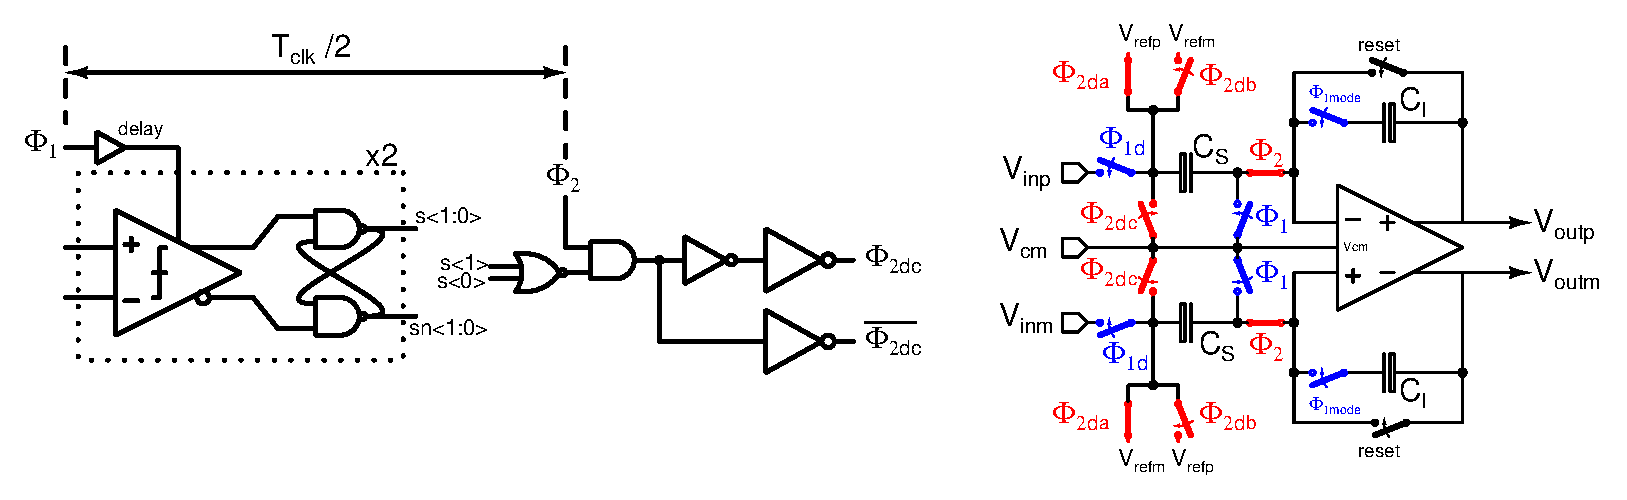
\includegraphics[width=0.75\textwidth]{Chapter4/Figs/comp-timing-isd.ps}
	\caption{Comparator relaxed constraints by appropriate scheduling}
	\label{fig:comp-timing}
\end{figure}

\figurename~\ref{fig:comp-timing} depicts the scheduling of the comparator decision in order to apply the correct voltage feedback. As the second clock phase settles the input voltage of the quantizer, the comparator makes a decision in less than 1 ns after. The decision made toggle the nand-RS-latch to generate the appropriate feedback selector signal. In the case of the critical path, a single gate generates the signal. The following AND gate makes the results only available for the next second phase of the clock. Therefore, between the beginning of the settling of input voltages to compare and the available result signal, there is \(T_{clk}/2-T_{delay}-T_{RSLatch}-T_{nor}-T_{setup}\) for the comparator.

In summary, the first stage Incremental-$\Delta\Sigma$ heavily relies on the performance of the integrator. The design from the top-level down to switches' transistors have been considered to reduce the INL drop due to parasitics, coupling, charge trapped and mismatches. From a system point of view, the fully differential structure limits the impact of clock coupling, charge injections and mismatches. With a parasitic insensitive topology, the parasitic can be disregarded for the design as the switches command signals are non-overlapping and limits charge injections. However, only partial specification have been given for the OTA not discussed yet.
Connected to the integrator, the 3-levels switched capacitor quantizer limits the swing of the residue by making the decision of the feedback to apply. Being the interface between comparators and the integrator, the offset introduced by mismatch in capacitors sums with the offset of comparators. The excursion of the residue takes into account the disturbance to be processed by the following stage: the Algorithmic.
\clearpage
	 
\subsection{Algorithmic}                    % section 5.2
\textbf{\textcolor{black}{principle:}}
The principle of the Algorithmic conversion lies in the successive amplification of the estimation error. Made out of an ADC-DAC chain to estimate the input voltage, the error is then amplified by an arbitrary factor $a$ before the recycle of this error as the new input of this converter.

For its first clock cycle, this stage sample the residue of the previous stage. Herein the previous stage residue is named \(V_{\rm in}\) for clarity as represented in \figurename~\ref{fig:algo-alone-clk-cycle}. After the comparator makes a decision, either \(+bV_{\rm ref} \), or 0, or \(-bV_{\rm ref} \) is added to the amplified input signal. The output of the adder is the part of the input that has not yet been quantized and is called the residue. Here \(a\) denotes the gain applied to the residue between comparator decisions and is called the residue gain. In later cycles, the input switch is always in the up position, and the residue is sent back to the comparator for further quantization as in \figurename~\ref{fig:algo-alone-std-clk-cycle}.

\begin{figure}[htp]
	\centering
	\begin{subfigure}[b]{0.48\textwidth}
		\centering
		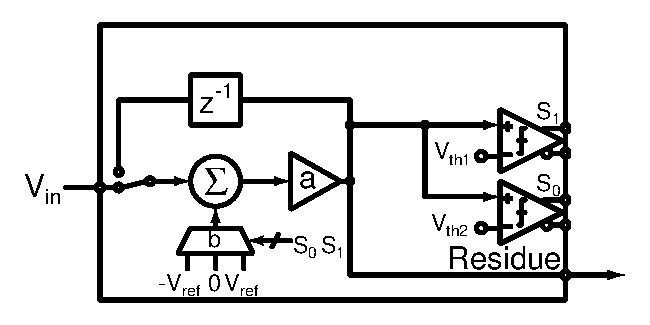
\includegraphics[width=\textwidth]{Chapter4/Figs/algorithmic-principle-new_sample.ps}
		\subcaption{first clock cycle}
		\label{fig:algo-alone-reset-clk-cycle}
	\end{subfigure}
	\begin{subfigure}[b]{0.48\textwidth}
		\centering
		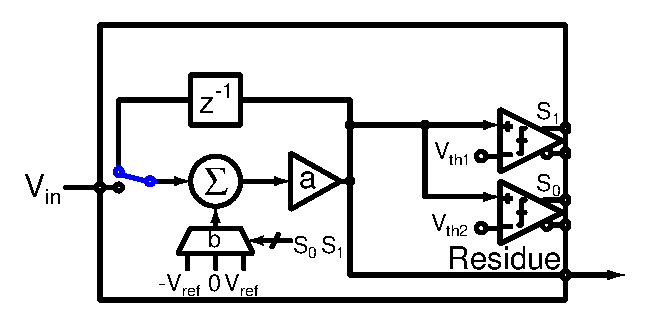
\includegraphics[width=\textwidth]{Chapter4/Figs/algorithmic-principle.ps}
		\subcaption{following clock cycles}
		\label{fig:algo-alone-std-clk-cycle}
	\end{subfigure}
	% \begin{subfigure}[b]{0.32\textwidth}
	% 	\centering
	% 	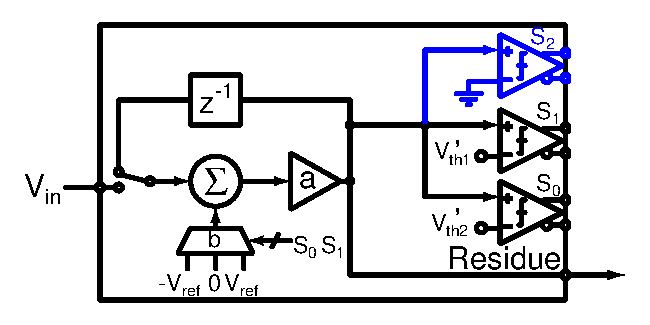
\includegraphics[width=\textwidth]{Chapter4/Figs/algorithmic-principle-last.ps}
	% 	\subcaption{last clock cycle}
	% 	\label{fig:algo-alone-last-clk-cycle}
	% \end{subfigure}
	\caption{3-level algorithmic stage operation}
	\label{fig:algo-alone-clk-cycle}
\end{figure}

\textbf{\textcolor{black}{limitations from analog error amplified and on residue:}}
A common implementation of the algorithmic converter is by building the stage around a Flip-Around Multiplying DAC (FA-MDAC) composed of two capacitors and one amplifier. While a simple differential pair is a valid amplifier to operate under low-supply condition, as the resolution increased the gain of the amplifier shall drastically increase too. Indeed, at each clock cycle the FA-MDAC recycles its inner self error. To achieve high gain amplifier by stacking transistors the output swing is thus limited and non-linearity occurs. Therefore, medium to high resolution algorithmic ADC require a digital compensation or an adjustment of its residue curve.

\textbf{\textcolor{black}{resolution enhancement with interstage gain:}}
Besides this, the residue of the first stage is within the $\pm V_{\rm ref}/2$ range. With a SAR following this stage, an increase of this stage residue can be converted. In consequence, the resolution of the ADC can be enhanced by the introduction of an interstage gain to amplify the residue of the first stage. The benefits and limitations of an interstage gain will be discussed later in this section.

\textbf{\textcolor{black}{resolution enhancement and threshold change:}}
In addition to that, the architecture proposal discussed in section~\ref{sec:selected-topology} consists in turning the estimation of the error provided by the last clock cycle into the first bits of the SAR. Depending on the adjustment of the residue curve, threshold voltages of the quantizer change in the last cycle to \(\pm V_{\rm ref}/2\). Depicted by \figurename~\ref{fig:sar-first-bits-from-algo}, during this last clock cycle, a third comparator is used to give the sign of the residue. The output of the comparison results in the expected first step perform by a SAR\@. The threshold change matching the threshold of the second step of the SAR, the combined the outputs of the three comparators provide the quadrant of the residue. This digital information will be used by the third stage of the converter right after the sampling phase to perform its third comparison.

\begin{figure}[htp]
	\centering
	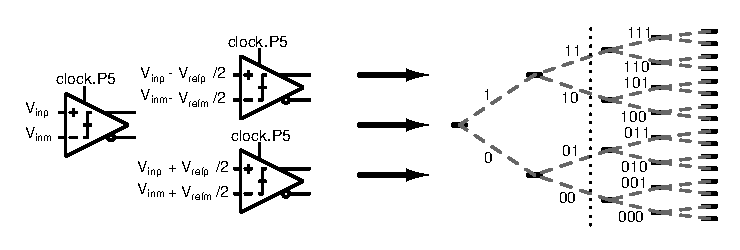
\includegraphics[width=\textwidth]{Chapter4/Figs/algo_sar_first_bits.ps}
	\caption{Principle to enhance the number of extracted bits by using on extra comparator inside the algorithmic stage to perform the two first steps of a charge-redistribution SAR}
	\label{fig:sar-first-bits-from-algo}
\end{figure}

\textbf{\textcolor{black}{solutions (residue constrained with a 1.5-bit quantizer):}}
Expecting a digital calibration of mismatch compensation, the adjustment of the residue curve provides the necessary margin to achieve medium to high resolution with an algorithmic ADC\@. With a transfer function of the form $V_{\rm residue}[n+1] = a V_{\rm residue}[n] \pm b V_{\rm ref}$, the two parameters $a$ and $b$ can be tuned.

If the residue gain \(a = 2\), N-bit conversion requires N clock cycles and the output code is simply raw output bits of the comparator shifted and added. Reducing the residue gain increases the number of required clock cycles, but also introduces redundancy, allowing ADC non-linearity from the SHA charge injection, comparator offset, and OTA offset to be avoided~\cite{Lewis1987}. However, the ADC output cannot be calculated by a simple bit shift and addition. So, we decide to keep the residue gain \(a = 2\).

Thus, redundancy is introduced via a 1.5-bit quantizer to relax the requirements on the offset of the comparator and the amplifier. As performed in the design of the first stage, we thus constrain the residue within the desired range by tuning the parameter $b$.

Classical algorithmic converters use threshold voltages equal to \(\pm V_{\rm ref}/4\) and a feedback gain \(b = 1\) such that the residue is depicted in \figurename~\ref{fig:algo-21}~\cite{Brooks2009,Naderi2017}. In this case, the sub-ADC is resilient to large comparator and amplifier offset by demonstrating a large margin between the \(\pm V_{\rm ref}\) limits and the maximum of the residue curve. Unfortunately, such error on the first stage increase the input voltage range, which results in a range overflow. Let us suppose we do not want to exceed $\pm V_{\rm ref}/2$. For the case represented in \figurename~\ref{fig:algo-21}, an offset on the comparator of the first stage will increase the input voltage to $\pm V_{\rm ref}/2+V_{\rm offset}$. The error committed on the residue range is twice $V_{\rm offset}$. With an interstage gain envisioned, the effect could be catastrophic: the residue could exceed $\pm V_{\rm ref}$ range leading to missing codes.

By using the general shape of the residue represented in \figurename~\ref{fig:algo-general}, the residue is bounded by an appropriate choice of threshold voltages and the feedback gain \(b\). Let us suppose the desired residue is symmetrical around 0 and based on the a system study we required a tolerance of \(l/a\) for charge injection, comparator offset, OTA offset. Hence, the extrema of the residue curve is \(l = aV_{\rm th2} = aV_{\rm th1}+bV_{\rm ref} = -aV_{\rm th1} = -aV_{\rm th2}+bV_{\rm ref}\). From these equations, the threshold voltages are given as 

\begin{equation}
V_{\rm th2} = l/a = -V_{\rm th1}
\end{equation}
while the feedback gain b is given by 

\begin{equation}
b = \frac{2l}{V_{\rm ref}}
\end{equation}

From a robustness point of view, such design handles input range overflow since the input values which makes the residue crossing \(\pm V_{\rm ref}\) are \(\pm \frac{1+b}{a}V_{\rm ref}\). For the conventional design \(a=2, b=1, V_{th}=\pm V_{\rm ref}/4\), the maximum input range is \(\pm V_{\rm ref}\). For a tolerance of 10\% of \(V_{\rm ref}\) for offset and charge injection, or l = 0.8 \(V_{\rm ref}\), the input range extends to \(\pm 1.3 V_{\rm ref}\). From the design of the first stage and considering a precise inter-stage gain of 2, the tolerance for the offset on the first stage is 15\% of \(V_{\rm ref}\). 

\begin{figure}[htp]
	\centering
	\begin{subfigure}[b]{0.32\textwidth}
		\centering
		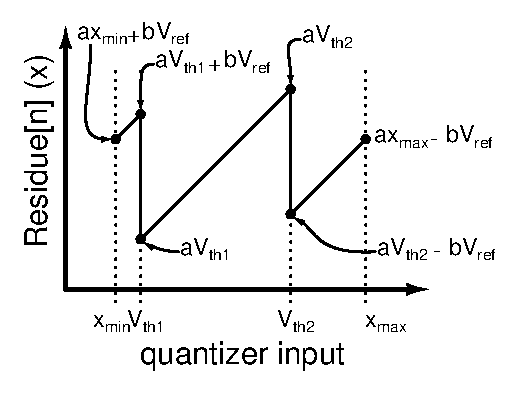
\includegraphics[width=\textwidth]{Chapter4/Figs/3-levels-pattern-algo.ps}
		\subcaption{first clock cycle}
		\label{fig:algo-general}
	\end{subfigure}
	\begin{subfigure}[b]{0.32\textwidth}
		\centering
		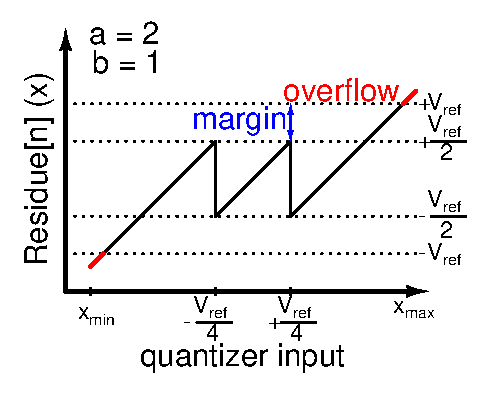
\includegraphics[width=\textwidth]{Chapter4/Figs/3-levels-pattern-algo-2-1.ps}
		\subcaption{following clock cycles}
		\label{fig:algo-21}
	\end{subfigure}
	\begin{subfigure}[b]{0.32\textwidth}
		\centering
		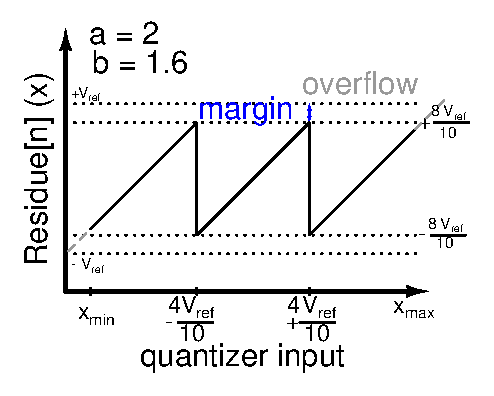
\includegraphics[width=\textwidth]{Chapter4/Figs/3-levels-pattern-algo-2-1_6.ps}
		\subcaption{last clock cycle}
		\label{fig:algo-21-6}
	\end{subfigure}
	\caption{3-levels algorithmic stage operation as an optimization for robustness}
	\label{fig:algo-quantizer}
\end{figure}

This slightly novel approach allows to find the best compromise between performance and sensitivity to offset by changing the feedback gain. The threshold voltages required by a 1.5-bit quantizer vary accordingly as a quarter of the feedback gain. With a feedback gain equals to 1, we found back the conventional design. Of course, the residue range changing with $b$, the possible interstage gain depends on the feedback gain. To keep performance high, with a small area footprint, the optimization of the residue curve should consider the design of the interstage gain.

	\subsubsection{Gain Stage}              % section 5.2.2
	\label{sec:algo_gain_stage}
Based on a common Flip-Around Multiplying DAC (FA-MDAC) represented in \figurename~\ref{fig:algo-mdac}, the input is sampled by \(C_S+C_F\) in a the clock phase while in the second clock phase the reference is subtract only on \(C_S\). This way, the closed-loop gain is defined by a ratio of capacitor \(1+C_S/C_F\). The capacitor ratio mismatch is well controlled, both the charge subtraction weighted by \(C_S/C_F\) and the gain are well-controlled. By default, this architecture fits the conventional residue gain and feedback gain values of respectively 2 and 1.

\begin{figure}[htp]
	\centering
	\begin{subfigure}[b]{0.4\textwidth}
		\centering
		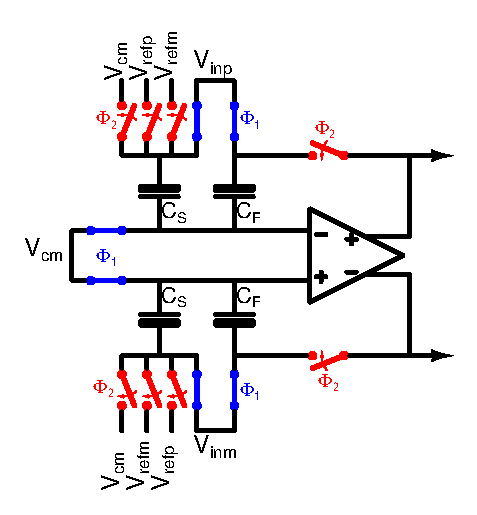
\includegraphics[width=\textwidth]{Chapter4/Figs/algorithmic-mdac-phi1.ps}
		\subcaption{first clock phase}
		\label{fig:algo-mdac-phi1}
	\end{subfigure}
	\begin{subfigure}[b]{0.4\textwidth}
		\centering
		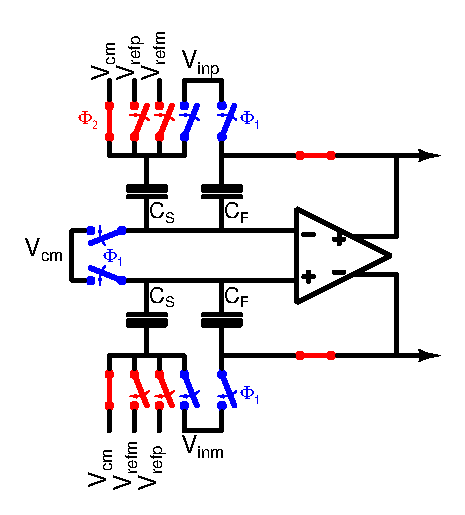
\includegraphics[width=\textwidth]{Chapter4/Figs/algorithmic-mdac-phi2.ps}
		\subcaption{second clock phase}
		\label{fig:algo-mdac-phi2}
	\end{subfigure}
	\caption{Standard Flip-Around MDAC operation for the algorithmic implementation}
	\label{fig:algo-mdac}
\end{figure}

\textbf{\textcolor{black}{inter stage gain:}}
The second tuning relates to the inter-stage gain. As only the sampling of the first stage residue shall be multiplied by a factor of two, an extra capacitance \(C_G\) is mandatory. As represented in \figurename~\ref{fig:algo-Cg-phi1}, during the sampling phase the capacitor \(C_G\) is connected to the inputs of the OTA and the first stage residue for the sampling. Then illustrated by \figurename~\ref{fig:algo-Cg-phi2}, till to the end of the sample conversion the latter is connected to the inputs of the OTA and the common-mode voltage \(V_{\rm cm}\).

\begin{figure}[htp]
	\centering
	\begin{subfigure}[b]{0.45\textwidth}
		\centering
		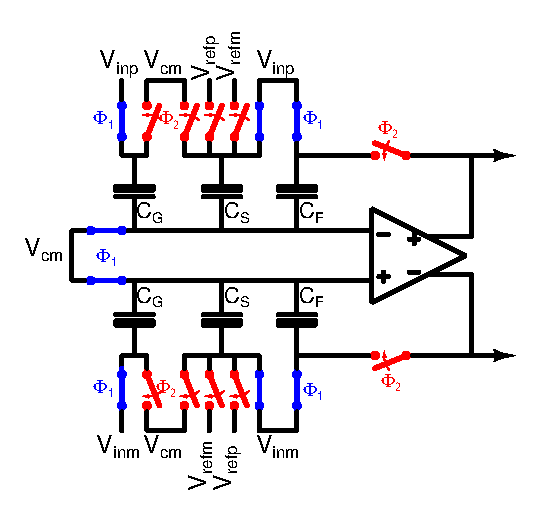
\includegraphics[width=\textwidth]{Chapter4/Figs/algorithmic-Cg-phi1.ps}
		\subcaption{first clock phase}
		\label{fig:algo-Cg-phi1}
	\end{subfigure}
	\begin{subfigure}[b]{0.45\textwidth}
		\centering
		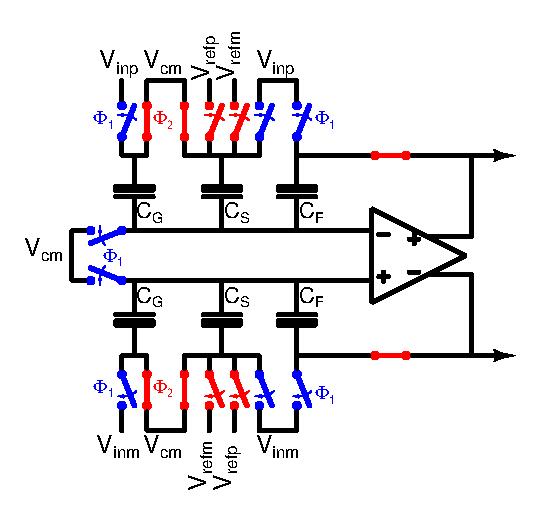
\includegraphics[width=\textwidth]{Chapter4/Figs/algorithmic-Cg-phi2.ps}
		\subcaption{second clock phase}
		\label{fig:algo-Cg-phi2}
	\end{subfigure}
	\caption{Flip-Around MDAC operation during the first clock cycle only for the implementation of interstage gain}
	\label{fig:algo-mdac-cg}
\end{figure}

Over the first clock cycle, the charges stored in the system for an amplifier gain $A$ are
\begin{align}
Q_{11p} &= \left(C_G+C_S+C_F \right) \left( V_{\rm inp}[n-1] - V_{\rm cm} \right)\\
Q_{12p} &= \left(C_S \right) \left( V_{\rm ref}b_i[n-1] - V^{-}[n] \right) + C_G \left(V_{\rm cm}-V^{-}[n] \right)  + C_F \left(V_{\rm op}[n]-V^{-}[n] \right) \\
Q_{11m} &= \left(C_G+C_S+C_F \right) \left( V_{\rm inm}[n-1] - V_{\rm cm} \right) \\
Q_{12m} &= \left(C_S \right) \left( V_{\rm ref}b_i[n-1] - V^{+}[n] \right) + C_G \left(V_{\rm cm}-V^{+}[n] \right)  + C_F \left(V_{\rm om}[n]-V^{+}[n] \right)
\end{align}

which results in a differential output voltage following 
\begin{equation}
	V_{\rm out}[n] = \frac{C_G+C_S+C_F}{C_F+\frac{C_G+C_S+C_F}{A}} V_{\rm in}[n-1] - \frac{C_S}{C_F+\frac{C_G+C_S+C_F}{A}} V_{\rm ref}b_i[n-1]
\end{equation}

Then, the gain capacitor being always connected to the $V_{\rm cm}$, the transfer function for following clock cycles is 
\begin{equation}
	V_{\rm out}[n] = \frac{C_S+C_F}{C_F+\frac{C_G+C_S+C_F}{A}} V_{\rm in}[n-1] - \frac{C_S}{C_F+\frac{C_G+C_S+C_F}{A}} V_{\rm ref}b_i[n-1]
\end{equation}

We deduce the interstage gain as the ratio of input gain between the first and the following clock cycles, to wit, $1+frac{C_G}{C_S+C_F}$.  In this configuration, the gain capacitor is not disconnected to prevent a switch injecting thermal noise on the input of the amplifier, and to simplify the digital calibration as the feedback gain is constant.

\textbf{\textcolor{black}{feedback gain:}}
To optimize the feedback gain $b$, either new references can be generated for this stage, or an extra capacitor can be charged and connected. The change of reference voltages only for this stage is not recommended as extra circuitry is required which could exhibit a temperature variation in opposition to the first stage references. In this case, the accuracy of the ADC is compromised.

To the contrary, a capacitor ratio based design based on capacitance experiences a reduced alteration and good variation over temperature and process. As the feedback gain of a conventional FA-MDAC has been set to \(C_S/C_F = 1\), only an extra fraction of \(V_{\rm ref}\) capacitance is required. Considering a design with unit capacitors, both the sampling and the feedback capacitance could be Q units. \figurename~\ref{fig:algo-mdac-cb} highlights the extra capacitance \(C_B\) of P units connected between the OTA inputs and the feedback voltage applied to \(C_S\) in order to bring charges in the amounts of \(C_B/C_F = P/Q\) of \(V_{\rm ref}\). During the sampling phase on \(C_S\) and \(C_F\), this \(C_B\) capacitor is reset by connecting its plates to the common-mode voltage \(V_{\rm cm}\).

For instance, a feedback gain $b = 1.6$ need an extra 0.6 times \(V_{\rm ref}\). This ratio being equal to 3/5, one set $C_S = C_F = 5 C_0$ with $C_B = 3 C_0$. And for a feedback gain $b = 1.25$, $C_S = C_F = 4 C_0$ and $C_B = C_0$. In general, a feedback gain $b$ in the form 1+P/Q requires 2Q unit capacitors for $C_S$ and $C_F$ and P unit capacitors for $C_B$. To reduce the area, Q should be the smallest possible.

\begin{figure}[htp]
	\centering
	\begin{subfigure}[b]{0.45\textwidth}
		\centering
		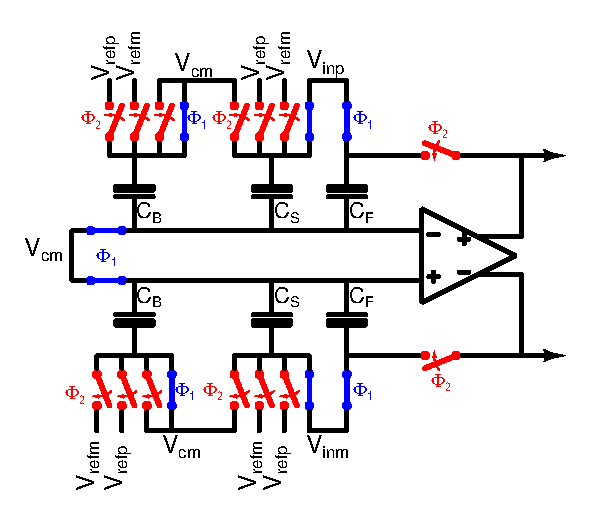
\includegraphics[width=\textwidth]{Chapter4/Figs/algorithmic-Cb-phi1.ps}
		\subcaption{first clock phase}
		\label{fig:algo-mdac-phi1}
	\end{subfigure}
	\begin{subfigure}[b]{0.45\textwidth}
		\centering
		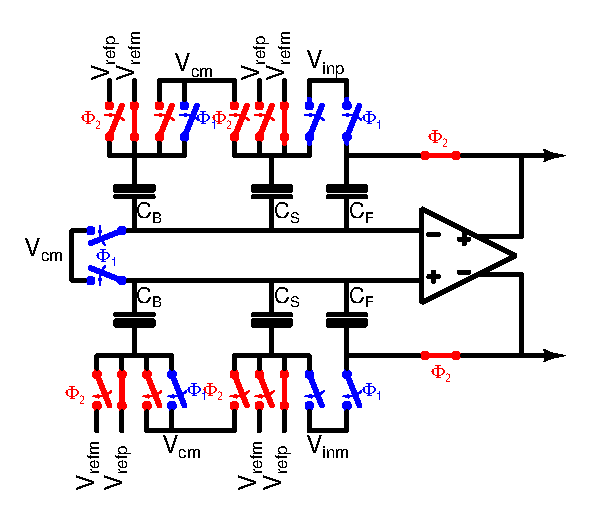
\includegraphics[width=\textwidth]{Chapter4/Figs/algorithmic-Cb-phi2.ps}
		\subcaption{second clock phase}
		\label{fig:algo-mdac-phi2}
	\end{subfigure}
	\caption{Flip-Around MDAC operation for the algorithmic implementation of arbitrary feedback gain}
	\label{fig:algo-mdac-cb}
\end{figure}

To estimate the error by combining the modification of the interstage gain and the feedback gain, over the first clock cycle, the charges stored in the system are
\begin{align}
Q_{11p} &= \left(C_G+C_S+C_F \right) \left( V_{\rm inp}[n-1] - V_{\rm cm} \right) + C_B \left(V_{\rm cm}-V_{\rm cm} \right) \\
Q_{12p} &= \left(C_S+C_B \right) \left( V_{\rm ref}b_i[n-1] - V^{-}[n] \right) + C_G \left(V_{\rm cm}-V^{-}[n] \right)  + C_F \left(V_{\rm op}[n]-V^{-}[n] \right) \\
Q_{11m} &= \left(C_G+C_S+C_F \right) \left( V_{\rm inm}[n-1] - V_{\rm cm} \right) + C_B \left(V_{\rm cm}-V_{\rm cm} \right) \\
Q_{12m} &= \left(C_S+C_B \right) \left( V_{\rm ref}b_i[n-1] - V^{+}[n] \right) + C_G \left(V_{\rm cm}-V^{+}[n] \right)  + C_F \left(V_{\rm om}[n]-V^{+}[n] \right) 
\end{align}
which results in a differential output voltage following 
\begin{equation}
	V_{\rm out}[n] = \frac{C_G+C_S+C_F}{C_F+\frac{C_B+C_G+C_S+C_F}{A}} V_{\rm in}[n-1] - \frac{C_S+C_B}{C_F+\frac{C_B+C_G+C_S+C_F}{A}} V_{\rm ref}b_i[n-1]
\end{equation}

Then, in the same manner, the differential output voltage for following clock cycles is
\begin{equation}
	V_{\rm out}[n] = \frac{C_S+C_F}{C_F+\frac{C_B+C_G+C_S+C_F}{A}} V_{\rm in}[n-1] - \frac{C_S+C_B}{C_F+\frac{C_B+C_G+C_S+C_F}{A}} V_{\rm ref}b_i[n-1]
\end{equation}

\textbf{\textcolor{black}{optimization of ratio:}}
For the sake of clarity, we define the interstage gain of \(g = 1+C_G/(2C_F)\) and a feedback gain of \(b = 1+C_B/C_F\), after N clock cycle the estimated error for the same output code is
\begin{equation}
	error[N] = g \times 2^N \left(1-{\left(\frac{1}{1+\frac{2g+b-1}{A}} \right)}^N \right) V_{\rm in} - b \times \sum_{i=0}^{N-1}{2^i\left(1-{\left(\frac{1}{1+\frac{2g+b-1}{A}} \right)}^{i+1} \right)} V_{\rm ref}
\end{equation}

From this equation, the minimum gain of the amplifier can be calculated as we already know the maximum excursion of this sub-ADC input range: \(\pm V_{\rm ref}/2\). It is also worth to note the impact of the feedback and the interstage gain on the error for a given DC Gain of the OTA\@. \figurename~\ref{fig:algo-cb-impact} depicts the error at the end of the sample conversion for different values of the feedback gain \(b\). In order to preserve the symmetry of the residue curve the threshold voltage of the 3-levels quantizer shall be \(\pm b/4 V_{\rm ref}\). In turn the output range is delimited by \(\pm b/2 V_{\rm ref}\). 

\begin{figure}[htp]
	\centering
	\begin{subfigure}[b]{0.45\textwidth}
		\centering
		\resizebox{\textwidth}{!}{
			%% Creator: Matplotlib, PGF backend
%%
%% To include the figure in your LaTeX document, write
%%   \input{<filename>.pgf}
%%
%% Make sure the required packages are loaded in your preamble
%%   \usepackage{pgf}
%%
%% Figures using additional raster images can only be included by \input if
%% they are in the same directory as the main LaTeX file. For loading figures
%% from other directories you can use the `import` package
%%   \usepackage{import}
%% and then include the figures with
%%   \import{<path to file>}{<filename>.pgf}
%%
%% Matplotlib used the following preamble
%%   \usepackage{fontspec}
%%   \setmainfont{DejaVu Serif}
%%   \setsansfont{DejaVu Sans}
%%   \setmonofont{DejaVu Sans Mono}
%%
\begingroup%
\makeatletter%
\begin{pgfpicture}%
\pgfpathrectangle{\pgfpointorigin}{\pgfqpoint{3.836166in}{2.848953in}}%
\pgfusepath{use as bounding box, clip}%
\begin{pgfscope}%
\pgfsetbuttcap%
\pgfsetmiterjoin%
\definecolor{currentfill}{rgb}{1.000000,1.000000,1.000000}%
\pgfsetfillcolor{currentfill}%
\pgfsetlinewidth{0.000000pt}%
\definecolor{currentstroke}{rgb}{1.000000,1.000000,1.000000}%
\pgfsetstrokecolor{currentstroke}%
\pgfsetdash{}{0pt}%
\pgfpathmoveto{\pgfqpoint{0.000000in}{0.000000in}}%
\pgfpathlineto{\pgfqpoint{3.836166in}{0.000000in}}%
\pgfpathlineto{\pgfqpoint{3.836166in}{2.848953in}}%
\pgfpathlineto{\pgfqpoint{0.000000in}{2.848953in}}%
\pgfpathclose%
\pgfusepath{fill}%
\end{pgfscope}%
\begin{pgfscope}%
\pgfsetbuttcap%
\pgfsetmiterjoin%
\definecolor{currentfill}{rgb}{1.000000,1.000000,1.000000}%
\pgfsetfillcolor{currentfill}%
\pgfsetlinewidth{0.000000pt}%
\definecolor{currentstroke}{rgb}{0.000000,0.000000,0.000000}%
\pgfsetstrokecolor{currentstroke}%
\pgfsetstrokeopacity{0.000000}%
\pgfsetdash{}{0pt}%
\pgfpathmoveto{\pgfqpoint{0.577266in}{0.575369in}}%
\pgfpathlineto{\pgfqpoint{3.654570in}{0.575369in}}%
\pgfpathlineto{\pgfqpoint{3.654570in}{2.731453in}}%
\pgfpathlineto{\pgfqpoint{0.577266in}{2.731453in}}%
\pgfpathclose%
\pgfusepath{fill}%
\end{pgfscope}%
\begin{pgfscope}%
\pgfsetbuttcap%
\pgfsetroundjoin%
\definecolor{currentfill}{rgb}{0.000000,0.000000,0.000000}%
\pgfsetfillcolor{currentfill}%
\pgfsetlinewidth{0.803000pt}%
\definecolor{currentstroke}{rgb}{0.000000,0.000000,0.000000}%
\pgfsetstrokecolor{currentstroke}%
\pgfsetdash{}{0pt}%
\pgfsys@defobject{currentmarker}{\pgfqpoint{0.000000in}{-0.048611in}}{\pgfqpoint{0.000000in}{0.000000in}}{%
\pgfpathmoveto{\pgfqpoint{0.000000in}{0.000000in}}%
\pgfpathlineto{\pgfqpoint{0.000000in}{-0.048611in}}%
\pgfusepath{stroke,fill}%
}%
\begin{pgfscope}%
\pgfsys@transformshift{0.577266in}{0.575369in}%
\pgfsys@useobject{currentmarker}{}%
\end{pgfscope}%
\end{pgfscope}%
\begin{pgfscope}%
\pgftext[x=0.577266in,y=0.478146in,,top]{\sffamily\fontsize{12.000000}{14.400000}\selectfont \(\displaystyle 65\)}%
\end{pgfscope}%
\begin{pgfscope}%
\pgfsetbuttcap%
\pgfsetroundjoin%
\definecolor{currentfill}{rgb}{0.000000,0.000000,0.000000}%
\pgfsetfillcolor{currentfill}%
\pgfsetlinewidth{0.803000pt}%
\definecolor{currentstroke}{rgb}{0.000000,0.000000,0.000000}%
\pgfsetstrokecolor{currentstroke}%
\pgfsetdash{}{0pt}%
\pgfsys@defobject{currentmarker}{\pgfqpoint{0.000000in}{-0.048611in}}{\pgfqpoint{0.000000in}{0.000000in}}{%
\pgfpathmoveto{\pgfqpoint{0.000000in}{0.000000in}}%
\pgfpathlineto{\pgfqpoint{0.000000in}{-0.048611in}}%
\pgfusepath{stroke,fill}%
}%
\begin{pgfscope}%
\pgfsys@transformshift{1.192727in}{0.575369in}%
\pgfsys@useobject{currentmarker}{}%
\end{pgfscope}%
\end{pgfscope}%
\begin{pgfscope}%
\pgftext[x=1.192727in,y=0.478146in,,top]{\sffamily\fontsize{12.000000}{14.400000}\selectfont \(\displaystyle 70\)}%
\end{pgfscope}%
\begin{pgfscope}%
\pgfsetbuttcap%
\pgfsetroundjoin%
\definecolor{currentfill}{rgb}{0.000000,0.000000,0.000000}%
\pgfsetfillcolor{currentfill}%
\pgfsetlinewidth{0.803000pt}%
\definecolor{currentstroke}{rgb}{0.000000,0.000000,0.000000}%
\pgfsetstrokecolor{currentstroke}%
\pgfsetdash{}{0pt}%
\pgfsys@defobject{currentmarker}{\pgfqpoint{0.000000in}{-0.048611in}}{\pgfqpoint{0.000000in}{0.000000in}}{%
\pgfpathmoveto{\pgfqpoint{0.000000in}{0.000000in}}%
\pgfpathlineto{\pgfqpoint{0.000000in}{-0.048611in}}%
\pgfusepath{stroke,fill}%
}%
\begin{pgfscope}%
\pgfsys@transformshift{1.808187in}{0.575369in}%
\pgfsys@useobject{currentmarker}{}%
\end{pgfscope}%
\end{pgfscope}%
\begin{pgfscope}%
\pgftext[x=1.808187in,y=0.478146in,,top]{\sffamily\fontsize{12.000000}{14.400000}\selectfont \(\displaystyle 75\)}%
\end{pgfscope}%
\begin{pgfscope}%
\pgfsetbuttcap%
\pgfsetroundjoin%
\definecolor{currentfill}{rgb}{0.000000,0.000000,0.000000}%
\pgfsetfillcolor{currentfill}%
\pgfsetlinewidth{0.803000pt}%
\definecolor{currentstroke}{rgb}{0.000000,0.000000,0.000000}%
\pgfsetstrokecolor{currentstroke}%
\pgfsetdash{}{0pt}%
\pgfsys@defobject{currentmarker}{\pgfqpoint{0.000000in}{-0.048611in}}{\pgfqpoint{0.000000in}{0.000000in}}{%
\pgfpathmoveto{\pgfqpoint{0.000000in}{0.000000in}}%
\pgfpathlineto{\pgfqpoint{0.000000in}{-0.048611in}}%
\pgfusepath{stroke,fill}%
}%
\begin{pgfscope}%
\pgfsys@transformshift{2.423648in}{0.575369in}%
\pgfsys@useobject{currentmarker}{}%
\end{pgfscope}%
\end{pgfscope}%
\begin{pgfscope}%
\pgftext[x=2.423648in,y=0.478146in,,top]{\sffamily\fontsize{12.000000}{14.400000}\selectfont \(\displaystyle 80\)}%
\end{pgfscope}%
\begin{pgfscope}%
\pgfsetbuttcap%
\pgfsetroundjoin%
\definecolor{currentfill}{rgb}{0.000000,0.000000,0.000000}%
\pgfsetfillcolor{currentfill}%
\pgfsetlinewidth{0.803000pt}%
\definecolor{currentstroke}{rgb}{0.000000,0.000000,0.000000}%
\pgfsetstrokecolor{currentstroke}%
\pgfsetdash{}{0pt}%
\pgfsys@defobject{currentmarker}{\pgfqpoint{0.000000in}{-0.048611in}}{\pgfqpoint{0.000000in}{0.000000in}}{%
\pgfpathmoveto{\pgfqpoint{0.000000in}{0.000000in}}%
\pgfpathlineto{\pgfqpoint{0.000000in}{-0.048611in}}%
\pgfusepath{stroke,fill}%
}%
\begin{pgfscope}%
\pgfsys@transformshift{3.039109in}{0.575369in}%
\pgfsys@useobject{currentmarker}{}%
\end{pgfscope}%
\end{pgfscope}%
\begin{pgfscope}%
\pgftext[x=3.039109in,y=0.478146in,,top]{\sffamily\fontsize{12.000000}{14.400000}\selectfont \(\displaystyle 85\)}%
\end{pgfscope}%
\begin{pgfscope}%
\pgfsetbuttcap%
\pgfsetroundjoin%
\definecolor{currentfill}{rgb}{0.000000,0.000000,0.000000}%
\pgfsetfillcolor{currentfill}%
\pgfsetlinewidth{0.803000pt}%
\definecolor{currentstroke}{rgb}{0.000000,0.000000,0.000000}%
\pgfsetstrokecolor{currentstroke}%
\pgfsetdash{}{0pt}%
\pgfsys@defobject{currentmarker}{\pgfqpoint{0.000000in}{-0.048611in}}{\pgfqpoint{0.000000in}{0.000000in}}{%
\pgfpathmoveto{\pgfqpoint{0.000000in}{0.000000in}}%
\pgfpathlineto{\pgfqpoint{0.000000in}{-0.048611in}}%
\pgfusepath{stroke,fill}%
}%
\begin{pgfscope}%
\pgfsys@transformshift{3.654570in}{0.575369in}%
\pgfsys@useobject{currentmarker}{}%
\end{pgfscope}%
\end{pgfscope}%
\begin{pgfscope}%
\pgftext[x=3.654570in,y=0.478146in,,top]{\sffamily\fontsize{12.000000}{14.400000}\selectfont \(\displaystyle 90\)}%
\end{pgfscope}%
\begin{pgfscope}%
\pgftext[x=2.115918in,y=0.261295in,,top]{\sffamily\fontsize{12.000000}{14.400000}\selectfont DC Gain [dB]}%
\end{pgfscope}%
\begin{pgfscope}%
\pgfsetbuttcap%
\pgfsetroundjoin%
\definecolor{currentfill}{rgb}{0.000000,0.000000,0.000000}%
\pgfsetfillcolor{currentfill}%
\pgfsetlinewidth{0.803000pt}%
\definecolor{currentstroke}{rgb}{0.000000,0.000000,0.000000}%
\pgfsetstrokecolor{currentstroke}%
\pgfsetdash{}{0pt}%
\pgfsys@defobject{currentmarker}{\pgfqpoint{-0.048611in}{0.000000in}}{\pgfqpoint{0.000000in}{0.000000in}}{%
\pgfpathmoveto{\pgfqpoint{0.000000in}{0.000000in}}%
\pgfpathlineto{\pgfqpoint{-0.048611in}{0.000000in}}%
\pgfusepath{stroke,fill}%
}%
\begin{pgfscope}%
\pgfsys@transformshift{0.577266in}{0.575369in}%
\pgfsys@useobject{currentmarker}{}%
\end{pgfscope}%
\end{pgfscope}%
\begin{pgfscope}%
\pgftext[x=0.398447in,y=0.512055in,left,base]{\sffamily\fontsize{12.000000}{14.400000}\selectfont \(\displaystyle 0\)}%
\end{pgfscope}%
\begin{pgfscope}%
\pgfsetbuttcap%
\pgfsetroundjoin%
\definecolor{currentfill}{rgb}{0.000000,0.000000,0.000000}%
\pgfsetfillcolor{currentfill}%
\pgfsetlinewidth{0.803000pt}%
\definecolor{currentstroke}{rgb}{0.000000,0.000000,0.000000}%
\pgfsetstrokecolor{currentstroke}%
\pgfsetdash{}{0pt}%
\pgfsys@defobject{currentmarker}{\pgfqpoint{-0.048611in}{0.000000in}}{\pgfqpoint{0.000000in}{0.000000in}}{%
\pgfpathmoveto{\pgfqpoint{0.000000in}{0.000000in}}%
\pgfpathlineto{\pgfqpoint{-0.048611in}{0.000000in}}%
\pgfusepath{stroke,fill}%
}%
\begin{pgfscope}%
\pgfsys@transformshift{0.577266in}{1.249145in}%
\pgfsys@useobject{currentmarker}{}%
\end{pgfscope}%
\end{pgfscope}%
\begin{pgfscope}%
\pgftext[x=0.398447in,y=1.185831in,left,base]{\sffamily\fontsize{12.000000}{14.400000}\selectfont \(\displaystyle 5\)}%
\end{pgfscope}%
\begin{pgfscope}%
\pgfsetbuttcap%
\pgfsetroundjoin%
\definecolor{currentfill}{rgb}{0.000000,0.000000,0.000000}%
\pgfsetfillcolor{currentfill}%
\pgfsetlinewidth{0.803000pt}%
\definecolor{currentstroke}{rgb}{0.000000,0.000000,0.000000}%
\pgfsetstrokecolor{currentstroke}%
\pgfsetdash{}{0pt}%
\pgfsys@defobject{currentmarker}{\pgfqpoint{-0.048611in}{0.000000in}}{\pgfqpoint{0.000000in}{0.000000in}}{%
\pgfpathmoveto{\pgfqpoint{0.000000in}{0.000000in}}%
\pgfpathlineto{\pgfqpoint{-0.048611in}{0.000000in}}%
\pgfusepath{stroke,fill}%
}%
\begin{pgfscope}%
\pgfsys@transformshift{0.577266in}{1.922921in}%
\pgfsys@useobject{currentmarker}{}%
\end{pgfscope}%
\end{pgfscope}%
\begin{pgfscope}%
\pgftext[x=0.316851in,y=1.859607in,left,base]{\sffamily\fontsize{12.000000}{14.400000}\selectfont \(\displaystyle 10\)}%
\end{pgfscope}%
\begin{pgfscope}%
\pgfsetbuttcap%
\pgfsetroundjoin%
\definecolor{currentfill}{rgb}{0.000000,0.000000,0.000000}%
\pgfsetfillcolor{currentfill}%
\pgfsetlinewidth{0.803000pt}%
\definecolor{currentstroke}{rgb}{0.000000,0.000000,0.000000}%
\pgfsetstrokecolor{currentstroke}%
\pgfsetdash{}{0pt}%
\pgfsys@defobject{currentmarker}{\pgfqpoint{-0.048611in}{0.000000in}}{\pgfqpoint{0.000000in}{0.000000in}}{%
\pgfpathmoveto{\pgfqpoint{0.000000in}{0.000000in}}%
\pgfpathlineto{\pgfqpoint{-0.048611in}{0.000000in}}%
\pgfusepath{stroke,fill}%
}%
\begin{pgfscope}%
\pgfsys@transformshift{0.577266in}{2.596697in}%
\pgfsys@useobject{currentmarker}{}%
\end{pgfscope}%
\end{pgfscope}%
\begin{pgfscope}%
\pgftext[x=0.316851in,y=2.533384in,left,base]{\sffamily\fontsize{12.000000}{14.400000}\selectfont \(\displaystyle 15\)}%
\end{pgfscope}%
\begin{pgfscope}%
\pgftext[x=0.261295in,y=1.653411in,,bottom,rotate=90.000000]{\sffamily\fontsize{12.000000}{14.400000}\selectfont Error [mV]}%
\end{pgfscope}%
\begin{pgfscope}%
\pgfpathrectangle{\pgfqpoint{0.577266in}{0.575369in}}{\pgfqpoint{3.077304in}{2.156084in}} %
\pgfusepath{clip}%
\pgfsetrectcap%
\pgfsetroundjoin%
\pgfsetlinewidth{1.505625pt}%
\definecolor{currentstroke}{rgb}{0.666667,0.223529,0.223529}%
\pgfsetstrokecolor{currentstroke}%
\pgfsetdash{}{0pt}%
\pgfpathmoveto{\pgfqpoint{1.131835in}{2.736453in}}%
\pgfpathlineto{\pgfqpoint{1.192727in}{2.611135in}}%
\pgfpathlineto{\pgfqpoint{1.368573in}{2.303638in}}%
\pgfpathlineto{\pgfqpoint{1.544419in}{2.042428in}}%
\pgfpathlineto{\pgfqpoint{1.720264in}{1.820582in}}%
\pgfpathlineto{\pgfqpoint{1.896110in}{1.632201in}}%
\pgfpathlineto{\pgfqpoint{2.071956in}{1.472258in}}%
\pgfpathlineto{\pgfqpoint{2.247802in}{1.336479in}}%
\pgfpathlineto{\pgfqpoint{2.423648in}{1.221224in}}%
\pgfpathlineto{\pgfqpoint{2.599494in}{1.123400in}}%
\pgfpathlineto{\pgfqpoint{2.775340in}{1.040377in}}%
\pgfpathlineto{\pgfqpoint{2.951186in}{0.969920in}}%
\pgfpathlineto{\pgfqpoint{3.127032in}{0.910130in}}%
\pgfpathlineto{\pgfqpoint{3.302878in}{0.859394in}}%
\pgfpathlineto{\pgfqpoint{3.478724in}{0.816344in}}%
\pgfpathlineto{\pgfqpoint{3.654570in}{0.779816in}}%
\pgfpathlineto{\pgfqpoint{3.659570in}{0.778934in}}%
\pgfusepath{stroke}%
\end{pgfscope}%
\begin{pgfscope}%
\pgfpathrectangle{\pgfqpoint{0.577266in}{0.575369in}}{\pgfqpoint{3.077304in}{2.156084in}} %
\pgfusepath{clip}%
\pgfsetrectcap%
\pgfsetroundjoin%
\pgfsetlinewidth{1.505625pt}%
\definecolor{currentstroke}{rgb}{0.666667,0.592157,0.223529}%
\pgfsetstrokecolor{currentstroke}%
\pgfsetdash{}{0pt}%
\pgfpathmoveto{\pgfqpoint{0.739060in}{2.736453in}}%
\pgfpathlineto{\pgfqpoint{0.841035in}{2.534695in}}%
\pgfpathlineto{\pgfqpoint{1.016881in}{2.238988in}}%
\pgfpathlineto{\pgfqpoint{1.192727in}{1.987725in}}%
\pgfpathlineto{\pgfqpoint{1.368573in}{1.774278in}}%
\pgfpathlineto{\pgfqpoint{1.544419in}{1.592993in}}%
\pgfpathlineto{\pgfqpoint{1.720264in}{1.439050in}}%
\pgfpathlineto{\pgfqpoint{1.896110in}{1.308345in}}%
\pgfpathlineto{\pgfqpoint{2.071956in}{1.197385in}}%
\pgfpathlineto{\pgfqpoint{2.247802in}{1.103196in}}%
\pgfpathlineto{\pgfqpoint{2.423648in}{1.023252in}}%
\pgfpathlineto{\pgfqpoint{2.599494in}{0.955402in}}%
\pgfpathlineto{\pgfqpoint{2.775340in}{0.897821in}}%
\pgfpathlineto{\pgfqpoint{2.951186in}{0.848958in}}%
\pgfpathlineto{\pgfqpoint{3.127032in}{0.807494in}}%
\pgfpathlineto{\pgfqpoint{3.302878in}{0.772311in}}%
\pgfpathlineto{\pgfqpoint{3.478724in}{0.742457in}}%
\pgfpathlineto{\pgfqpoint{3.654570in}{0.717128in}}%
\pgfpathlineto{\pgfqpoint{3.659570in}{0.716516in}}%
\pgfusepath{stroke}%
\end{pgfscope}%
\begin{pgfscope}%
\pgfpathrectangle{\pgfqpoint{0.577266in}{0.575369in}}{\pgfqpoint{3.077304in}{2.156084in}} %
\pgfusepath{clip}%
\pgfsetrectcap%
\pgfsetroundjoin%
\pgfsetlinewidth{1.505625pt}%
\definecolor{currentstroke}{rgb}{0.250980,0.188235,0.458824}%
\pgfsetstrokecolor{currentstroke}%
\pgfsetdash{}{0pt}%
\pgfpathmoveto{\pgfqpoint{0.572266in}{2.178628in}}%
\pgfpathlineto{\pgfqpoint{0.665189in}{2.041093in}}%
\pgfpathlineto{\pgfqpoint{0.841035in}{1.819879in}}%
\pgfpathlineto{\pgfqpoint{1.016881in}{1.631914in}}%
\pgfpathlineto{\pgfqpoint{1.192727in}{1.472239in}}%
\pgfpathlineto{\pgfqpoint{1.368573in}{1.336623in}}%
\pgfpathlineto{\pgfqpoint{1.544419in}{1.221462in}}%
\pgfpathlineto{\pgfqpoint{1.720264in}{1.123686in}}%
\pgfpathlineto{\pgfqpoint{1.896110in}{1.040679in}}%
\pgfpathlineto{\pgfqpoint{2.071956in}{0.970219in}}%
\pgfpathlineto{\pgfqpoint{2.247802in}{0.910415in}}%
\pgfpathlineto{\pgfqpoint{2.423648in}{0.859659in}}%
\pgfpathlineto{\pgfqpoint{2.599494in}{0.816584in}}%
\pgfpathlineto{\pgfqpoint{2.775340in}{0.780031in}}%
\pgfpathlineto{\pgfqpoint{2.951186in}{0.749014in}}%
\pgfpathlineto{\pgfqpoint{3.127032in}{0.722694in}}%
\pgfpathlineto{\pgfqpoint{3.302878in}{0.700362in}}%
\pgfpathlineto{\pgfqpoint{3.478724in}{0.681414in}}%
\pgfpathlineto{\pgfqpoint{3.654570in}{0.665337in}}%
\pgfpathlineto{\pgfqpoint{3.659570in}{0.664949in}}%
\pgfusepath{stroke}%
\end{pgfscope}%
\begin{pgfscope}%
\pgfpathrectangle{\pgfqpoint{0.577266in}{0.575369in}}{\pgfqpoint{3.077304in}{2.156084in}} %
\pgfusepath{clip}%
\pgfsetrectcap%
\pgfsetroundjoin%
\pgfsetlinewidth{1.505625pt}%
\definecolor{currentstroke}{rgb}{0.176471,0.533333,0.176471}%
\pgfsetstrokecolor{currentstroke}%
\pgfsetdash{}{0pt}%
\pgfpathmoveto{\pgfqpoint{1.088974in}{2.736453in}}%
\pgfpathlineto{\pgfqpoint{1.192727in}{2.530793in}}%
\pgfpathlineto{\pgfqpoint{1.368573in}{2.234855in}}%
\pgfpathlineto{\pgfqpoint{1.544419in}{1.983625in}}%
\pgfpathlineto{\pgfqpoint{1.720264in}{1.770372in}}%
\pgfpathlineto{\pgfqpoint{1.896110in}{1.589371in}}%
\pgfpathlineto{\pgfqpoint{2.071956in}{1.435755in}}%
\pgfpathlineto{\pgfqpoint{2.247802in}{1.305391in}}%
\pgfpathlineto{\pgfqpoint{2.423648in}{1.194763in}}%
\pgfpathlineto{\pgfqpoint{2.599494in}{1.100889in}}%
\pgfpathlineto{\pgfqpoint{2.775340in}{1.021235in}}%
\pgfpathlineto{\pgfqpoint{2.951186in}{0.953648in}}%
\pgfpathlineto{\pgfqpoint{3.127032in}{0.896302in}}%
\pgfpathlineto{\pgfqpoint{3.302878in}{0.847647in}}%
\pgfpathlineto{\pgfqpoint{3.478724in}{0.806366in}}%
\pgfpathlineto{\pgfqpoint{3.654570in}{0.771342in}}%
\pgfpathlineto{\pgfqpoint{3.659570in}{0.770497in}}%
\pgfusepath{stroke}%
\end{pgfscope}%
\begin{pgfscope}%
\pgfsetrectcap%
\pgfsetmiterjoin%
\pgfsetlinewidth{0.803000pt}%
\definecolor{currentstroke}{rgb}{0.000000,0.000000,0.000000}%
\pgfsetstrokecolor{currentstroke}%
\pgfsetdash{}{0pt}%
\pgfpathmoveto{\pgfqpoint{0.577266in}{0.575369in}}%
\pgfpathlineto{\pgfqpoint{0.577266in}{2.731453in}}%
\pgfusepath{stroke}%
\end{pgfscope}%
\begin{pgfscope}%
\pgfsetrectcap%
\pgfsetmiterjoin%
\pgfsetlinewidth{0.803000pt}%
\definecolor{currentstroke}{rgb}{0.000000,0.000000,0.000000}%
\pgfsetstrokecolor{currentstroke}%
\pgfsetdash{}{0pt}%
\pgfpathmoveto{\pgfqpoint{3.654570in}{0.575369in}}%
\pgfpathlineto{\pgfqpoint{3.654570in}{2.731453in}}%
\pgfusepath{stroke}%
\end{pgfscope}%
\begin{pgfscope}%
\pgfsetrectcap%
\pgfsetmiterjoin%
\pgfsetlinewidth{0.803000pt}%
\definecolor{currentstroke}{rgb}{0.000000,0.000000,0.000000}%
\pgfsetstrokecolor{currentstroke}%
\pgfsetdash{}{0pt}%
\pgfpathmoveto{\pgfqpoint{0.577266in}{0.575369in}}%
\pgfpathlineto{\pgfqpoint{3.654570in}{0.575369in}}%
\pgfusepath{stroke}%
\end{pgfscope}%
\begin{pgfscope}%
\pgfsetrectcap%
\pgfsetmiterjoin%
\pgfsetlinewidth{0.803000pt}%
\definecolor{currentstroke}{rgb}{0.000000,0.000000,0.000000}%
\pgfsetstrokecolor{currentstroke}%
\pgfsetdash{}{0pt}%
\pgfpathmoveto{\pgfqpoint{0.577266in}{2.731453in}}%
\pgfpathlineto{\pgfqpoint{3.654570in}{2.731453in}}%
\pgfusepath{stroke}%
\end{pgfscope}%
\begin{pgfscope}%
\pgfsetbuttcap%
\pgfsetmiterjoin%
\definecolor{currentfill}{rgb}{1.000000,1.000000,1.000000}%
\pgfsetfillcolor{currentfill}%
\pgfsetfillopacity{0.800000}%
\pgfsetlinewidth{1.003750pt}%
\definecolor{currentstroke}{rgb}{0.800000,0.800000,0.800000}%
\pgfsetstrokecolor{currentstroke}%
\pgfsetstrokeopacity{0.800000}%
\pgfsetdash{}{0pt}%
\pgfpathmoveto{\pgfqpoint{2.388114in}{1.619604in}}%
\pgfpathlineto{\pgfqpoint{3.537903in}{1.619604in}}%
\pgfpathquadraticcurveto{\pgfqpoint{3.571236in}{1.619604in}}{\pgfqpoint{3.571236in}{1.652938in}}%
\pgfpathlineto{\pgfqpoint{3.571236in}{2.614786in}}%
\pgfpathquadraticcurveto{\pgfqpoint{3.571236in}{2.648119in}}{\pgfqpoint{3.537903in}{2.648119in}}%
\pgfpathlineto{\pgfqpoint{2.388114in}{2.648119in}}%
\pgfpathquadraticcurveto{\pgfqpoint{2.354781in}{2.648119in}}{\pgfqpoint{2.354781in}{2.614786in}}%
\pgfpathlineto{\pgfqpoint{2.354781in}{1.652938in}}%
\pgfpathquadraticcurveto{\pgfqpoint{2.354781in}{1.619604in}}{\pgfqpoint{2.388114in}{1.619604in}}%
\pgfpathclose%
\pgfusepath{stroke,fill}%
\end{pgfscope}%
\begin{pgfscope}%
\pgfsetrectcap%
\pgfsetroundjoin%
\pgfsetlinewidth{1.505625pt}%
\definecolor{currentstroke}{rgb}{0.666667,0.223529,0.223529}%
\pgfsetstrokecolor{currentstroke}%
\pgfsetdash{}{0pt}%
\pgfpathmoveto{\pgfqpoint{2.421448in}{2.513158in}}%
\pgfpathlineto{\pgfqpoint{2.754781in}{2.513158in}}%
\pgfusepath{stroke}%
\end{pgfscope}%
\begin{pgfscope}%
\pgftext[x=2.888114in,y=2.454825in,left,base]{\sffamily\fontsize{12.000000}{14.400000}\selectfont b = 2}%
\end{pgfscope}%
\begin{pgfscope}%
\pgfsetrectcap%
\pgfsetroundjoin%
\pgfsetlinewidth{1.505625pt}%
\definecolor{currentstroke}{rgb}{0.666667,0.592157,0.223529}%
\pgfsetstrokecolor{currentstroke}%
\pgfsetdash{}{0pt}%
\pgfpathmoveto{\pgfqpoint{2.421448in}{2.268530in}}%
\pgfpathlineto{\pgfqpoint{2.754781in}{2.268530in}}%
\pgfusepath{stroke}%
\end{pgfscope}%
\begin{pgfscope}%
\pgftext[x=2.888114in,y=2.210196in,left,base]{\sffamily\fontsize{12.000000}{14.400000}\selectfont b = 1.6}%
\end{pgfscope}%
\begin{pgfscope}%
\pgfsetrectcap%
\pgfsetroundjoin%
\pgfsetlinewidth{1.505625pt}%
\definecolor{currentstroke}{rgb}{0.250980,0.188235,0.458824}%
\pgfsetstrokecolor{currentstroke}%
\pgfsetdash{}{0pt}%
\pgfpathmoveto{\pgfqpoint{2.421448in}{2.023901in}}%
\pgfpathlineto{\pgfqpoint{2.754781in}{2.023901in}}%
\pgfusepath{stroke}%
\end{pgfscope}%
\begin{pgfscope}%
\pgftext[x=2.888114in,y=1.965568in,left,base]{\sffamily\fontsize{12.000000}{14.400000}\selectfont b = 1.2}%
\end{pgfscope}%
\begin{pgfscope}%
\pgfsetrectcap%
\pgfsetroundjoin%
\pgfsetlinewidth{1.505625pt}%
\definecolor{currentstroke}{rgb}{0.176471,0.533333,0.176471}%
\pgfsetstrokecolor{currentstroke}%
\pgfsetdash{}{0pt}%
\pgfpathmoveto{\pgfqpoint{2.421448in}{1.779272in}}%
\pgfpathlineto{\pgfqpoint{2.754781in}{1.779272in}}%
\pgfusepath{stroke}%
\end{pgfscope}%
\begin{pgfscope}%
\pgftext[x=2.888114in,y=1.720939in,left,base]{\sffamily\fontsize{12.000000}{14.400000}\selectfont b = 1}%
\end{pgfscope}%
\end{pgfpicture}%
\makeatother%
\endgroup%

		}
		\subcaption{feedback gain impact for \(g = 1\)}
		\label{fig:algo-cb-impact}
	\end{subfigure}
	\begin{subfigure}[b]{0.45\textwidth}
		\centering
		\resizebox{\textwidth}{!}{
			%% Creator: Matplotlib, PGF backend
%%
%% To include the figure in your LaTeX document, write
%%   \input{<filename>.pgf}
%%
%% Make sure the required packages are loaded in your preamble
%%   \usepackage{pgf}
%%
%% Figures using additional raster images can only be included by \input if
%% they are in the same directory as the main LaTeX file. For loading figures
%% from other directories you can use the `import` package
%%   \usepackage{import}
%% and then include the figures with
%%   \import{<path to file>}{<filename>.pgf}
%%
%% Matplotlib used the following preamble
%%   \usepackage{fontspec}
%%   \setmainfont{DejaVu Serif}
%%   \setsansfont{DejaVu Sans}
%%   \setmonofont{DejaVu Sans Mono}
%%
\begingroup%
\makeatletter%
\begin{pgfpicture}%
\pgfpathrectangle{\pgfpointorigin}{\pgfqpoint{3.836166in}{2.848953in}}%
\pgfusepath{use as bounding box, clip}%
\begin{pgfscope}%
\pgfsetbuttcap%
\pgfsetmiterjoin%
\definecolor{currentfill}{rgb}{1.000000,1.000000,1.000000}%
\pgfsetfillcolor{currentfill}%
\pgfsetlinewidth{0.000000pt}%
\definecolor{currentstroke}{rgb}{1.000000,1.000000,1.000000}%
\pgfsetstrokecolor{currentstroke}%
\pgfsetdash{}{0pt}%
\pgfpathmoveto{\pgfqpoint{0.000000in}{0.000000in}}%
\pgfpathlineto{\pgfqpoint{3.836166in}{0.000000in}}%
\pgfpathlineto{\pgfqpoint{3.836166in}{2.848953in}}%
\pgfpathlineto{\pgfqpoint{0.000000in}{2.848953in}}%
\pgfpathclose%
\pgfusepath{fill}%
\end{pgfscope}%
\begin{pgfscope}%
\pgfsetbuttcap%
\pgfsetmiterjoin%
\definecolor{currentfill}{rgb}{1.000000,1.000000,1.000000}%
\pgfsetfillcolor{currentfill}%
\pgfsetlinewidth{0.000000pt}%
\definecolor{currentstroke}{rgb}{0.000000,0.000000,0.000000}%
\pgfsetstrokecolor{currentstroke}%
\pgfsetstrokeopacity{0.000000}%
\pgfsetdash{}{0pt}%
\pgfpathmoveto{\pgfqpoint{0.577266in}{0.575369in}}%
\pgfpathlineto{\pgfqpoint{3.654570in}{0.575369in}}%
\pgfpathlineto{\pgfqpoint{3.654570in}{2.731453in}}%
\pgfpathlineto{\pgfqpoint{0.577266in}{2.731453in}}%
\pgfpathclose%
\pgfusepath{fill}%
\end{pgfscope}%
\begin{pgfscope}%
\pgfsetbuttcap%
\pgfsetroundjoin%
\definecolor{currentfill}{rgb}{0.000000,0.000000,0.000000}%
\pgfsetfillcolor{currentfill}%
\pgfsetlinewidth{0.803000pt}%
\definecolor{currentstroke}{rgb}{0.000000,0.000000,0.000000}%
\pgfsetstrokecolor{currentstroke}%
\pgfsetdash{}{0pt}%
\pgfsys@defobject{currentmarker}{\pgfqpoint{0.000000in}{-0.048611in}}{\pgfqpoint{0.000000in}{0.000000in}}{%
\pgfpathmoveto{\pgfqpoint{0.000000in}{0.000000in}}%
\pgfpathlineto{\pgfqpoint{0.000000in}{-0.048611in}}%
\pgfusepath{stroke,fill}%
}%
\begin{pgfscope}%
\pgfsys@transformshift{0.577266in}{0.575369in}%
\pgfsys@useobject{currentmarker}{}%
\end{pgfscope}%
\end{pgfscope}%
\begin{pgfscope}%
\pgftext[x=0.577266in,y=0.478146in,,top]{\sffamily\fontsize{12.000000}{14.400000}\selectfont \(\displaystyle 65\)}%
\end{pgfscope}%
\begin{pgfscope}%
\pgfsetbuttcap%
\pgfsetroundjoin%
\definecolor{currentfill}{rgb}{0.000000,0.000000,0.000000}%
\pgfsetfillcolor{currentfill}%
\pgfsetlinewidth{0.803000pt}%
\definecolor{currentstroke}{rgb}{0.000000,0.000000,0.000000}%
\pgfsetstrokecolor{currentstroke}%
\pgfsetdash{}{0pt}%
\pgfsys@defobject{currentmarker}{\pgfqpoint{0.000000in}{-0.048611in}}{\pgfqpoint{0.000000in}{0.000000in}}{%
\pgfpathmoveto{\pgfqpoint{0.000000in}{0.000000in}}%
\pgfpathlineto{\pgfqpoint{0.000000in}{-0.048611in}}%
\pgfusepath{stroke,fill}%
}%
\begin{pgfscope}%
\pgfsys@transformshift{1.192727in}{0.575369in}%
\pgfsys@useobject{currentmarker}{}%
\end{pgfscope}%
\end{pgfscope}%
\begin{pgfscope}%
\pgftext[x=1.192727in,y=0.478146in,,top]{\sffamily\fontsize{12.000000}{14.400000}\selectfont \(\displaystyle 70\)}%
\end{pgfscope}%
\begin{pgfscope}%
\pgfsetbuttcap%
\pgfsetroundjoin%
\definecolor{currentfill}{rgb}{0.000000,0.000000,0.000000}%
\pgfsetfillcolor{currentfill}%
\pgfsetlinewidth{0.803000pt}%
\definecolor{currentstroke}{rgb}{0.000000,0.000000,0.000000}%
\pgfsetstrokecolor{currentstroke}%
\pgfsetdash{}{0pt}%
\pgfsys@defobject{currentmarker}{\pgfqpoint{0.000000in}{-0.048611in}}{\pgfqpoint{0.000000in}{0.000000in}}{%
\pgfpathmoveto{\pgfqpoint{0.000000in}{0.000000in}}%
\pgfpathlineto{\pgfqpoint{0.000000in}{-0.048611in}}%
\pgfusepath{stroke,fill}%
}%
\begin{pgfscope}%
\pgfsys@transformshift{1.808187in}{0.575369in}%
\pgfsys@useobject{currentmarker}{}%
\end{pgfscope}%
\end{pgfscope}%
\begin{pgfscope}%
\pgftext[x=1.808187in,y=0.478146in,,top]{\sffamily\fontsize{12.000000}{14.400000}\selectfont \(\displaystyle 75\)}%
\end{pgfscope}%
\begin{pgfscope}%
\pgfsetbuttcap%
\pgfsetroundjoin%
\definecolor{currentfill}{rgb}{0.000000,0.000000,0.000000}%
\pgfsetfillcolor{currentfill}%
\pgfsetlinewidth{0.803000pt}%
\definecolor{currentstroke}{rgb}{0.000000,0.000000,0.000000}%
\pgfsetstrokecolor{currentstroke}%
\pgfsetdash{}{0pt}%
\pgfsys@defobject{currentmarker}{\pgfqpoint{0.000000in}{-0.048611in}}{\pgfqpoint{0.000000in}{0.000000in}}{%
\pgfpathmoveto{\pgfqpoint{0.000000in}{0.000000in}}%
\pgfpathlineto{\pgfqpoint{0.000000in}{-0.048611in}}%
\pgfusepath{stroke,fill}%
}%
\begin{pgfscope}%
\pgfsys@transformshift{2.423648in}{0.575369in}%
\pgfsys@useobject{currentmarker}{}%
\end{pgfscope}%
\end{pgfscope}%
\begin{pgfscope}%
\pgftext[x=2.423648in,y=0.478146in,,top]{\sffamily\fontsize{12.000000}{14.400000}\selectfont \(\displaystyle 80\)}%
\end{pgfscope}%
\begin{pgfscope}%
\pgfsetbuttcap%
\pgfsetroundjoin%
\definecolor{currentfill}{rgb}{0.000000,0.000000,0.000000}%
\pgfsetfillcolor{currentfill}%
\pgfsetlinewidth{0.803000pt}%
\definecolor{currentstroke}{rgb}{0.000000,0.000000,0.000000}%
\pgfsetstrokecolor{currentstroke}%
\pgfsetdash{}{0pt}%
\pgfsys@defobject{currentmarker}{\pgfqpoint{0.000000in}{-0.048611in}}{\pgfqpoint{0.000000in}{0.000000in}}{%
\pgfpathmoveto{\pgfqpoint{0.000000in}{0.000000in}}%
\pgfpathlineto{\pgfqpoint{0.000000in}{-0.048611in}}%
\pgfusepath{stroke,fill}%
}%
\begin{pgfscope}%
\pgfsys@transformshift{3.039109in}{0.575369in}%
\pgfsys@useobject{currentmarker}{}%
\end{pgfscope}%
\end{pgfscope}%
\begin{pgfscope}%
\pgftext[x=3.039109in,y=0.478146in,,top]{\sffamily\fontsize{12.000000}{14.400000}\selectfont \(\displaystyle 85\)}%
\end{pgfscope}%
\begin{pgfscope}%
\pgfsetbuttcap%
\pgfsetroundjoin%
\definecolor{currentfill}{rgb}{0.000000,0.000000,0.000000}%
\pgfsetfillcolor{currentfill}%
\pgfsetlinewidth{0.803000pt}%
\definecolor{currentstroke}{rgb}{0.000000,0.000000,0.000000}%
\pgfsetstrokecolor{currentstroke}%
\pgfsetdash{}{0pt}%
\pgfsys@defobject{currentmarker}{\pgfqpoint{0.000000in}{-0.048611in}}{\pgfqpoint{0.000000in}{0.000000in}}{%
\pgfpathmoveto{\pgfqpoint{0.000000in}{0.000000in}}%
\pgfpathlineto{\pgfqpoint{0.000000in}{-0.048611in}}%
\pgfusepath{stroke,fill}%
}%
\begin{pgfscope}%
\pgfsys@transformshift{3.654570in}{0.575369in}%
\pgfsys@useobject{currentmarker}{}%
\end{pgfscope}%
\end{pgfscope}%
\begin{pgfscope}%
\pgftext[x=3.654570in,y=0.478146in,,top]{\sffamily\fontsize{12.000000}{14.400000}\selectfont \(\displaystyle 90\)}%
\end{pgfscope}%
\begin{pgfscope}%
\pgftext[x=2.115918in,y=0.261295in,,top]{\sffamily\fontsize{12.000000}{14.400000}\selectfont DC Gain [dB]}%
\end{pgfscope}%
\begin{pgfscope}%
\pgfsetbuttcap%
\pgfsetroundjoin%
\definecolor{currentfill}{rgb}{0.000000,0.000000,0.000000}%
\pgfsetfillcolor{currentfill}%
\pgfsetlinewidth{0.803000pt}%
\definecolor{currentstroke}{rgb}{0.000000,0.000000,0.000000}%
\pgfsetstrokecolor{currentstroke}%
\pgfsetdash{}{0pt}%
\pgfsys@defobject{currentmarker}{\pgfqpoint{-0.048611in}{0.000000in}}{\pgfqpoint{0.000000in}{0.000000in}}{%
\pgfpathmoveto{\pgfqpoint{0.000000in}{0.000000in}}%
\pgfpathlineto{\pgfqpoint{-0.048611in}{0.000000in}}%
\pgfusepath{stroke,fill}%
}%
\begin{pgfscope}%
\pgfsys@transformshift{0.577266in}{0.575369in}%
\pgfsys@useobject{currentmarker}{}%
\end{pgfscope}%
\end{pgfscope}%
\begin{pgfscope}%
\pgftext[x=0.398447in,y=0.512055in,left,base]{\sffamily\fontsize{12.000000}{14.400000}\selectfont \(\displaystyle 0\)}%
\end{pgfscope}%
\begin{pgfscope}%
\pgfsetbuttcap%
\pgfsetroundjoin%
\definecolor{currentfill}{rgb}{0.000000,0.000000,0.000000}%
\pgfsetfillcolor{currentfill}%
\pgfsetlinewidth{0.803000pt}%
\definecolor{currentstroke}{rgb}{0.000000,0.000000,0.000000}%
\pgfsetstrokecolor{currentstroke}%
\pgfsetdash{}{0pt}%
\pgfsys@defobject{currentmarker}{\pgfqpoint{-0.048611in}{0.000000in}}{\pgfqpoint{0.000000in}{0.000000in}}{%
\pgfpathmoveto{\pgfqpoint{0.000000in}{0.000000in}}%
\pgfpathlineto{\pgfqpoint{-0.048611in}{0.000000in}}%
\pgfusepath{stroke,fill}%
}%
\begin{pgfscope}%
\pgfsys@transformshift{0.577266in}{1.249145in}%
\pgfsys@useobject{currentmarker}{}%
\end{pgfscope}%
\end{pgfscope}%
\begin{pgfscope}%
\pgftext[x=0.398447in,y=1.185831in,left,base]{\sffamily\fontsize{12.000000}{14.400000}\selectfont \(\displaystyle 5\)}%
\end{pgfscope}%
\begin{pgfscope}%
\pgfsetbuttcap%
\pgfsetroundjoin%
\definecolor{currentfill}{rgb}{0.000000,0.000000,0.000000}%
\pgfsetfillcolor{currentfill}%
\pgfsetlinewidth{0.803000pt}%
\definecolor{currentstroke}{rgb}{0.000000,0.000000,0.000000}%
\pgfsetstrokecolor{currentstroke}%
\pgfsetdash{}{0pt}%
\pgfsys@defobject{currentmarker}{\pgfqpoint{-0.048611in}{0.000000in}}{\pgfqpoint{0.000000in}{0.000000in}}{%
\pgfpathmoveto{\pgfqpoint{0.000000in}{0.000000in}}%
\pgfpathlineto{\pgfqpoint{-0.048611in}{0.000000in}}%
\pgfusepath{stroke,fill}%
}%
\begin{pgfscope}%
\pgfsys@transformshift{0.577266in}{1.922921in}%
\pgfsys@useobject{currentmarker}{}%
\end{pgfscope}%
\end{pgfscope}%
\begin{pgfscope}%
\pgftext[x=0.316851in,y=1.859607in,left,base]{\sffamily\fontsize{12.000000}{14.400000}\selectfont \(\displaystyle 10\)}%
\end{pgfscope}%
\begin{pgfscope}%
\pgfsetbuttcap%
\pgfsetroundjoin%
\definecolor{currentfill}{rgb}{0.000000,0.000000,0.000000}%
\pgfsetfillcolor{currentfill}%
\pgfsetlinewidth{0.803000pt}%
\definecolor{currentstroke}{rgb}{0.000000,0.000000,0.000000}%
\pgfsetstrokecolor{currentstroke}%
\pgfsetdash{}{0pt}%
\pgfsys@defobject{currentmarker}{\pgfqpoint{-0.048611in}{0.000000in}}{\pgfqpoint{0.000000in}{0.000000in}}{%
\pgfpathmoveto{\pgfqpoint{0.000000in}{0.000000in}}%
\pgfpathlineto{\pgfqpoint{-0.048611in}{0.000000in}}%
\pgfusepath{stroke,fill}%
}%
\begin{pgfscope}%
\pgfsys@transformshift{0.577266in}{2.596697in}%
\pgfsys@useobject{currentmarker}{}%
\end{pgfscope}%
\end{pgfscope}%
\begin{pgfscope}%
\pgftext[x=0.316851in,y=2.533384in,left,base]{\sffamily\fontsize{12.000000}{14.400000}\selectfont \(\displaystyle 15\)}%
\end{pgfscope}%
\begin{pgfscope}%
\pgftext[x=0.261295in,y=1.653411in,,bottom,rotate=90.000000]{\sffamily\fontsize{12.000000}{14.400000}\selectfont Error [mV]}%
\end{pgfscope}%
\begin{pgfscope}%
\pgfpathrectangle{\pgfqpoint{0.577266in}{0.575369in}}{\pgfqpoint{3.077304in}{2.156084in}} %
\pgfusepath{clip}%
\pgfsetrectcap%
\pgfsetroundjoin%
\pgfsetlinewidth{1.505625pt}%
\definecolor{currentstroke}{rgb}{0.666667,0.223529,0.223529}%
\pgfsetstrokecolor{currentstroke}%
\pgfsetdash{}{0pt}%
\pgfpathmoveto{\pgfqpoint{2.074386in}{2.736453in}}%
\pgfpathlineto{\pgfqpoint{2.247802in}{2.413180in}}%
\pgfpathlineto{\pgfqpoint{2.423648in}{2.134916in}}%
\pgfpathlineto{\pgfqpoint{2.599494in}{1.898725in}}%
\pgfpathlineto{\pgfqpoint{2.775340in}{1.698263in}}%
\pgfpathlineto{\pgfqpoint{2.951186in}{1.528137in}}%
\pgfpathlineto{\pgfqpoint{3.127032in}{1.383765in}}%
\pgfpathlineto{\pgfqpoint{3.302878in}{1.261253in}}%
\pgfpathlineto{\pgfqpoint{3.478724in}{1.157297in}}%
\pgfpathlineto{\pgfqpoint{3.654570in}{1.069089in}}%
\pgfpathlineto{\pgfqpoint{3.659570in}{1.066961in}}%
\pgfusepath{stroke}%
\end{pgfscope}%
\begin{pgfscope}%
\pgfpathrectangle{\pgfqpoint{0.577266in}{0.575369in}}{\pgfqpoint{3.077304in}{2.156084in}} %
\pgfusepath{clip}%
\pgfsetrectcap%
\pgfsetroundjoin%
\pgfsetlinewidth{1.505625pt}%
\definecolor{currentstroke}{rgb}{0.666667,0.592157,0.223529}%
\pgfsetstrokecolor{currentstroke}%
\pgfsetdash{}{0pt}%
\pgfpathmoveto{\pgfqpoint{1.786796in}{2.736453in}}%
\pgfpathlineto{\pgfqpoint{1.896110in}{2.520773in}}%
\pgfpathlineto{\pgfqpoint{2.071956in}{2.226246in}}%
\pgfpathlineto{\pgfqpoint{2.247802in}{1.976244in}}%
\pgfpathlineto{\pgfqpoint{2.423648in}{1.764055in}}%
\pgfpathlineto{\pgfqpoint{2.599494in}{1.583971in}}%
\pgfpathlineto{\pgfqpoint{2.775340in}{1.431146in}}%
\pgfpathlineto{\pgfqpoint{2.951186in}{1.301459in}}%
\pgfpathlineto{\pgfqpoint{3.127032in}{1.191413in}}%
\pgfpathlineto{\pgfqpoint{3.302878in}{1.098036in}}%
\pgfpathlineto{\pgfqpoint{3.478724in}{1.018807in}}%
\pgfpathlineto{\pgfqpoint{3.654570in}{0.951582in}}%
\pgfpathlineto{\pgfqpoint{3.659570in}{0.949961in}}%
\pgfusepath{stroke}%
\end{pgfscope}%
\begin{pgfscope}%
\pgfpathrectangle{\pgfqpoint{0.577266in}{0.575369in}}{\pgfqpoint{3.077304in}{2.156084in}} %
\pgfusepath{clip}%
\pgfsetrectcap%
\pgfsetroundjoin%
\pgfsetlinewidth{1.505625pt}%
\definecolor{currentstroke}{rgb}{0.250980,0.188235,0.458824}%
\pgfsetstrokecolor{currentstroke}%
\pgfsetdash{}{0pt}%
\pgfpathmoveto{\pgfqpoint{1.605001in}{2.736453in}}%
\pgfpathlineto{\pgfqpoint{1.720264in}{2.510262in}}%
\pgfpathlineto{\pgfqpoint{1.896110in}{2.217324in}}%
\pgfpathlineto{\pgfqpoint{2.071956in}{1.968671in}}%
\pgfpathlineto{\pgfqpoint{2.247802in}{1.757627in}}%
\pgfpathlineto{\pgfqpoint{2.423648in}{1.578516in}}%
\pgfpathlineto{\pgfqpoint{2.599494in}{1.426517in}}%
\pgfpathlineto{\pgfqpoint{2.775340in}{1.297531in}}%
\pgfpathlineto{\pgfqpoint{2.951186in}{1.188080in}}%
\pgfpathlineto{\pgfqpoint{3.127032in}{1.095208in}}%
\pgfpathlineto{\pgfqpoint{3.302878in}{1.016407in}}%
\pgfpathlineto{\pgfqpoint{3.478724in}{0.949546in}}%
\pgfpathlineto{\pgfqpoint{3.654570in}{0.892818in}}%
\pgfpathlineto{\pgfqpoint{3.659570in}{0.891450in}}%
\pgfusepath{stroke}%
\end{pgfscope}%
\begin{pgfscope}%
\pgfpathrectangle{\pgfqpoint{0.577266in}{0.575369in}}{\pgfqpoint{3.077304in}{2.156084in}} %
\pgfusepath{clip}%
\pgfsetrectcap%
\pgfsetroundjoin%
\pgfsetlinewidth{1.505625pt}%
\definecolor{currentstroke}{rgb}{0.176471,0.533333,0.176471}%
\pgfsetstrokecolor{currentstroke}%
\pgfsetdash{}{0pt}%
\pgfpathmoveto{\pgfqpoint{0.572266in}{2.178628in}}%
\pgfpathlineto{\pgfqpoint{0.665189in}{2.041093in}}%
\pgfpathlineto{\pgfqpoint{0.841035in}{1.819879in}}%
\pgfpathlineto{\pgfqpoint{1.016881in}{1.631914in}}%
\pgfpathlineto{\pgfqpoint{1.192727in}{1.472239in}}%
\pgfpathlineto{\pgfqpoint{1.368573in}{1.336623in}}%
\pgfpathlineto{\pgfqpoint{1.544419in}{1.221462in}}%
\pgfpathlineto{\pgfqpoint{1.720264in}{1.123686in}}%
\pgfpathlineto{\pgfqpoint{1.896110in}{1.040679in}}%
\pgfpathlineto{\pgfqpoint{2.071956in}{0.970219in}}%
\pgfpathlineto{\pgfqpoint{2.247802in}{0.910415in}}%
\pgfpathlineto{\pgfqpoint{2.423648in}{0.859659in}}%
\pgfpathlineto{\pgfqpoint{2.599494in}{0.816584in}}%
\pgfpathlineto{\pgfqpoint{2.775340in}{0.780031in}}%
\pgfpathlineto{\pgfqpoint{2.951186in}{0.749014in}}%
\pgfpathlineto{\pgfqpoint{3.127032in}{0.722694in}}%
\pgfpathlineto{\pgfqpoint{3.302878in}{0.700362in}}%
\pgfpathlineto{\pgfqpoint{3.478724in}{0.681414in}}%
\pgfpathlineto{\pgfqpoint{3.654570in}{0.665337in}}%
\pgfpathlineto{\pgfqpoint{3.659570in}{0.664949in}}%
\pgfusepath{stroke}%
\end{pgfscope}%
\begin{pgfscope}%
\pgfsetrectcap%
\pgfsetmiterjoin%
\pgfsetlinewidth{0.803000pt}%
\definecolor{currentstroke}{rgb}{0.000000,0.000000,0.000000}%
\pgfsetstrokecolor{currentstroke}%
\pgfsetdash{}{0pt}%
\pgfpathmoveto{\pgfqpoint{0.577266in}{0.575369in}}%
\pgfpathlineto{\pgfqpoint{0.577266in}{2.731453in}}%
\pgfusepath{stroke}%
\end{pgfscope}%
\begin{pgfscope}%
\pgfsetrectcap%
\pgfsetmiterjoin%
\pgfsetlinewidth{0.803000pt}%
\definecolor{currentstroke}{rgb}{0.000000,0.000000,0.000000}%
\pgfsetstrokecolor{currentstroke}%
\pgfsetdash{}{0pt}%
\pgfpathmoveto{\pgfqpoint{3.654570in}{0.575369in}}%
\pgfpathlineto{\pgfqpoint{3.654570in}{2.731453in}}%
\pgfusepath{stroke}%
\end{pgfscope}%
\begin{pgfscope}%
\pgfsetrectcap%
\pgfsetmiterjoin%
\pgfsetlinewidth{0.803000pt}%
\definecolor{currentstroke}{rgb}{0.000000,0.000000,0.000000}%
\pgfsetstrokecolor{currentstroke}%
\pgfsetdash{}{0pt}%
\pgfpathmoveto{\pgfqpoint{0.577266in}{0.575369in}}%
\pgfpathlineto{\pgfqpoint{3.654570in}{0.575369in}}%
\pgfusepath{stroke}%
\end{pgfscope}%
\begin{pgfscope}%
\pgfsetrectcap%
\pgfsetmiterjoin%
\pgfsetlinewidth{0.803000pt}%
\definecolor{currentstroke}{rgb}{0.000000,0.000000,0.000000}%
\pgfsetstrokecolor{currentstroke}%
\pgfsetdash{}{0pt}%
\pgfpathmoveto{\pgfqpoint{0.577266in}{2.731453in}}%
\pgfpathlineto{\pgfqpoint{3.654570in}{2.731453in}}%
\pgfusepath{stroke}%
\end{pgfscope}%
\begin{pgfscope}%
\pgfsetbuttcap%
\pgfsetmiterjoin%
\definecolor{currentfill}{rgb}{1.000000,1.000000,1.000000}%
\pgfsetfillcolor{currentfill}%
\pgfsetfillopacity{0.800000}%
\pgfsetlinewidth{1.003750pt}%
\definecolor{currentstroke}{rgb}{0.800000,0.800000,0.800000}%
\pgfsetstrokecolor{currentstroke}%
\pgfsetstrokeopacity{0.800000}%
\pgfsetdash{}{0pt}%
\pgfpathmoveto{\pgfqpoint{2.282076in}{1.619604in}}%
\pgfpathlineto{\pgfqpoint{3.537903in}{1.619604in}}%
\pgfpathquadraticcurveto{\pgfqpoint{3.571236in}{1.619604in}}{\pgfqpoint{3.571236in}{1.652938in}}%
\pgfpathlineto{\pgfqpoint{3.571236in}{2.614786in}}%
\pgfpathquadraticcurveto{\pgfqpoint{3.571236in}{2.648119in}}{\pgfqpoint{3.537903in}{2.648119in}}%
\pgfpathlineto{\pgfqpoint{2.282076in}{2.648119in}}%
\pgfpathquadraticcurveto{\pgfqpoint{2.248743in}{2.648119in}}{\pgfqpoint{2.248743in}{2.614786in}}%
\pgfpathlineto{\pgfqpoint{2.248743in}{1.652938in}}%
\pgfpathquadraticcurveto{\pgfqpoint{2.248743in}{1.619604in}}{\pgfqpoint{2.282076in}{1.619604in}}%
\pgfpathclose%
\pgfusepath{stroke,fill}%
\end{pgfscope}%
\begin{pgfscope}%
\pgfsetrectcap%
\pgfsetroundjoin%
\pgfsetlinewidth{1.505625pt}%
\definecolor{currentstroke}{rgb}{0.666667,0.223529,0.223529}%
\pgfsetstrokecolor{currentstroke}%
\pgfsetdash{}{0pt}%
\pgfpathmoveto{\pgfqpoint{2.315409in}{2.513158in}}%
\pgfpathlineto{\pgfqpoint{2.648743in}{2.513158in}}%
\pgfusepath{stroke}%
\end{pgfscope}%
\begin{pgfscope}%
\pgftext[x=2.782076in,y=2.454825in,left,base]{\sffamily\fontsize{12.000000}{14.400000}\selectfont g = 2}%
\end{pgfscope}%
\begin{pgfscope}%
\pgfsetrectcap%
\pgfsetroundjoin%
\pgfsetlinewidth{1.505625pt}%
\definecolor{currentstroke}{rgb}{0.666667,0.592157,0.223529}%
\pgfsetstrokecolor{currentstroke}%
\pgfsetdash{}{0pt}%
\pgfpathmoveto{\pgfqpoint{2.315409in}{2.268530in}}%
\pgfpathlineto{\pgfqpoint{2.648743in}{2.268530in}}%
\pgfusepath{stroke}%
\end{pgfscope}%
\begin{pgfscope}%
\pgftext[x=2.782076in,y=2.210196in,left,base]{\sffamily\fontsize{12.000000}{14.400000}\selectfont g = 1.5}%
\end{pgfscope}%
\begin{pgfscope}%
\pgfsetrectcap%
\pgfsetroundjoin%
\pgfsetlinewidth{1.505625pt}%
\definecolor{currentstroke}{rgb}{0.250980,0.188235,0.458824}%
\pgfsetstrokecolor{currentstroke}%
\pgfsetdash{}{0pt}%
\pgfpathmoveto{\pgfqpoint{2.315409in}{2.023901in}}%
\pgfpathlineto{\pgfqpoint{2.648743in}{2.023901in}}%
\pgfusepath{stroke}%
\end{pgfscope}%
\begin{pgfscope}%
\pgftext[x=2.782076in,y=1.965568in,left,base]{\sffamily\fontsize{12.000000}{14.400000}\selectfont g = 1.25}%
\end{pgfscope}%
\begin{pgfscope}%
\pgfsetrectcap%
\pgfsetroundjoin%
\pgfsetlinewidth{1.505625pt}%
\definecolor{currentstroke}{rgb}{0.176471,0.533333,0.176471}%
\pgfsetstrokecolor{currentstroke}%
\pgfsetdash{}{0pt}%
\pgfpathmoveto{\pgfqpoint{2.315409in}{1.779272in}}%
\pgfpathlineto{\pgfqpoint{2.648743in}{1.779272in}}%
\pgfusepath{stroke}%
\end{pgfscope}%
\begin{pgfscope}%
\pgftext[x=2.782076in,y=1.720939in,left,base]{\sffamily\fontsize{12.000000}{14.400000}\selectfont g = 1}%
\end{pgfscope}%
\end{pgfpicture}%
\makeatother%
\endgroup%

		}
		\subcaption{interstage gain impact for \(b = 1.2\)}
		\label{fig:algo-cg-impact}
	\end{subfigure}
	\caption{Impact of modification introduced on the standard Flip-Around MDAC}
	\label{fig:algo-error-cb-cg}
\end{figure}

As the feedback gain increase, the OTA DC Gain shall increase too to reach the same level of error. Let us suppose the maximum error to target is 7 mV which corresponds to a resolution of 6-bits on the last stage. For an interstage gain \(g = 1\), the minimum gain varies from 67 dB to 76 dB, while a variation of \(g\) for \(b = 1.2\) the minimum gain varies from 67 dB to 84 dB. We deduce a higher sensitivity to the interstage gain rather than to feedback. Moreover, the feedback with less error on the settling is for \(b = 1.2\). This can be explained by the fact the residue transfer function does not exceed thresholds of the 3-levels quantizer as often. Therefore, large settling errors occur later in the conversion process for input voltages close to the limits of its excursion. The settling error is thus multiplied by a smaller factor.

Therefore, the optimization leads us to the solution of \(b = 1.2, g = 1\) which corresponds to the conventional sizing of the algorithmic. This point is equivalent to an output range of \(\pm 0.6 V_{\rm ref}\) with threshold of \(\pm 0.3 V_{\rm ref}\). The system is able to withstand 200 mV of error coming from the analog devices offset and charge injections, enhance the output swing of the sub-ADC, while the constraint on the OTA Gain is reduced. The second option close behind is the conventional sizing \(b = 1, g = 1\) with an area smaller than the optimized solution. With a priority set on the area, we let the impact of temperature on each of these two at the transistor level simulation decides which is the final one.

That said, the amplifier drives the capacitor $C_S+C_F$ during first clock phases and $C_F||C_{\rm parasitics}$ during other phases. The latter capacitance being small, in the phase when the comparators make decisions for the feedback to apply, the amplifier design becomes difficult in order to prevent ringing of the output voltage. 

	\subsubsection{Sequencing}
In the conventional FA-MDAC, and in the modified version too, the comparator shall make a decision at the end of the settling of the first clock phase and apply the appropriate feedback from the beginning of the second clock phase. In such circumstances, the comparator endures an important timing constraint for an accuracy around 10-bits.

Moreover, the OTA shall reach this accuracy level within half a clock cycle and the output voltage exhibits large variations. In order to overcome this limitation and reduce design pressure upon analog blocks, the digital sequencing can be altered for a small modification of the analog core. This section discusses the modification bestowed.

The first modification introduced concerns the sampling of the input and the residue of this sub-ADC\@. In a conventional FA-MDAC, the input is sampled on \(C_S + C_F\) at the beginning of each clock cycle before \(C_F\) is re-connected into a feedback capacitor. In the proposed sequence of operation an extra capacitor of the same amount of \(C_S\) is required. Let's call the latter \(C_{S2}\) and the previous sampling capacitor \(C_{S1}\) rather than \(C_S\).

\begin{figure}[htp]
	\centering
	\begin{subfigure}[b]{0.32\textwidth}
		\centering
		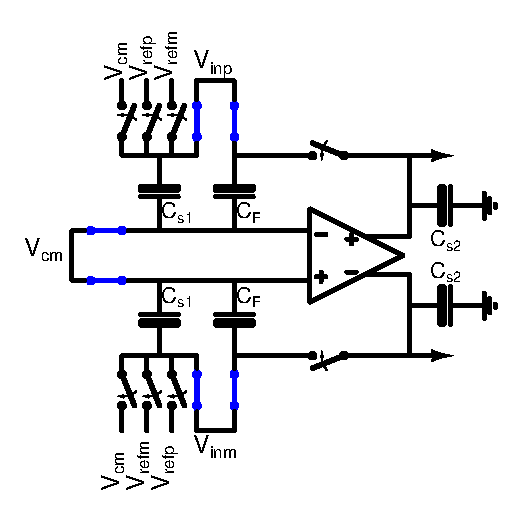
\includegraphics[width=\textwidth]{Chapter4/Figs/algorithmic-mdac-p1.ps}
		\subcaption{first clock cyle:sampling}
		\label{fig:algo-p1}
	\end{subfigure}
	\begin{subfigure}[b]{0.32\textwidth}
		\centering
		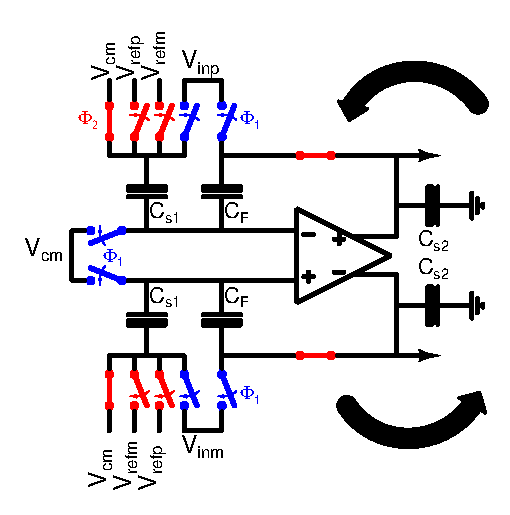
\includegraphics[width=\textwidth]{Chapter4/Figs/algorithmic-mdac-p2.ps}
		\subcaption{even clock cycles}
		\label{fig:algo-p2}
	\end{subfigure}
	\begin{subfigure}[b]{0.32\textwidth}
		\centering
		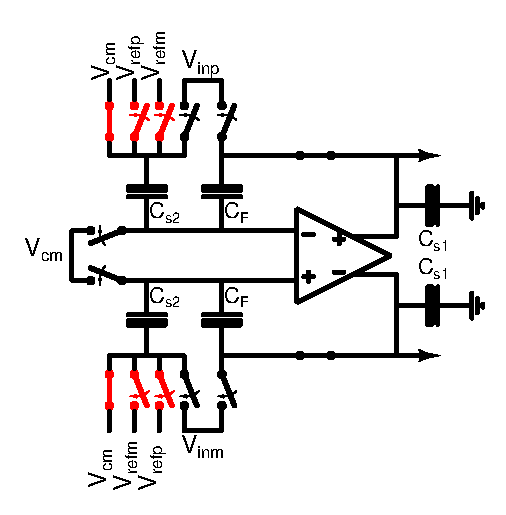
\includegraphics[width=\textwidth]{Chapter4/Figs/algorithmic-mdac-p3.ps}
		\subcaption{odd clock cycles}
		\label{fig:algo-p3}
	\end{subfigure}
	\caption{Proposed sequencing to relax Flip-Around MDAC timing constraints}
	\label{fig:algo-seq-proposed}
\end{figure}

During the first clock cycle, the behaviour is almost identical with the FA-MDAC at the exception of a capacitor \(C_{S2}\) connected on the residue and the local ground as depicted by \figurename~\ref{fig:algo-p1}. Meanwhile, the 3-levels quantizer estimates the feedback voltage to apply such that the residue is constrained in the desired output range. In a second clock cycle, \figurename~\ref{fig:algo-p2}, \(C_F\) is in feedback mode while a feedback is applied to the original sampling capacitor \(C_{S1}\). These two clock cycles is equivalent to the two clock phase of the FA-MDAC first clock cycle. \(C_{S2}\) connected on the residue is accurately sampling the next input. The residue at the end of the second clock cycle is given by equation~(\ref{eqn:algo_res_p2}).

\begin{align}
 \Delta Q_{\Phi_{1 \rightarrow 2}} &= C_{S1} \left[\left(V_{\rm ref}[2]-V[2]^- \right) - \left(V_{\rm inp}-V[1]^- \right) \right] + C_{F} \left[\left(V_{\rm op}[2]-V[2]^- \right) - \left(V_{\rm inp}-V[1]^- \right) \right] \\
 &+ C_{S2} \left[V_{\rm op}[2]-V_{\rm op}[1] \right] \nonumber \\
 V_{\rm op}[2] &= \frac{C_F + C_{S1}}{C_{S2}+C_F\left(1+\frac{C_F+C_{S1}}{AC_F} \right)} \left(V_{\rm inp}-V_{\rm cm} \right) - \frac{C_{S1}}{C_{S2}+C_F\left(1+\frac{C_F+C_{S1}}{AC_F} \right)} V_{\rm ref}[2] + \frac{C_{S2}}{C_{S2}+C_F\left(1+\frac{C_F+C_{S1}}{AC_F} \right)} V_{\rm cm}
 \label{eqn:algo_res_p2}
\end{align}

This implementation follows the same equation as the conventional FA-MDAC\@. A global factor scale down the residue by two in comparison. As the residue is scaled down, large steps occurs less often such that OTA constraints on the gain is relieved.

Then, the sampling capacitors are swapped without breaking the feedback loop made by \(C_F\) as in \figurename~\ref{fig:algo-p3}. Again, the 3-levels quantizer estimates the feedback voltage to constraint the residue within the desired output range. In the next clock cycle, sampling capacitors are swapped and a new feedback voltage estimation is performed by the 3-levels quantizer. This process repeats over and over, \figurename~\ref{fig:algo-seq-proposed},till the last clock cycle in which the 3-levels quantizer outputs the two first bits of the following stage.
\rm 
\begin{align}
	\Delta Q_{\Phi_{2 \rightarrow 3}} &= C_{S1} \left[\left(V_{\rm op}[3] \right) - \left(V_{\rm ref}[2]-V[2]^- \right) \right] + C_{F} \left[\left(V_{\rm op}[3]-V[3]^- \right) - \left(V_{\rm op}[2]-V[2]^- \right) \right] \\
	&+ C_{S2} \left[\left(V_{\rm ref}[3] - V[3]^- \right) - V_{\rm op}[2] \right] \nonumber \\
	V_{\rm op}[3] &= \frac{C_{S2}+C_F\left(1+\frac{C_F+C_{S1}}{AC_F} \right)}{C_{S1}+C_F\left(1+\frac{C_F+C_{S2}}{AC_F} \right)} \left(V_{\rm inp}-V_{\rm cm} \right) - \frac{C_{S2}}{C_{S1}+C_F\left(1+\frac{C_F+C_{S2}}{AC_F} \right)} V_{\rm ref}[3] + \frac{C_{S2}}{C_{S1}+C_F\left(1+\frac{C_F+C_{S2}}{AC_F} \right)} V_{\rm cm}
	\label{eqn:algo_res_p3}
   \end{align}

This operation sequence, compared to the conventional sequence, looses a clock cycle: the two phase operation of the first clock cycle spread onto the two first clock cycles. Nevertheless, the timing constraints on the OTA and the comparator stress are relieved. The comparators have \(T_{clk}-T_{settling}-T_{setup}-T_{logic}\) to make a decision, while the accuracy of the residue voltage can be reached for a longer settling time \(T_{settling}\). Moreover, much OTA architectures have a minimal load criterion to ensure a minimum phase margin and an extra load that \(C_{S2}\) represents enhance the settling of marginally stable OTA\@.

\begin{figure}[htp]
	\centering
	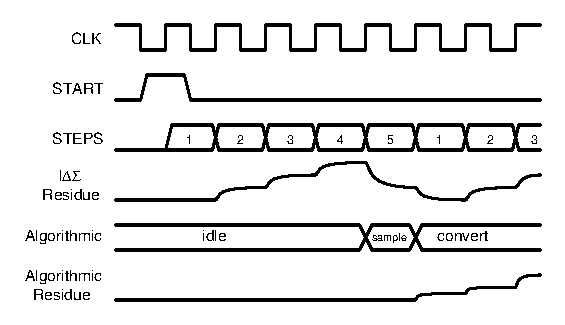
\includegraphics[width=0.75\textwidth]{Chapter4/Figs/isd-algo-residue-sampling.ps}
	\caption{Sampling instant of the I\(\Delta \Sigma \) residue}
	\label{fig:digital-sampling}
\end{figure}

With the proposed sequencing, the sampling instant is twice the time span of the conventional one. As a result, \figurename~\ref{fig:digital-sampling} represents the initialization of the ADC and when the residue of the first stage is sampled by this algorithmic sub-ADC\@. As the first stage reset the integrator during the first clock cycle, the algorithmic shall sample during whole the fifth clock cycle rather than half of this clock period. Therefore, the speed constraints on the first stage is relaxed.

	\subsubsection{1.5-bit DAC}             % section 5.2.3
In the same fashion done for the first-stage Incremental-\(\Delta\Sigma \), the 3-levels quantizer is implemented by the comparison of passive differential voltage summation. With the specificities of this sub-ADC, the 3-levels quantizer shall be able to change its threshold voltages on the last clock cycle to generate the two-firsts bits of the SAR\@. The design procedures addressed in Section~\ref{sec:isd-3-levels-quantizer}, this section will discuss the reference voltage change and its implication on the residue. For the conventional algorithmic sizing (a = 2, b= 1), it is noteworthy that there is no reference voltage change mandatory.

\begin{figure}[htp]
	\centering
	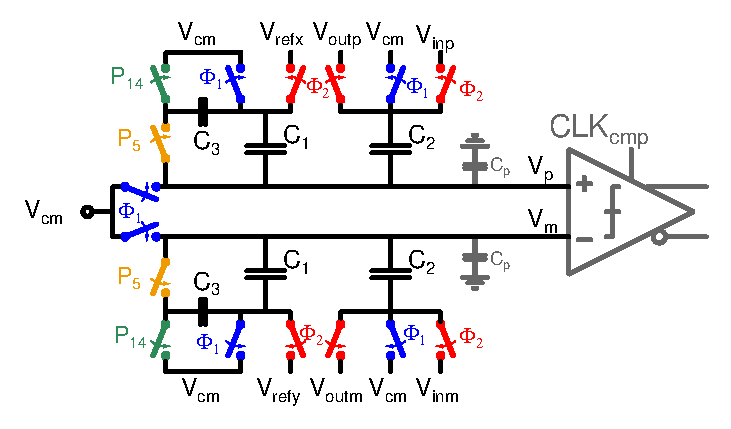
\includegraphics[width=0.75\textwidth]{Chapter4/Figs/algo-passive-adder-comp.ps}
	\caption{Threshold change in the conversion process}
	\label{fig:thresholds-generator}
\end{figure}

\figurename~\ref{fig:thresholds-generator} depicts one possibility to achieve the threshold change. \(C_1\) and \(C_2\) operates as demonstrated in the Section~\ref{sec:isd-3-levels-quantizer}. At the last clock cycle denoted \(P_5\) in the figure, the capacitor \(C_3\) connects to the input voltages of the comparator. This way, the ratio of \(V_{\rm refx}\) is defined by \(\frac{C_1+C_3}{C_2}\) rather than \(\frac{C_1}{C_2}\).

This solution does not let any floating nodes while the behaviour is fully defined by the procedure presented for the first stage. In order to size the capacitor, we consider a unit capacitance \(C_0 = 12 fF\) such that \(C_1 = 3 C_0\), \(C_2 = 10 C_0\), and \(C_3 = 2 C_0\).

The impact on the residue is thus coming from the mismatch. The commit error increases the residue range by an amount \(\varepsilon_{\rm res}\) given by equation~(\ref{eqn:error-residue-algo-quantizer}) for an assumed ideal gain of 2. This expression is valid from the first to the penultimate clock cycle where \(V_{\rm d_i}\) is the differential voltage applied to \(C_i\) capacitors.

\begin{equation}
	\label{eqn:error-residue-algo-quantizer}
	\varepsilon_{\rm res} = 2\left(\frac{\Delta C_1 + \Delta C_2}{C_1+C_2+C_p}\left(\sum_{i=1}^{2}{\Delta C_i V_{\rm d_i}}\right)
	- 2\left(1-\frac{\Delta C_1 + \Delta C_2}{C_1+C_2+C_p}\right)\left(\sum_{i=1}^{2}{\Delta C_i V_{\rm cm_i}}\right)\right)
\end{equation}

In the same manner, the error committed on the last clock cycle engender a mismatch on the two first bits of the SAR\@. This error is likely given by equation~(\ref{eqn:error-residue-algo-quantizer-last}).
\begin{equation}
	\label{eqn:error-residue-algo-quantizer-last}
	\varepsilon_{\rm res} = 2\left(\frac{\Delta C_1 + \Delta C_2 + \Delta C_3}{C_1+C_2+C_3+C_p}\left(\sum_{i=1}^{3}{\Delta C_i V_{\rm d_i}}\right)
	- 2\left(1-\frac{\Delta C_1 + \Delta C_2 + \Delta C_3}{C_1+C_2+C_3+C_p}\right)\left(\sum_{i=1}^{3}{\Delta C_i V_{\rm cm_i}}\right)\right)
\end{equation}

	\subsubsection{Digital Circuit}         % section 5.2.4	
\textbf{\textcolor{black}{define what is reused in the digital:}}
To drive the analog core, the digital circuit also needs a clock generator, a sequencer, and driver interfaces. The sequencer and the clock generator present inside the digital circuit of the first stage are re-used while the driver interfaces are instantiated again for the switches command signal of this stage. The new sequencing no more based on clock phase for the MDAC, the clock phase generated only serve the purpose of the 3-levels quantizer.

\textbf{\textcolor{black}{the problematic of non overlapping without using clock phases:}}
As switches in the MDAC connect several analog reference voltages on the same capacitor plates, non overlaps shall be respected to prevent the short circuit of them. In order to improve both the sustainability and the yield, the non-overlap time in the digital circuit shall be fully ``synthetizable''. Then, non overlapping time being part of the digital static timing analysis, such cells ensure the operation with an increased reliability on the sub-ADC\@.

\textbf{\textcolor{black}{solution 1:}}
A first possible realization could be the one depicted by \figurename~\ref{fig:solution-1}. This solution can be implemented with standard digital tools with a pulse generation based on a clock and a delayed one. Unfortunately, this circuit suffers from possible glitches due to the multiplex of DFF outputs and clocks are used in a data path.

A Double-Edge circuit is able to implement the functionality desired as one clock sets the value to block analog switches till a delayed clock sample the signal to activate the analog switches. A usual realization is built around two pulse generation to trigger a latch at two distinct instant~\cite{Afghahi1996, Cheng2003dig, Murotiya2013, Bonetti2015}. Pulses generation is considered as an analog circuit for which digital tools cope with badly.

\begin{figure}[htp]
	\centering
	\begin{subfigure}[b]{0.48\textwidth}
		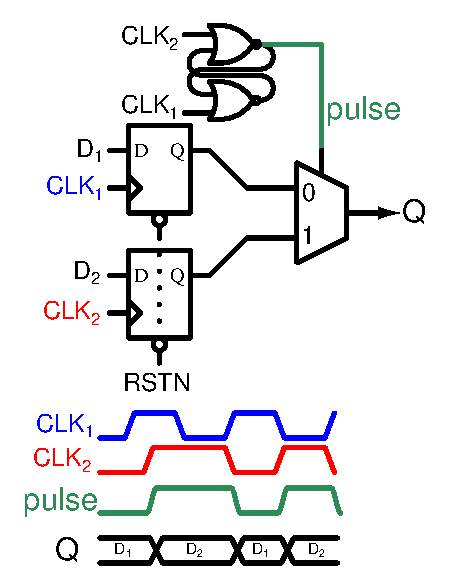
\includegraphics[width=\textwidth]{Chapter4/Figs/det-dff-solution1.ps}
		\subcaption{multiplexed DFF}
		\label{fig:solution-1}
	\end{subfigure}
	\begin{subfigure}[b]{0.48\textwidth}
		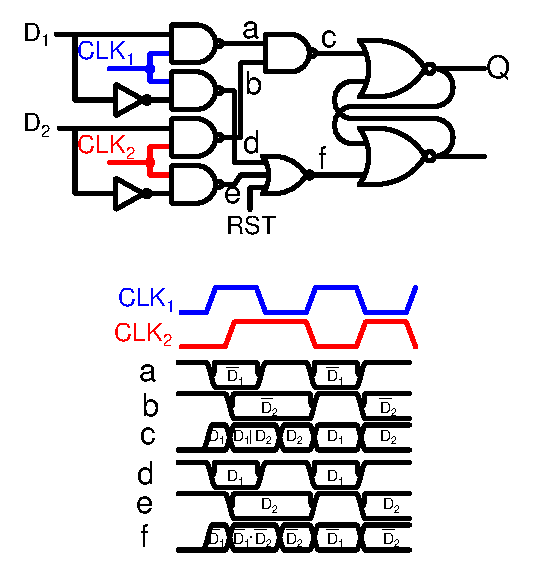
\includegraphics[width=\textwidth]{Chapter4/Figs/det-dff-solution2.ps}
		\subcaption{double edge latch}
		\label{fig:solution-2}
	\end{subfigure}
	\caption{Possible realization of the dual-edge trigger D-Flip-Flop}
	\label{fig:digital-non-overlap}
\end{figure}

\textbf{\textcolor{black}{solution 2:}}
In response, \figurename~\ref{fig:solution-2} represents an alternative based on combinatorial logic. This clocked nor rs-latch with a reset generates a new dual-edge DFF with a distinct data path from the clock path. From a timing point of view, the non overlap between \(CLK_1\) and \(CLK_2\) shall be ideally ensured. Otherwise a glitch can occur for arbitrary \(D_1\) and \(D_2\). In case of \(D_1 = 0\), the overlapping of \(CLK_1\) and \(CLK_2\) is no more a concern. For timing constraints, the cell is sensitive to the placement.

\textbf{\textcolor{black}{solution 3 (the one kept):}}
Proposed by Ralf Hildebrandt, such a block can be described with only two DFFs without mixing of the clock and data path and no possibility for glitches. This proposition is represented in \figurename~\ref{fig:digital-non-overlap} after a change of \(CLK_2\) as a delayed \(CLK_1\). Therefore, there is no hold time issue and the setup time constraint relaxed on the DFF triggered by \(CLK_1\) put under pressure the DFF triggered by the delayed clock. Over temperature the transition time of analog switches increases as the non overlap time defined by the delay between the two clocks does.

\begin{figure}[htp]
	\centering
	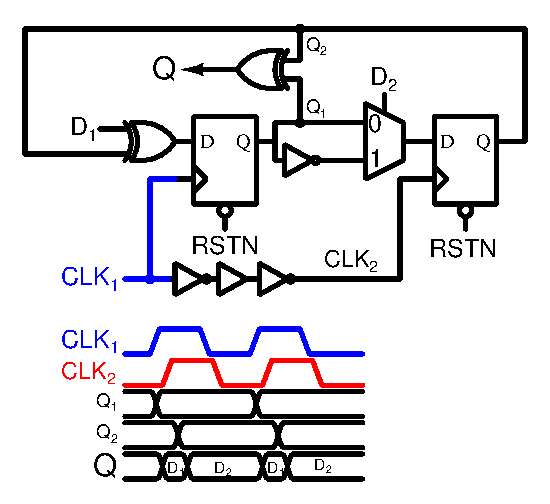
\includegraphics[width=0.6\textwidth]{Chapter4/Figs/det-dff-hildebrandt.ps}
	\caption{Synthetizable non-overlap circuit without failure in the static timing analysis}
	\label{fig:digital-non-overlap}
\end{figure}

Then, the latter is followed by digital driver presented in Section~\ref{sec:dig-driver} to prevent ambiguity in the sampled value when the settling time is limited and the non-overlapping time is short.

For switches in the 3-levels quantizer, two non overlapping clock phases are required. The already mentioned clock phase generator circuit of the first stage fits this purpose. A particular caution is paid at the clock phase connection such that the sampling occurs when the settling is almost performed around the instant of the falling edge of the main clock. As the delay between our pseudo dual edge trigger DFF (pseudo-DET-DFF) reduces the settling time, the clock tree skews gain much importance. For accurate results, the clock of the clock phase generator shall be late in comparison of the clock provided to the pseudo-DET-DFFs.

The algorithmic ADC is known to be sensitive to analogue defects. At a system-level, the architecture and the conversion sequencing have been thought to reduce the error on the settling of the residue. From the equation of the error in the MDAC, we consider the introduction of an interstage gain $g$, and a tunable feedback gain $f$. The two candidate pairs of values exhibiting a reduce error are the conventional design ($g$=1, $f$=1), and ($g$=1, $f$=1.2).
To facilitate the digital implementation of non-overlapping command signal without clock phase, the digital interface has been investigated. The selected circuit allows the introduction of a scan chain, and simplifies the layout phase without introducing failure in the timing analysis.
\clearpage
\subsection{SAR}                            % section 5.3
The SAR architecture benefits from using only one comparator to reduce the occupied area. With recent progress, the SAR converter outperformed power consumption, its area occupancy has tremendously shrunk, and the speed has been soaring. Made of a capacitive DAC, a comparator, and a digital control circuit, the primary source of power dissipation are the digital control circuit and capacitive reference DAC network, while the source of large area occupancy is the capacitive DAC\@.

Since the two first bits of the SAR are given by the previous stage, one clock cycle will be used for pre-charging capacitors, and remaining clock cycles before the next sample extract more information. In consequence with 5 clock cycles, the SAR provides 6 bits. An adaptation of the DAC is necessary.

In addition to the specification, an extra mode exists to increase the resolution of the ADC by sacrificing the sampling rate. This extra mode performs a conversion over 6 clock cycles instead of 5. While this does not impact the structure of the analog in the two preceding stages, several modifications are required in this sub-ADC\@. Therefore, we discuss in this section of the relevant modification in the capacitive reference DAC network and in the digital circuit.

	\subsubsection{Capacitive DAC Array}    % section 5.3.1
	\label{sec:capacitive-dac-sar-design}
To address both the area occupancy and further reduce the energy consumption, the DAC architecture can be optimized by decreasing the capacitance as discussed in section~\ref{sec:sar-adc}. For thermal noise reason of switches, the split-capacitor structure is preferred over split-junction.

\begin{figure}[htp]
	\centering
	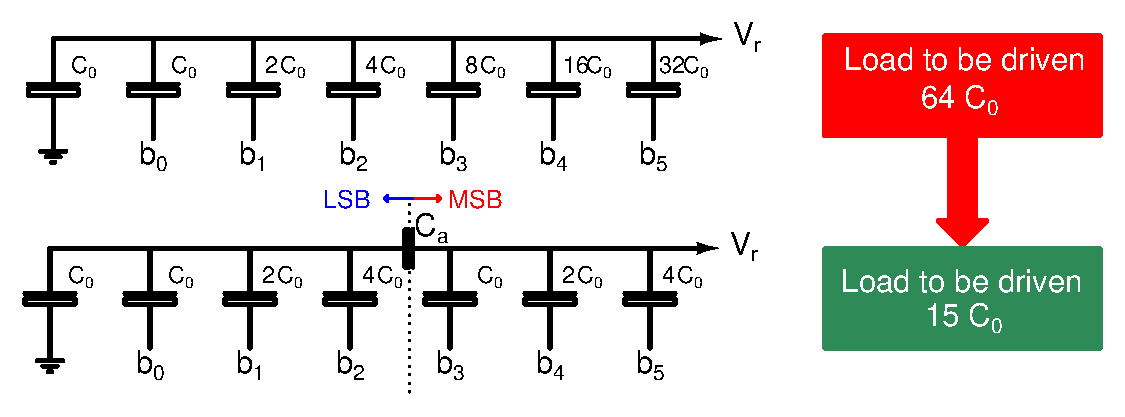
\includegraphics[width=\textwidth]{Chapter4/Figs/sar-dac-normal-split-cap.ps}
	\caption{Load reduction for both the OTA of the Algorithmic and the voltage references buffers}
	\label{fig:sar-dac-normal-split-cap}
\end{figure}
\textbf{\textcolor{black}{position of the attenuation capacitor to minimize the load:}}
In \figurename~\ref{fig:sar-dac-normal-split-cap}, the position of the attenuation capacitance \(C_a\) can be placed between either group of two consecutive capacitors of the DAC, which create a group of \textcolor{red}{MSB} capacitors and a group of \textcolor{blue}{LSB} capacitors. The attenuation capacitor is at the position which minimize the load seen by voltage references and the previous stage OTA\@.

\textbf{\textcolor{black}{parasitic insensitive:}}
Switches connecting either voltage of the following set \(\left\{ V_{\rm in}, V_{\rm refp}, V_{\rm refm} \right\} \) are on the bottom plate (side opposite to the comparator input). It makes the DAC inherently insensitive to switches' parasitic capacitance and still keep the criterion on accurate reference voltages \(\varepsilon_{\rm references} < 1 LSB\).

\textbf{\textcolor{black}{voltages generated and scale:}}
By application of superposition, the output voltage \(V_r\) is given by equation~(\ref{eqn:output_voltage_dac_sar}) where \(C_i\) the capacitor connected to the voltage \(b_i V_{\rm ref}\) of the aforementioned figure. A consequence of the attenuation capacitor is the difficult implementation to have both a binary scale and \(C_a\) a multiple integer of the unit capacitance \(C_0\).

\begin{align}
	\label{eqn:output_voltage_dac_sar}
	V_r &= \frac{\left(C_a + \sum_{i \in LSB}{C_i}\right)}{\left(C_a + \sum_{i \in LSB}{C_i}\right)\left(C_a + \sum_{i \in MSB}{C_i}\right)-C_a^2} \sum_{i \in MSB}{C_i b_i} V_{\rm ref} \nonumber \\
	&+ \frac{C_a}{\left(C_a + \sum_{i \in LSB}{C_i}\right)\left(C_a + \sum_{i \in MSB}{C_i}\right)-C_a^2} \sum_{i \in LSB}{C_i b_i} V_{\rm ref}
\end{align}

In the case of ideal value of the attenuation capacitor $C_a = 8/7$ for a configuration as represented in \figurename~\ref{fig:sar-dac-normal-split-cap}, the voltage contribution of each capacitor driven by $b_5$ to $b_0$ is respectively \{0.5, 0.25, 0.125, 0.0625, 0.03125, 0.015625\}.

\textbf{\textcolor{black}{second stage decision error:}}
The previous stage generating the two first bits of the SAR, an erroneous decision of the algorithmic impacts the overall decisions of the SAR and cannot be fully corrected. Without any redundancy as represented in \figurename~\ref{fig:std-scale}, an error in the decision made by comparators providing a 01 instead of a 10 corresponds a final error of 1 LSB\@. The redundancy could be introduced by decreasing the two first bits’ weight \(A_{MSB}\) and \(A_{MSB-1}\): a weight distribution of \(A_i\)'s as 3-1.5-1-4-2-1-1 rather than 4-2-1-4-2-1-1 times the unit capacitor. In fact, keeping \(A_i\) as an integer multiple of the unit capacitor, the version 6-3-2-4-2-1-1 is implemented with an ideal attenuation capacitor of \(8/3\). As depicted by \figurename~\ref{fig:altered-scale-1}, the resulting error is less than 1 LSB\@. The counterpart is a bigger LSB, which is representative of a trade off between robustness and resolution. 

\begin{figure}[htp]
	\centering
	\begin{subfigure}[b]{0.48\textwidth}
		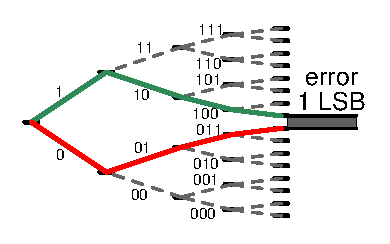
\includegraphics[width=\textwidth]{Chapter4/Figs/sar-binary-scale.ps}
		\subcaption{binary scale}
		\label{fig:std-scale}
	\end{subfigure}
	\begin{subfigure}[b]{0.48\textwidth}
		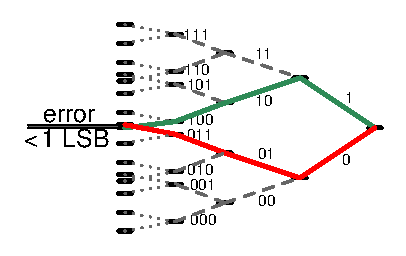
\includegraphics[width=\textwidth]{Chapter4/Figs/sar-non-binary-scale.ps}
		\subcaption{non-binary scale proposed}
		\label{fig:altered-scale-1}
	\end{subfigure}
	\caption{Alteration of the search scale to provide robustness with redundancy}
	\label{fig:sar-redundancy}
\end{figure}

\textbf{\textcolor{black}{attenuation capacitor rounding for redundancy:}}
The attenuation capacitor scaling down the \(A_i\)'s in the LSB part can be an alternative to introduce redundancy. As the ideal attenuation capacitor is most of the time not an integer multiple of the unit capacitor, rounding to the superior integer could be sufficient.

For instance, let us consider two ``capacitors'' in series of which their equivalent capacitance is the weight the smallest capacitor within the MSB group in \figurename~\ref{fig:sar-dac-normal-split-cap}. The size of the attenuation capacitor to ensure ideal scale is given by \(\frac{1}{C_{eq}} = \frac{1}{C_1}+\frac{1}{C_2}\). Similarly, in the case of a split-dac the attenuation capacitor is given by equation~(\ref{eqn:attenuation-cap-size}).

\begin{equation}
\label{eqn:attenuation-cap-size}
\frac{1}{C_{eq}} = \frac{1}{C_a}+\frac{1}{\sum_{i \in LSB}{C_i}}
\end{equation}

For a capacitance \(C_{eq} = 2 \) and \(C_2 = 8\), the expected value of \(C_1\) to ensure the equality is \(8/3 \approx 2.667 \). Rounding the value of \(C_1\) to 3, change the equivalent capacitance to \(24/11 \approx 2.18 \) while a ceiling of \(C_1\) to 2, results into an equivalent capacitance of \(8/5 = 1.6 \). Therefore, rounding the attenuation capacitor gives more weight to the LSB group to be able to alleviate errors of the previous stage. This solution also results into a resolution/robustness trade-off with an easier realization since each capacitance is made of an integer multiple of the unit capacitor. The finale capacitor distribution is thus 6-3-2---4-2-1-1 with an attenuation capacitor of 3 unit capacitor. The reference voltages generated are \{0.5, 0.25, 0.167, 0.091, 0.045, 0.023, 0.011\}.

\textbf{\textcolor{black}{unit capacitor sizing procedure:}}
Based on the procedure formulated in~\cite{Yue2013}, we estimate the noise contribution and the mismatch impact on the resolution of the DAC with respect to the unit capacitor size. We consider that the maximum tolerable error for an N-bit DAC is $\pm 1/2$ LSB which equals $V_{\rm ref}/2^{N+1}$. We suppose that mismatch variation and noise contribution of each capacitor are uncorrelated such that the standard deviation of the error is given by $\sigma^2 = \sigma_{\rm mismatch}^2 + \sigma_{\rm noise}^2$, and we shall constrain the error to within $\pm 1/2$ LSB.

\textbf{\textcolor{black}{matching error contribution:}}
For the expectation of the matching to be relevant, the assumption is a common-centroid layout for the implementation of the DAC to get rid of all gradient related source of mismatch (temperature, mechanical stress, \ldots) to only keep the manufacturing variations. Capacitors split into multiple of unit capacitors with a normal distribution of the unit capacitance $\frac{\Delta C}{C} \approx N(0, \sigma_0^2)$, the mismatch of a single capacitor \(C_i = A_iC_0\) is given by $\frac{\Delta C_i}{C_i} \approx N(0, A_i\sigma_0^2)$ if each unit capacitor variation is independent from the other.

We thus set a limit for the mismatch by the equation~(\ref{eqn:dac-mismatch-error-sizing}) where $N_\sigma$ is the number of standard deviations we consider for the confidence interval, and a LSB error contribution as the maximum error defined in~\cite{Yue2013} weighted by the $C_a/(C_a+\sum_{i \in LSB} C_i)$.

\begin{eqnarray}
 \label{eqn:dac-mismatch-error-sizing}
 \frac{V_{\rm ref}}{2^{N+1}} &\gtq \frac{N_\sigma \sigma_0 V_{\rm ref}}{\sum_{i \in LSB} A_i - N_\sigma \sigma_0 \sqrt{\sum_{i \in LSB} A_i}} \sum_{i \in LSB} \sqrt{A_i} \times \frac{A_a \left(1-N_\sigma \sigma_0 \right)}{\left(A_a + \sum_{i \in LSB} A_i\right) \left(1-N_\sigma \sigma_0 \right)} \nonumber \\
 &+ \frac{N_\sigma \sigma_0 V_{\rm ref}}{\sum_{i \in MSB} A_i - N_\sigma \sigma_0 \sqrt{\sum_{i \in MSB} A_i}} \sum_{i \in MSB} \sqrt{A_i}
\end{eqnarray}

\textbf{\textcolor{black}{noise estimation:}}
Let's now consider the noise introduced by switches on the DAC\@. Assuming switches as a resistance, the voltage standard deviation of the thermal noise \(\Delta V_i\) on a capacitance \(C_i = A_iC_0\) is given by equation~(\ref{eqn:thermal-noise-mult-of-unit-cap}).

\begin{equation}
	\label{eqn:thermal-noise-mult-of-unit-cap}
	\Delta V_i = \sqrt{\frac{k_BT}{A_iC_0}}
\end{equation}

From the equation developed, the output noise on the input of the comparator is defined by the equation~(\ref{eqn:output_noise})

\begin{equation}
	\label{eqn:output_noise}
	\Delta V_r_{\rm noise} = \frac{\left(\frac{C_a}{C_0} + \sum_{i \in LSB}{A_i}\right)\left( \sum_{i \in MSB}{\sqrt{\frac{k_BT}{A_i}}} \right) + \frac{C_a}{C_0} \left(\sum_{i \in LSB}{\sqrt{\frac{k_BT}{A_i}}} \right)}{\left(\frac{C_a}{C_0} + \sum_{i \in LSB}{A_i}\right)\left(\frac{C_a}{C_0} + \sum_{i \in MSB}{A_i}\right)-{\left(\frac{C_a}{C_0}\right)}^2} \frac{1}{\sqrt{C_0}}
\end{equation}

\textbf{\textcolor{black}{unit capacitor size:}}
From thence, and the variation $\sigma_0$ known as a function of $C_0$, the value of the unit capacitance required is given by a Newton-Raphson algorithm. The unit capacitor needed to cope with a $N_\sigma = 6$ is about 48 fF. In comparison a classical DAC would have required a unit capacitance of 42 fF for the same error budget. For the OTA of the second stage, the load to be driven is thus 950 fF saving 1.7 pF. The noise on the voltage to be compared $V_r$ is 847 \(\mu V_{\rm rms} \) at 475\(\degree \)K.

\textbf{\textcolor{black}{modification for a 6 clock cycle operation:}}
\begin{figure}[htp]
	\centering
	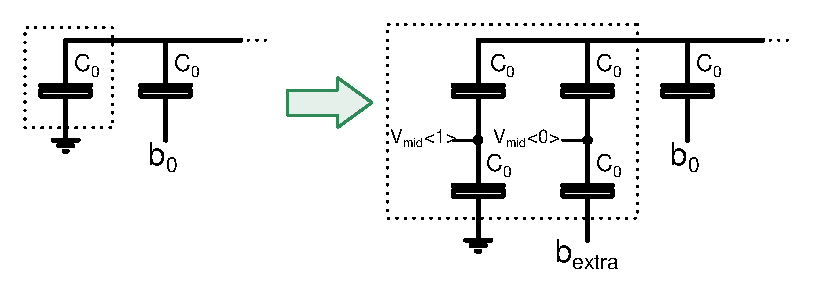
\includegraphics[width=0.8\textwidth]{Chapter4/Figs/sar-extra-clock-cycle.ps}
	\caption{DAC modification to perform conversion with an extra clock cycle}
	\label{fig:sar-dac-extra}
\end{figure}
To allow an operation over 6 clock cycles, the DAC shall be modified in consequence. Usual configuration would implement an extra MSB capacitor doubling the area. Here, the modification consists in splitting the extra unit capacitor not driven into two half the capacitance in parallel. To keep the mismatch low, half the unit capacitance is performed by connecting in series two unit capacitors as represented in \figurename~\ref{fig:sar-dac-extra}.


In a normal 5 clock operation, \(b_{extra}\) is the same potential as the one at its left, such that the block of 4 is equivalent to a unit capacitance \(C_0 \).

Since this modification adds two floating points, voltages \(V_{mid}<1:0> \)are defined when the DAC sample the input voltages. While sampling, in a charge redistribution mode operation, the input voltage is sampled on one end of capacitors. On the other end, capacitors are connected to a virtual ground such as the common mode voltage in a differential circuit. In a differential circuit as ours, \(V_{mid}<1:0> = V_{cm}\) during the sampling. Then, they are disconnected to let the chosen switching scheme drives voltage applied on a half capacitance. The resulting DAC is presented in \figurename~\ref{fig:sar-dac-full}.

\begin{figure}[htp]
	\centering
	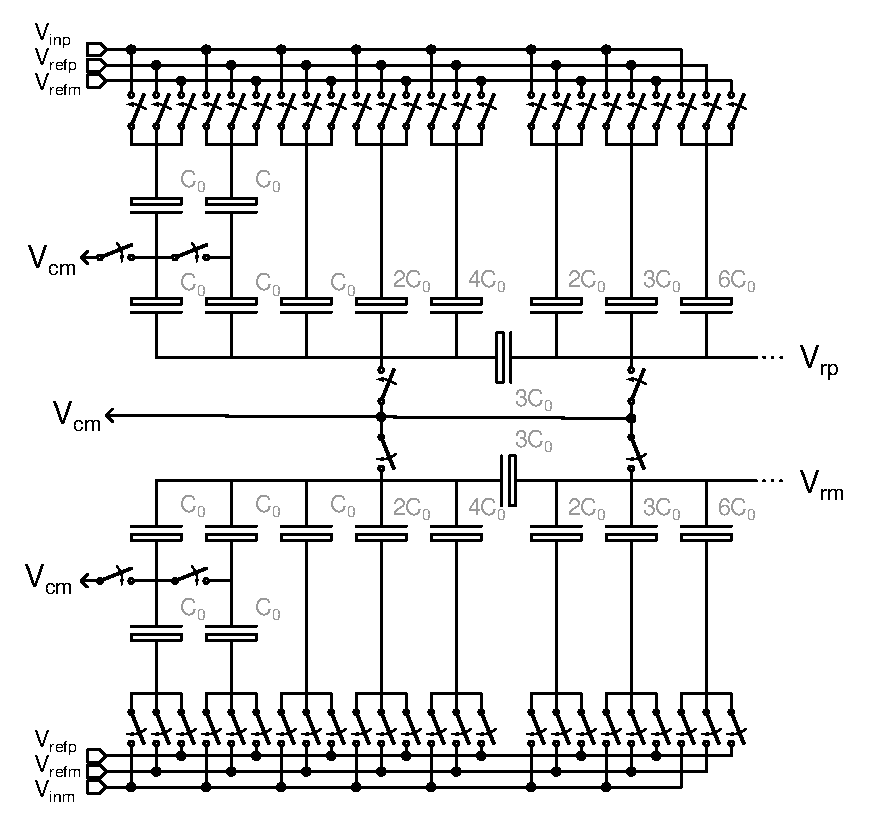
\includegraphics[width=0.75\textwidth]{Chapter4/Figs/sar-dac-full.ps}
	\caption{Final DAC schematic for the SAR}
	\label{fig:sar-dac-full}
\end{figure}

	\subsubsection{Switching Scheme}        % section 5.3.2
Based on the discussion in Section~\ref{sec:sar-switching}, the conventional charge-redistribution method is not power effective~\cite{Ginsburg2005}. A monotonic switching can divide by almost two the switching loss as the MSB capacitor is no more necessary. However, the common mode voltage undergoes decision dependant large variations. Represented in \figurename~\ref{fig:sar-vcm-change-monotonic} for the sake of comprehension, a monotonic based switching keeps the \(V_{\rm cm} \) within the input range. For each decision made, as only one voltage is altered at a time, the common mode voltage  inevitably fluctuates from one clock period to another. Let's suppose the final output code is full of ones, the common mode voltage will be ever increasing to reach the maximum input voltages. While for a final output code full of zeros, the common mode voltage will be ever decreasing to reach the minimum input voltages. This is a high-demanding input range on the comparator performance for a switching power consumption relaxed. At least with a $V_{\rm cm}$-monotonic once the decision is made, the decision is applied on both sides by the application of complementary voltages to keep the common mode voltage around half $V_{\rm DD}$.

\begin{figure}[htp]
	\centering
	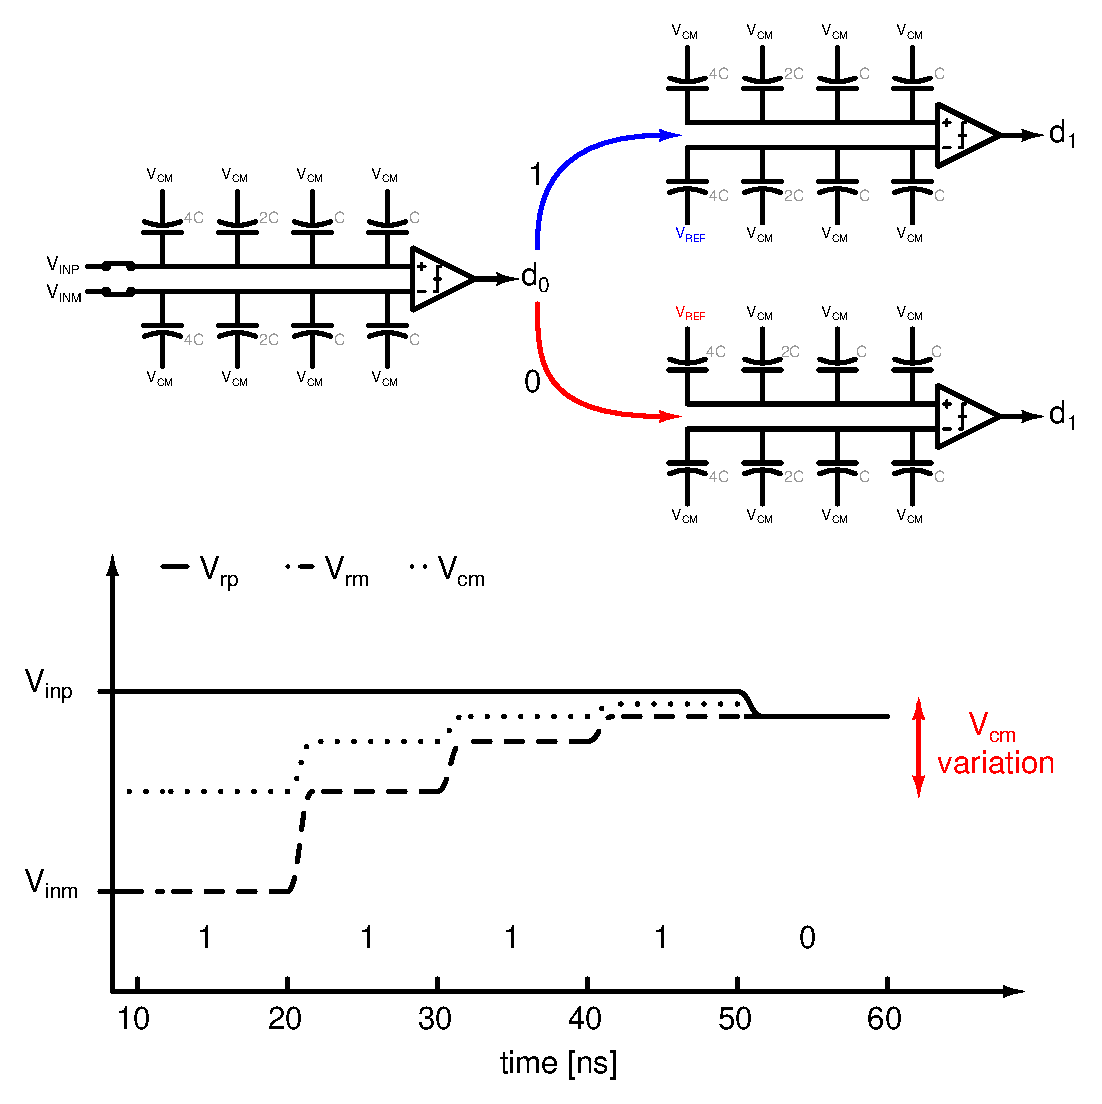
\includegraphics[width=0.75\textwidth]{Chapter4/Figs/sar/sar_vcm_monotonic-vcm-change.ps}
	\caption{Change of the common mode voltage in a monotonic based digital scheme}
	\label{fig:sar-vcm-change-monotonic}
\end{figure}

Unfortunately, both monotonic switching methods rely on a top sampling technique. To the contrary the bottom plate sampling of the conventional charge-redistribution is related to better linearity and higher resolution: the method reduces the effect of charge injection during switching off and the non-linearity of the junction capacitance of the top plate switch is negligible. As the charge injection of switches is a linear function of the temperature at a rate of \(C_{ox}WL\alpha_{V_{th}}\), the conventional switching scheme has been selected.

	\subsubsection{Digital Circuit}         % section 5.2.3 
As the clock frequency increase, or as the temperature degrades the speed of the analog part, the digital constraints on a SAR become challenging. The timing constraint is defined by the time the DAC requires to settle to the wished accuracy, the delay of the comparator, and the time the logic need to respond.

\textbf{\textcolor{black}{synchronous:}}
In a synchronous SAR, the high demand is assumed on the comparator to latch as fast as necessary to let the digital toggle switches according to the decision made. The clock period is usually defined on the worst speed corner for the lowest power supply voltage and the higher temperature.

\textbf{\textcolor{black}{asynchronous:}}
To the contrary an asynchronous SAR waits for the comparator decision and ``digital'' does not wait for an edge of the clock. For unusually too long decision time, the digital code might be incomplete and results in errors. Forcing the decision in case of metastability did not have the same impact on the digital code representation of the input compared to an erroneous decision. Indeed, the metastability occurs in decisions where the inputs of the comparator are close enough to prevent either the noise or mismatch to set the decision value within the allotted time. A comparator sensing a difference less than an LSB is sufficient.

\textbf{\textcolor{black}{synchronous versus asynchronous:}}
This first modification in the operation increases the allotted time for the comparator to make a decision: the probability of the metastability is highly reduced for the same comparator while the power consumption can be reduced for the same probability of metastable events.

\figurename~\ref{fig:sar-sync-async} compares the synchronous and the pseudo-asynchronous operation which forces the decision in case of metastability. The instants in delimited by blue boxes represents the domain when the decision shall be made to ensure correct operation based on setup and hold violation in the logic. Although, in a synchronous digital scheme the time window is ``constant'', in the proposed version the time window is at least equal or greater. The stringent constraints on the comparator is thus relaxed. 

Assuming the clocked comparator delay follows a small signal model of a cross-coupled latch with regeneration time constant \(\tau_{reg} \), link the differential input voltage \(\Delta V_{\rm in}\) pre-amplified in a linear phase, to the decision time as in~(\ref{eqn:comp-model-delay-basic}).

\begin{equation}
	\label{eqn:comp-model-delay-basic}
\Delta V_{out}(t) = \Delta V_{out}(0) \exp\left(\tau_{reg}\right)
\end{equation}

The probability to generate an erroneous decision depends on the input voltage applied, the temperature, the process and can further generate metastability  within the logic as described in Appendix~\ref{app:comp-metastability}. Considering a synchronous ADC, failures in digital circuit due to metastability is critical and missing a most significant bit should be prevented.

\begin{figure}[htp]
	\centering
	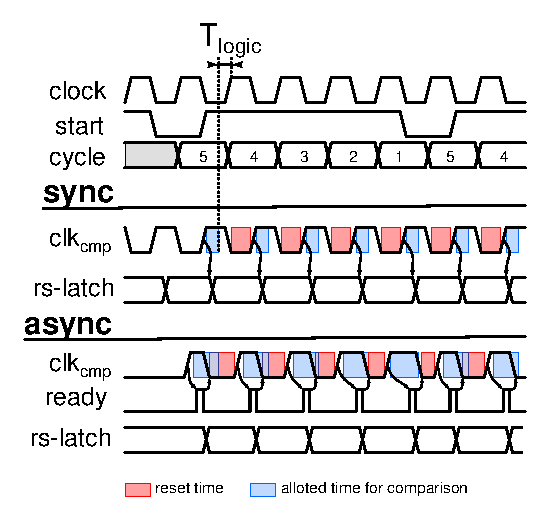
\includegraphics[width=0.75\textwidth]{Chapter4/Figs/sar-comp-constraint.ps}
	\caption{Comparator constraint relaxed by the use of pseudo-synchronous digital scheme}
	\label{fig:sar-sync-async}
\end{figure}

Furthermore, a comparator making a decision quickly also benefits from a long time to reset. Otherwise, a reduce reset time engenders a hysteresis owing to a mismatch in the potential of parasitics. The hysteresis introduced is thence state dependant and vary from one clock cycle to the other. 

% to be changed with the real formula based on the MTTF
In the design of the latch, the delay shall be less than \(T_{clk} -  T_{logic} - T_{settlingDAC}\). Without considering the clock skew the comparator delay can be as large as 7 ns. This value does not consider the clock skew. Nevertheless, to reduce the metastability to a maximum without increased tremendously the power consumption the delay have been fixed to 3 ns at maximum with a standard variation of 500 ps.

In the case of a SAR ADC clocked at 100 MHz with the proposed digital scheme, the probability of a metastable event to occur is estimated to be less than $10^{-18}$ at 175$\degree C$ (Appendix~\ref{app:comp-metastability}): the typical lifetime of an electronic component is not sufficient to be sure to see a metastable event.

\textbf{\textcolor{black}{sequencer:}}
Considering PVT variations and the case of the metastability, an asynchronous digital is implemented. To prevent halt in the conversion, the clock provides a time slot in which a flag is raised at the end to indicate the metastability and force the execution of subsequent cycles as in~\cite{Tung2016}. This ensures at the end of the conversion a digital code of the desired length and easily interfaceable with a synchronous digital.

The sequencer resulting is depicted in \figurename~\ref{fig:sar-async-sequencer} to generate the phase in one hot encoding. In front of the first DFF, the logic allows continuous conversion for a START signal hold to zero. Therefore, the digital sequencer can be halted and resume the conversion process without a reset.

\begin{figure}[htp]
	\centering
	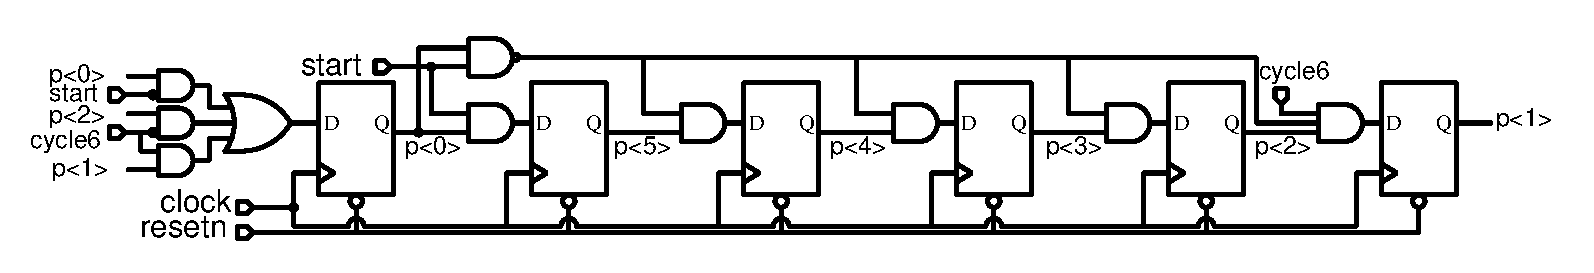
\includegraphics[width=\textwidth]{Chapter4/Figs/sar-sequencer.ps}
	\caption{Synchronous sequencer to force decision in case of metastability}
	\label{fig:sar-async-sequencer}
\end{figure}

\textbf{\textcolor{black}{comparator clock generation:}}
To relax constraints on the comparator, asynchronism is introduced in the clock generation as well as in switches command. Inside the clock generation circuit represented in \figurename~\ref{fig:sar-clock-gen}, the possibility between a synchronous and a generated clock is allowed with the clock mixer. For the sake of implementation, the delay of the inverter at the data input of the DFF shall be long enough to prevent a hold violation.

In a fully synchronous design, the comparator makes decision on falling edge of the primary clock, whereas in a pseudo-synchronous design the reset of comparators is triggered \(T_{nor} + T_{dff} + \(T_{mux} \) after a decision have been made. This allows a nor-rs-latch to store the result of comparison for the full clock cycle.

\begin{figure}[htp]
	\centering
	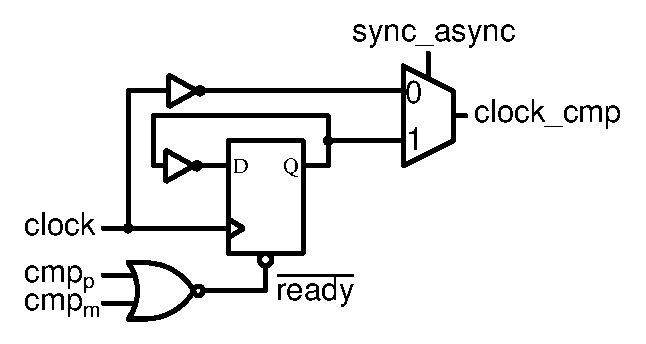
\includegraphics[width=0.5\textwidth]{Chapter4/Figs/sar-clock-generator.ps}
	\caption{Comparator clock generation to select a pseudo-synchronous operation or fully synchronous behaviour}
	\label{fig:sar-clock-gen}
\end{figure}

For cmos cross-coupled inverter based lathes, the reset phase can consume as much energy as during the state of a decision have been made. The modification does not improve the power consumption. Nevertheless the redundancy being an intrinsic property of the DAC, a settling error is corrected by following clock cycles. The redundancy allows to trigger the comparator earlier, while the settling is not complete.

\textbf{\textcolor{black}{switches design:}}
For the selected digital scheme, switches shall connect the input voltages during the sampling clock cycle. Then each capacitor weight is tested from the most significant weight to the least significant one. This is done by connecting \(+V_{\rm ref}\) (\(V_{\rm refp}-V_{\rm refm}\)) on capacitors whose weight is not being under test and to the others \(-V_{\rm ref}\) (\(V_{\rm refm}-V_{\rm refp}\)).

To not introduce settling error the positive reference voltage is connected to capacitors via low-vt pmos transistors, the negative reference voltage by low-vt nmos transistors, and the input via transmission gates whose pmos is 3.5 times bigger than nmos. In addition to that, only one switch is active at a time: the transmission gate only during the sampling clock cycle, and then either the pmos or the nmos.

\begin{figure}[htp]
	\centering
	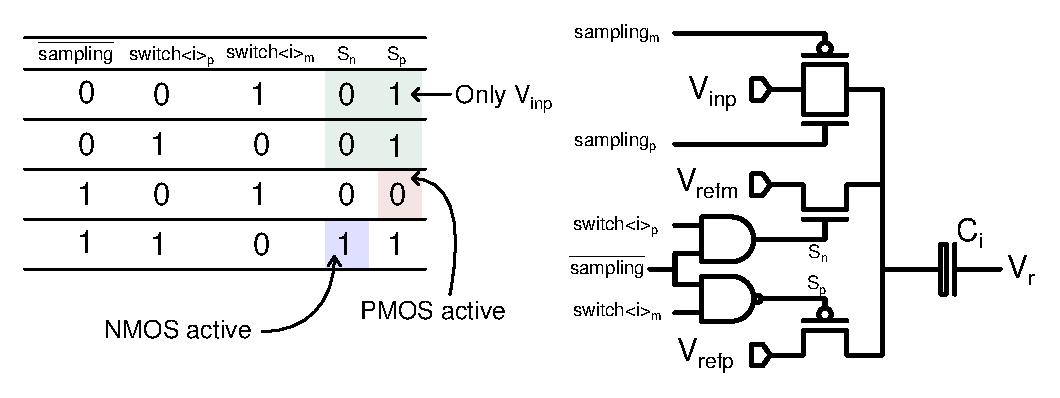
\includegraphics[width=\textwidth]{Chapter4/Figs/sar-switches-command-simp.ps}
	\caption{The switches signal command to connect only one voltage at a time of the connected capacitor}
	\label{fig:switches-command}
\end{figure}

As represented in \figurename~\ref{fig:switches-command}, the 4 wires are present. \(S_n\) and \(S_p\) are generated from a common signal and the complementary of sampling. The truth table on highlights which switch is active to ensure that only one is active.

The common signal is thus a predefined waveform which is reset to one for the sampling clock cycle, set to zero for the clock cycle to test the capacitor connected to the switch, and then set to the result of the comparison made by the comparator. The generation of each signal follows the same pattern depicted by \figurename~\ref{fig:comp-decision-switches}.

% the utmost right sr latch is a nand one, therefore, the S=1 --> Q = 0
\begin{figure}[htp]
	\centering
	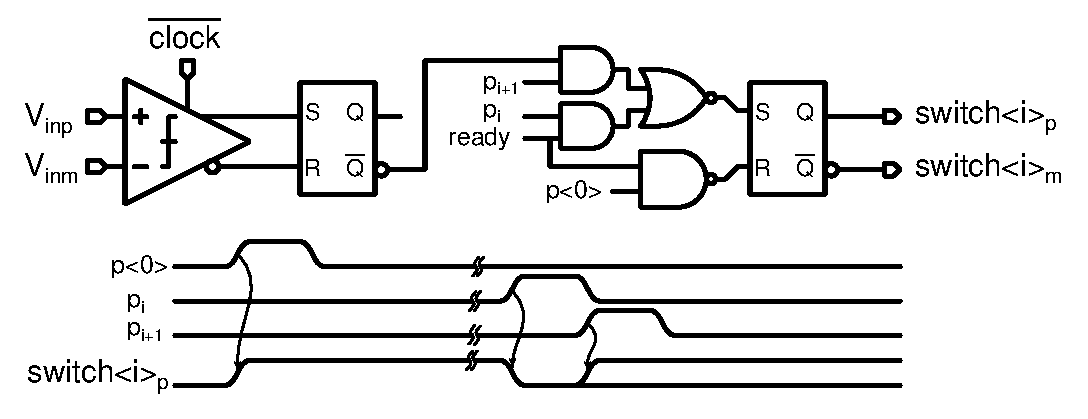
\includegraphics[width=0.78\textwidth]{Chapter4/Figs/comp-decisin-switches.ps}
	\caption{Switches signal command based on the decision of the comparator}
	\label{fig:comp-decision-switches}
\end{figure}

This SAR has the purpose to extract final bits in the conversion for an insignificant fraction of the ADC power consumption. In the analogue domain, the capacitance of the DAC has been reduced by the employ of a split-DAC technique. The energy consumption can be further scaled down by changing the digital switching scheme at a price of a common-mode voltage variation, in turn impacting the comparator.

Considering, the possible error in the decision and variation in the DAC due to manufacturing, a redundancy is introduced. The redundancy is helpful to reach higher sampling rates with a slow comparator. Unfortunately, the redundancy does not reduce the latch metastability and its repercussion on the digital. Henceforth, a pseudo-asynchronous digital gives a margin to reduce the probability of a metastable event.

So far, the design of each stage is independent of each other and assumption on the amplifiers are numerous. Simulations of the ADC thus follow.

% Despite the most sensitive bloc of this stage is the capacitive DAC, there is indubitable specificities worth to mention. This section therefore relates constraints respected within this design.

% To re-use the proposed ADC architecture as an IP bloc, the number of metal layer have been limited to the 3 metal layers (MET1-MET2-MET3) and one for the thick metal layer (METTP). The latter has been reserved for test chip analog dc voltages and power supplies routing as the sheet resistance is only 0.043 \(\Omega/\Box∗ \) compared to the 0.085 \(\Omega/\Box∗ \) for metal layers underneath.

% In consequence, the digital is routed with MET1--MET3, and at the exception of the capacitive DAC, the analog part too. Indeed, the design has been laid out with MIM capacitors using MET3, METTP, and a dielectric layer between those two. To keep the layout consistent with a future alternative using fringe capacitors, no routing metal shall be put bellow them.

% \begin{figure}[htp]
% 	\centering
% 	\includegraphics[width=.8\textwidth]{Chapter4/Figs/layout/sar_analogue_dac_half.png}
% 	\caption{Analog part of the sar including from the left to right: the comparator, switches and the DAC within an area of 100\(\mu \)m x 194\(\mu \)m}
% 	\label{fig:sar_dac_layout}
% \end{figure}

% \figurename~\ref{fig:sar_dac_layout} represents half of the capacitive DAC surrounded by dummy halves capacitors connected to a \(V_{\rm shield}\) supply (noise free ground). To improve the matching of capacitors connections in MET2 limits the parasitic capacitance of the line as the oxide thickness between substrate-MET2 and MET2-METTP is the most important.

% For capacitors, the METTP layer connects all capacitors to create the common voltage of the DAC and the one connected to the comparator. As the metal area increase, the accumulated electric field during the manufacturing process could engender antenna effect. In the case of the DAC, capacitors are only driven by a source or drain which naturally has a built-in diode diffusing charges into the substrate. Nevertheless, top plates are connected to the gate of the comparator differential pair. To prevent the breaking of comparator diffusion diodes connects plates of MIM capacitors to return the charges to \(V_{\rm shield}\).

% \begin{figure}[htp]
% 	\centering
% 	\includegraphics[width=.5\textwidth]{Chapter4/Figs/layout/sar_analogue_switches.png}
% 	\caption{switches to connect either the input voltage or one of the reference voltages and the logic gates driving at the most left part}
% 	\label{fig:sar_switches_and_wire_layout}
% \end{figure}

% In the design section, \figurename~\ref{fig:switches-command} depicted how the number of signals to export from the digital domain has been limited. In fact, logic gates are placed in the analog domain to perform a signal formatting and sharpen them close to switches. \figurename~\ref{fig:sar_switches_and_wire_layout} represents the switches connecting either the input signal or reference voltages to the capacitor with on the most left part the reshaping logic. The switches interface nicely with standard cells used and ensures an enclosing of diffusion box for GNDA and VDDA\@. The price for reduced number signal transmit is induced spikes on the analog power supply. This has been restricted by large power supply rails to limit the IR drop while the recovery is performed in less than a quarter of the clock period over corners.

% \begin{figure}[htp]
% 	\centering
% 	\includegraphics[width=\textwidth]{Chapter4/Figs/layout/sar_analogue.pdf}
% 	\caption{Analog part of the sar including from the left to right: the comparator, switches and the DAC within an area of 100\(\mu \)m x 194\(\mu \)m}
% 	\label{fig:sar_analog_layout}
% \end{figure}

% The final layout of the analog part is represented in \figurename~\ref{fig:sar_analog_layout}. The analog and the digital have been strongly decoupled, and antenna protection has been highlighted. The analog part occupied an area of 100\(\mu \)m x 194\(\mu \)m while the manually laid out digital with the analog occupy an area of 100\(\mu \)m x 244\(\mu \)m.

\section{Simulation Results}             % section 5.5
A function has been defined for each stage which returns the output code and the residue. In a first step, we estimate/reconstruct the transfer function from the ideal bit coefficients. By comparing the ideal transfer function ($V_{\rm out} = V_{\rm in}$) with the one obtained by simulation, we deduce the total error in the conversion process. This error should be limited to $\pm$ LSB/2 whatsoever the condition is.

By design the first stage integrates over 4 clock cycles with a 1.5-bit quantizer. The resulting output code having 8 steps in its sub-ADC transfer function, we expected this stage to behave as a 3-bit sub-ADC\@. In turn, the second stage performs the conversion of the first stage residue over 5 clock cycles. As the last clock cycle output bits are re-used to be the two first bits of the SAR, the second stage provides only 4 bits while the SAR gives 6 bits. However, the scale of the SAR has been tuned to a non binary ratio to trade accuracy for robustness. All these modifications result in a 3+4+5.3 bits ADC\@. In theory, the ADC should provide 12.3-bits, and as there is no interstage gain between the algorithmic and the SAR, the true maximum value is 11.3-bits. For a 6-clock cycle mode, the resulting maximum resolution is 13.6-bits.

In a first start, we have simulated the ADC using Matlab simulations. With the assumption of ideal amplifiers, we confirm the limits given in the previous paragraph. Then, we moved to high-level spice simulations. The latter considers switches at the transistor level and use the capacitors of the technology taking into account voltage non-linearity. To a first attempt, the amplifiers are defined in a verilog-a model to take into account the slew-rate, the finite gain and the limited gain-bandwidth-product.

This section discusses the results of the architecture on some particular strategy chosen with respect to the resilience. Then, the Static performance of the ADC is presented.

\subsection{Algorithmic Feedback}
For the design of the FA-MDAC, the feedback coefficient can utterly affect the error made by this switched capacitor structure. The error optimization leads us to the solution of in Section~\ref{sec:algo_gain_stage} where the feedback factor \(f = 1.2\) to generate an output range of \(\pm 0.6 V_{\rm ref}\) with thresholds of \(\pm 0.3 V_{\rm ref}\). Despite this fact, the traditional implementations consider a unit feedback factor with threshold voltages of \(\pm 0.25 V_{\rm ref}\). The question is thus twofold: what is the resolution improvement over the traditional implementation in the ADC\@? and How does each cope with the temperature?

To evaluate the advantage of one set of parameter to the other we set up the parameters for the OTA model listed in Table\ref{tbl:ota-spec-algo-diff}.
\begin{table}[htp]
	\centering
	\caption{OTA configuration for the test}
	\label{tbl:ota-spec-algo-diff}
	\begin{tabular}{@{}ll@{}}
	\toprule
	Verilog-A model ahdlLib                                                                 & value      \\ \midrule
	Dc Gain {[}dB{]}                                                                        & 70         \\
	\begin{tabular}[c]{@{}l@{}}Unity Gain Frequency {[}MHz{]}\\ $C_{\rm Load} = 250 fF$\end{tabular} & 750        \\
	Input Impedance {[}$\Omega${]}                                                               & 100 Meg    \\
	Input Offset {[}mV{]}                                                                   & 0 -- 50    \\
	Maximum Current {[}mA{]}                                                                & 1          \\
	Output Impedance {[}$\Omega${]}                                                              & 110        \\
	Output Voltage Range {[}V{]}                                                            & 0.4 -- 1.4 \\ \bottomrule
	\end{tabular}
\end{table}

Those parameters are sufficient for a 11.8-bits accuracy over the full input range, and thus neglecting the slewing effect on the capacitive load of 250 fF as the maximum current to charging 1 V in 1 ns on such a load is 250 $\mu$A.

\begin{figure}[htp]
	\centering
	\begin{subfigure}[b]{0.9\textwidth}
		\centering
		\includegraphics[width=\textwidth]{Chapter4/Figs/results/algo_feedback/adc-osr5-70db-750MHz-fb1.pdf}
		\subcaption{feedback factor f = 1}
	\end{subfigure}
	\begin{subfigure}[b]{0.9\textwidth}
		\centering
		\includegraphics[width=\textwidth]{Chapter4/Figs/results/algo_feedback/adc-osr5-70db-750MHz-fb12.pdf}
		\subcaption{feedback factor f = 1.2}
	\end{subfigure}
	\caption{Sub-ADCs transfer function and its residue underneath and the ADC transfer function error at 300 K. Plots obtained for 8192 different input voltages from -1 V to +1 V}
	\label{fig:algorithmic-feedback-impact}
\end{figure}

\figurename~\ref{fig:algorithmic-feedback-impact} represents the transfer function and the residue of each stage: from the left to the right, the stages are respectively the I\(\Delta\Sigma\), the Algorithmic, and the SAR\@. The SAR does not give any residue and therefore, in-place, the error between the ideal transfer function and the current transfer function is represented. The error is compared to the closed binary resolution LSB in solid red lines. For the results of a conversion performed in 5 clock cycles, the limits are $\pm$ LSB/2 of a 11-bits ADC\@. In a nutshell, the error committed by a feedback factor f=1.2 is greater than the error for a feedback factor f=1 by 20 $\mu$V at 300 K. The performance is equivalent to respectively 11.06-bits and 11.03-bits ADC while we are expecting 11.3-bits.

Using the real OTA designed in Section~\ref{sec:ota-sim-result} at 475 K, the feedback has a deeper impact. The OTA modelization has an input capacitance, a second pole with a phase margin altered by the temperature, a gain and a speed variation over the temperature range. \figurename~\ref{fig:algorithmic-feedback-impact-real-475K} exposes the error in the conversion process at high temperature. To the contrary of expected results, a greater feedback factor has an increased temperature sensitivity. A greater spikes at $\pm$ 0.8 V are displayed in part due to a greater voltage dependence of feedback capacitors having more weight and extra parasitics of switches needed. This results in a loss of 122 steps corresponding to a 11.15-bits rather than the 11.07-bits at high temperature.

\begin{figure}[htp]
	\centering
	\begin{subfigure}[b]{0.49\textwidth}
		\centering
		\includegraphics[width=\textwidth]{Chapter4/Figs/results/algo_feedback/adc-error-osr5-fit-fb1-475K.pdf}
		\subcaption{feedback factor f = 1}
	\end{subfigure}
	\begin{subfigure}[b]{0.49\textwidth}
		\centering
		\includegraphics[width=\textwidth]{Chapter4/Figs/results/algo_feedback/adc-error-osr5-fit-fb12-475K.pdf}
		\subcaption{feedback factor f = 1.2}
	\end{subfigure}
	\caption{ADC transfer function error at 475 K for 8192 different input voltages from -1 V to +1 V}
	\label{fig:algorithmic-feedback-impact-real-475K}
\end{figure}

In consequence, the feedback factor selected is 1. Despite having a greater error on the Sub-ADC residue, since this extra error on the residue does not exceed the LSB of the SAR and extra components are removed, the final error is less sensitive to analog defects. Removing extra capacitors and switches for the feedback ratio, the area also shrinks. The estimated area saving is twice $50 \mu m \times 8 \mu m$.

\subsection{SAR resilience}
By design, we have tuned the scale of the capacitive DAC to cope with comparators offset and voltage references alterations. By using a split-capacitor DAC, the adjustment consists of rounding the attenuation capacitor to the closest multiple integer of the unit capacitor. Of course, we decrease the effective number of bits of this stage, but to keep it even under large voltage and process variations. As the second stage gives the two first bits of the SAR, threshold errors on the second stage comparators also undermine the conversion of this stage.

In order to compare, \figurename~\ref{fig:sar-ideal-proposed-scale} represents side by side the transfer function and the error for binary scale and the designed one. These are presented in ideal conditions (no threshold voltages error and without comparator offset) and with a 40 mV error on threshold voltages and 10 mV offset.

\begin{figure}[htp]
	\centering
	\begin{subfigure}[b]{0.4\textwidth}
		\centering
		\includegraphics[width=\textwidth]{Chapter4/Figs/results/sar_resilience/sar-osr6-ideal.pdf}
		\subcaption{421-8/7-4211 ideal references and offset}
	\end{subfigure}
	\begin{subfigure}[b]{0.4\textwidth}
		\centering
		\includegraphics[width=\textwidth]{Chapter4/Figs/results/sar_resilience/sar-osr6-done.pdf}
		\subcaption{632-3-4211 ideal references and offset}
	\end{subfigure}
	\caption{Comparison of ideal binary scale and proposed scale for ideal conditions}
	\label{fig:sar-ideal-proposed-scale}
\end{figure}

As expected, the designed version exhibits an error of 10 mV for an OSR equal to 6 whereas the ideal binary scale has an error not exceeding 7.5 mV. The equivalent resolution is therefore 6.64-bits instead of 7-bits. By adding inaccuracy, the resolution drops from 7 bits in an ideal case to 5.32-bits in the 421-8/7-4211 configuration. However, the 632-3-4211 configuration preserves the resolution, even for 10mV offset and 40mV on threshold voltages: at the exception of the last code the error range is conserved. Otherwise, the resolution is 6-bits.

\begin{figure}[htp]
	\centering
	\begin{subfigure}[b]{0.4\textwidth}
		\centering
		\includegraphics[width=\textwidth]{Chapter4/Figs/results/sar_resilience/sar-osr6-ideal-40mVref-10mVoffset.pdf}
		\subcaption{421-8/7-4211}
	\end{subfigure}
	\begin{subfigure}[b]{0.4\textwidth}
		\centering
		\includegraphics[width=\textwidth]{Chapter4/Figs/results/sar_resilience/sar-osr6-done-40mVref-10mVoffset.pdf}
		\subcaption{632-3-4211}
	\end{subfigure}
	\caption{Comparison of ideal binary scale and proposed scale for large variations of reference voltage and offset: 40 mV error on references and 10 mV offset}
	\label{fig:sar-ideal-proposed-scale}
\end{figure}

In consequence, the proposed DAC scale is easier to implement, ensure better process variation, and reduce the resolution drop under possible PVT inaccuracy.

\subsection{ADC static performance}
As aforementioned, this part will collect simulation results about a variation of the amplifier DC gain, and the unity gain frequency variations to deduce the sensitivity of the ADC architecture. To reflect the true performance, we did not apply any calibration coefficients.

Let's first consider the sensitivity of the ADC with an oversampling ratio of 5 clock cycles. As earlier explained, the maximum resolution is calculated to be 11.3-bits.
\begin{figure}[htp]
	\centering
	\begin{subfigure}[b]{0.48\textwidth}
		\centering
		\includegraphics[width=\textwidth]{Chapter4/Figs/results/adc/adc_OSR5_ota_dc_gain_800MHz.pdf}
		\subcaption{DC Gain Sensitivity}
		\label{fig:adc-osr5-gain}
	\end{subfigure}
	\begin{subfigure}[b]{0.48\textwidth}
		\centering
		\includegraphics[width=\textwidth]{Chapter4/Figs/results/adc/adc_OSR5_ota_ugf_80dB.pdf}
		\subcaption{UGF Sensitivity (76 dB DC Gain)}
		\label{fig:adc-osr5-ugf}
	\end{subfigure}
	\caption{DC Gain and Unity Gain Frequency Sensitivity of the ADC for an OSR = 5}
	\label{fig:adc-osr5-sensitivity}
\end{figure}

The DC Gain sensitivity of the ADC is depicted by the \figurename~\ref{fig:adc-osr5-gain} for a Unity Gain Frequency of 800 MHz. The resolution admits a limit of 11.2-bits at the transistor level for OTA DC Gain greater than 76 dB. This can be explained by the fact the minimal DC Gain of the OTA shall be 62 dB is not sufficient due to the UGF limitation. Then, the DC Gain error is decreasing to let the UGF limitation the dominating factor. Finally, the Error is dominated UGF and increasing the DC Gain is no more relevant.
That said, \figurename~\ref{fig:adc-osr5-ugf} highlights for a DC Gain of 80 dB the minimal Unity Gain Frequency. In our case, the minimum UGF is 6 times the clock frequency.

In the same manner, we replicate the analysis for the ADC with an OSR = 6. The result in \figurename~\ref{fig:adc-osr6-sensitivity} demonstrates for a UGF 8 times the clock frequency that the gain to reach 13.8-bits is at minimum 100 dB. For a more reasonable improvement compared to its 5-clock cycle counterpart, with a gain of 80 dB and a 600 MHz of Unity Gain Frequency, the reachable resolution is 13.45-bits.
\begin{figure}[htp]
	\centering
	\begin{subfigure}[b]{0.48\textwidth}
		\centering
		\includegraphics[width=\textwidth]{Chapter4/Figs/results/adc/adc_OSR6_ota_dc_gain_800MHz.pdf}
		\subcaption{DC Gain Sensitivity}
		\label{fig:adc-osr6-gain}
	\end{subfigure}
	\begin{subfigure}[b]{0.48\textwidth}
		\centering
		\includegraphics[width=\textwidth]{Chapter4/Figs/results/adc/adc_OSR6_ota_ugf_80dB.pdf}
		\subcaption{UGF Sensitivity (80 dB DC Gain)}
		\label{fig:adc-osr6-ugf}
	\end{subfigure}
	\caption{DC Gain and Unity Gain Frequency Sensitivity of the ADC for an OSR = 6}
	\label{fig:adc-osr6-sensitivity}
\end{figure}

Therefore, based on this high-level spice simulation, we deduce the minimum performances of the OTA without slewing. Keeping these values, we set the Gain to 80 dB and the Unity-Gain-Frequency to 600 MHz. Without offset we get a resolution of 11.25-bits and 13.48-bits for respectively an oversampling ratio of 5 and 6.

Then, we force an offset of 40 mV on the I\(\Delta\Sigma\) and the Algorithmic stage, while on the SAR we introduce an offset on the comparator of 10 mV. \figurename~\ref{fig:adc-osr-error-offset} represents the conversion error once the estimation of the offset by averaging output codes is subtracted. Compared errors without offset introduction, the error exhibits a positive slope with respect to the input voltage, but is still in the expected resolution bounds.

\begin{figure}[htp]
	\centering
	\begin{subfigure}[b]{0.48\textwidth}
		\centering
		\includegraphics[width=\textwidth]{Chapter4/Figs/results/adc/adc_osr5_40mV-40mV-10mV-error.pdf}
		\subcaption{OSR=5}
		\label{fig:adc-osr5-error-offset}
	\end{subfigure}
	\begin{subfigure}[b]{0.48\textwidth}
		\centering
		\includegraphics[width=\textwidth]{Chapter4/Figs/results/adc/adc_osr6_40mV-40mV-10mV-error.pdf}
		\subcaption{OSR=6}
		\label{fig:adc-osr6-error-offset}
	\end{subfigure}
	\caption{Conversion error after offset removing by subtracting the average of codes for an OSR=5 and OSR=6 with 40 mV offset on first stages and 10 mV on the last}
	\label{fig:adc-osr-error-offset}
\end{figure}

For an OSR=5, we also represent the Differential Non-Linearity (DNL) and the Integral-Non-Linearity (INL) of the ADC in \figurename~\ref{fig:adc-osr-dnl-inl}. The expected resolution is 11.3-bits. So far, we were able to extract the error for an ideal reconstruction of the transfer function which is steps of binary words weighted by real values. As the number of bits produced exceed twelve, we can consider the weighted output code to be ideal. In case we quantize the weighted output code to a 12-bits one, the length of the steps and the error are affected. So, we quantize the weighted output code to twelve bits and look at non-linearities of the ADC\@. Either with offsets or without offset, the non linearity does not exceed a 11-bits LSB\@. And this with only an offset correction based on the averaging of the output codes.

\begin{figure}[htp]
	\centering
	\begin{subfigure}[b]{0.8\textwidth}
		\centering
		\includegraphics[width=\textwidth]{Chapter4/Figs/results/adc/dnl-inl-osr5.pdf}
		\subcaption{without offset}
		\label{fig:adc-osr5-error-offset}
	\end{subfigure}
	\begin{subfigure}[b]{0.8\textwidth}
		\centering
		\includegraphics[width=\textwidth]{Chapter4/Figs/results/adc/dnl-inl-osr5-40mV-40mV-10mV.pdf}
		\subcaption{with offsets}
		\label{fig:adc-osr6-error-offset}
	\end{subfigure}
	\caption{DNL and INL of the proposed converter under large offsets of 40 mV on first stages and 10 mV on the last}
	\label{fig:adc-osr-dnl-inl}
\end{figure}

% \begin{figure}[htp]
% 	\centering
% 	\includegraphics[width=0.8\textwidth]{Chapter4/Figs/results/analog-part.png}
% 	\caption{}
% 	\label{}
% \end{figure}

% \begin{figure}[htp]
% 	\centering
% 	\includegraphics[width=0.8\textwidth]{Chapter4/Figs/results/adc-testbench.png}
% 	\caption{}
% 	\label{}
% \end{figure}

\clearpage
From simulations, we deduce the specifications for key analogue blocks. In the case of the OTA, these are listed in Table~\ref{tbl:ota-spec-chapter4} while for the comparator, they are in Table~\ref{tbl:comp-spec-chapter4}.

\begin{table}[htp]
	\centering
	\caption{OTA specification for a calibration free ADC}
	\label{tbl:ota-spec-chapter4}
	\begin{tabular}{@{}ll@{}}
	\toprule
	 & OTA \\ \midrule
	 Temperature {[}$\degree$C{]} & -40 -- 175 \\
	DC Gain {[}dB{]} & \textgreater 80 \\
	Unity Gain Frequency {[}MHz{]} & \textgreater 600 \\
	Input Offset {[}mV{]} & \textless 50 \\
	Phase Margin [deg] & \textgreater 50 \\
	Output Current {[}$\mu$A{]} & \textless 400\\
	Output Voltage Range {[}V{]} & 0.6 -- 1.3 \\
	Average Power {[}mW{]} & \textless 5 \\ \bottomrule
	\end{tabular}
\end{table}

\begin{table}[htp]
	\centering
	\caption{Comparator specification for a calibration of only the offset ADC}
	\label{tbl:comp-spec-chapter4}
	\begin{tabular}{@{}llll@{}}
	\toprule
	 & Comparator (I$\Delta\Sigma$) & Comparator (Algorithmic) & Comparator (SAR) \\ \midrule
	Temperature {[}$\degree$C{]} & -40 -- 175 & -40 -- 175 & -40 -- 175 \\
	Resolution {[}mV{]} & \textless 25 & \textless 50 & 6 \\
	Delay {[}ns{]} & \textless 2.5 & \textless 2.5 & \textless 7 \\
	Input Offset {[}mV{]} & \textless 50 & \textless 50 & \textless 10 \\
	Hysteresis {[}mV{]} & \textless 1 & \textless 1 & \textless 2 \\
	Differential Kickback {[}mV{]} & to be minimum & to be minimum & to be minimum \\
	Average Power {[}$\mu$W{]} & to be minimum & to be minimum & to be minimum \\ \bottomrule
	\end{tabular}
\end{table}

For the ADC, high-level simulations with verilog-a model of the OTA and comparators estimate static metrics over the temperature range. The resolution variation highly depends on the OTA variation of the settling error. The differential non-linearity depicts no-missing code for respectively 11-bits LSB and 13-bits LSB for an OSR=5 and OSR=6.

\begin{table}[htp]
	\centering
	\caption{ADC static results with real OTA and only offset calibration}
	\begin{tabular}{@{}lllll@{}}
	\toprule
	 & \multicolumn{2}{l}{OSR = 5} & \multicolumn{2}{l}{OSR = 6} \\
	 & min & max & min & max \\ \midrule
	Temperature {[}$\degree$C{]} & -40 & 175 & -40 & 175 \\
	Resolution {[}bits{]} & 11.25 & 11.4 & 13.45 & 13.9 \\
	$\rm F_{snyq}$ {[}MHz{]} & 10 & - & 8.33 & - \\
	DNL {[}LSB{]} & -0.5 & 0.5 & -0.5 & 0.5 \\
	INL {[}LSB{]} & -0.5 & 0.78 & 0.23 & 1.5 \\ \bottomrule
	\end{tabular}
\end{table}

It is important to notice that in OSR=6, a gain error is introduced in the transfer function shifting the INL. With a gain correction the INL is kept in the -LSB/2 -- LSB/2 range.